\documentclass[12pt,BSc,wordcount,twoside]{muthesis}
% The regulations say that 12pt should be used
% Change the MSc option to MPhil, MRes or PhD if appropriate
% Add 'anon' to the above options to replace your name with your student ID

% Change the line below to true if you want appendices to be shown
\newif\ifshowappendix
\showappendixtrue

\usepackage{verbatim}
\usepackage{graphicx}
\usepackage{url} % typeset URL's reasonably
\usepackage{listings}
\usepackage{caption} % Extra modifications for captions
\usepackage{float}
\usepackage{subcaption}
\usepackage{array}
\usepackage{gensymb}
\usepackage{multicol}

\usepackage{pslatex} % Use Postscript fonts

\usepackage{hyperref} % Allow references to be links
\hypersetup{
    colorlinks,
    citecolor=black,
    filecolor=black,
    linkcolor=black,
    urlcolor=black
} % Setup links so they look just like all other text

\setlength{\parindent}{0pt}

% Uncomment the next line if you want subsubsections to be numbered
%\setcounter{secnumdepth}{3}
% Uncomment the next line if you want subsubsections to be appear in
% the table of contents
%\setcounter{tocdepth}{3}

% Uncomment the following lines if you want to include the date as a
% header in draft versions
%\usepackage{fancyhdr}
%\pagestyle{fancy}
%\lhead{}  % left head
%\chead{Draft: \today} % centre head
%\lfoot{}
%\cfoot{\thepage}
%\rfoot{}

\begin{document}
% Uncomment the following lines to leave out list of figures, tables
% and copyright until final printing
%\figurespagefalse
%\tablespagefalse
%\copyrightfalse

\title{A Virtual Turntable Web Application}
\author{Christopher Roberts}
\stuid{10822084}
\principaladviser{Sean Bechhofer}

\beforeabstract
\prefacesection{Abstract}
%\abstracttitle
% Single spacing can be turned on for the abstract
%
{\singlespacing

Music streaming services have transformed the way people access and experience music, yet there has been a resurgence in the use of vinyl as a format for music consumption. This report details the creation of a web application that combines aspects of the traditional turntable with the convenience of digital music streaming. The key feature is the ability to use physical albums to play music, with the application identifying the album based on its artwork. Modern software development practices are implemented, including automated testing, deployment, and dependency management. An evaluation of the application involving testing the accuracy of the album identification method and surveying users who used it showed it was mostly well received. However, it did fall short in terms of usability and accuracy of scanning albums. Future work would focus on issues in album identification and the addition of new features such as audio fingerprinting and mobile device support.
}


\afterabstract

\prefacesection{Acknowledgements}
I would like to thank my family and friends for their unconditional support during my studies, my supervisor Sean for his insightful questions during the course of my project, and the software team at OC Robotics for giving me the experience I needed to complete this project.
\afterpreface

% These include the actual text
\chapter{Introduction}
\label{cha:intro}

\section{Project Overview And Motivations}
Since the advent of music streaming services, they have grown steadily, resulting in an industry with approximately \$19.3 billion in revenue in 2023 \cite{IFPI}. Despite this, vinyl records have had a resurgence in their sales \cite{BPI}, but the need for additional hardware is a barrier for most listeners who cannot carry a turntable around. This project attempts to resolve this issue by developing a virtual turntable using web technologies to allow listeners to play their vinyl collections from the convenience of their digital devices whilst attempting to emulate the feel of dropping the needle on an LP.

\section{Objectives} \label{sec:objectives}
The project, at its simplest, must match the capability of a physical turntable whilst being entirely on a digital device.
\begin{itemize}
    \item Play whole albums using a representation of the physical album as input
    \item Accurately determine which album is input
\end{itemize}
On top of these basic requirements, as the project is to be used on digital devices, it should meet criteria which are common to products produced in this domain.
\begin{itemize}
    \item Visually appealing user interface
    \item Intuitive and user-friendly interface
    \item Social system between users
    \item Save users collections for easier repeat listens
\end{itemize}
As an extension to the goals for the final artifact produced, there are certain criteria that are considered good software development practices, and these are also goals that should be met during the development.
\begin{itemize}
    \item High code quality
    \item Automated testing
    \item Automated deployment
    \item Automated dependency management
\end{itemize}
Testing of these objectives is detailed in \ref{sec:test-design}

\section{Project Plan}
Effective planning is essential in software development to ensure design criteria are met and tasks are completed, even for a solo developer. In this project, an agile approach was adopted to provide greater flexibility and support iterative development with the desire for fast development, in contrast to traditional methodologies such as Waterfall \cite{5222784}, a methodology better suited for projects with well-defined scope and stable requirements, and any changes to these result in additional time spent on replanning \cite{andrei2019study}.


\subsection{Planning system} \label{sec:plan-system}
A Kanban system was used to manage development tasks, offering a structured, visual approach to tracking progress. Tasks were categorized into three stages: Backlog, In Progress, and Done, as shown in Figure~\ref{fig:kanban-board}. This system provided a clear overview of remaining work while also enabling tasks to be prioritised, ensuring that more important work, such as that composing the critical functionality, was completed first.

Critically, the planning system needed to be easy to set up and use, to avoid consuming unnecessary time. For this purpose, a GitHub Project was selected, as it required minimal setup and configuration. Additionally, it seamlessly integrated with the project repository, enabling direct links between commits and tasks.

\begin{figure}
    \centering
    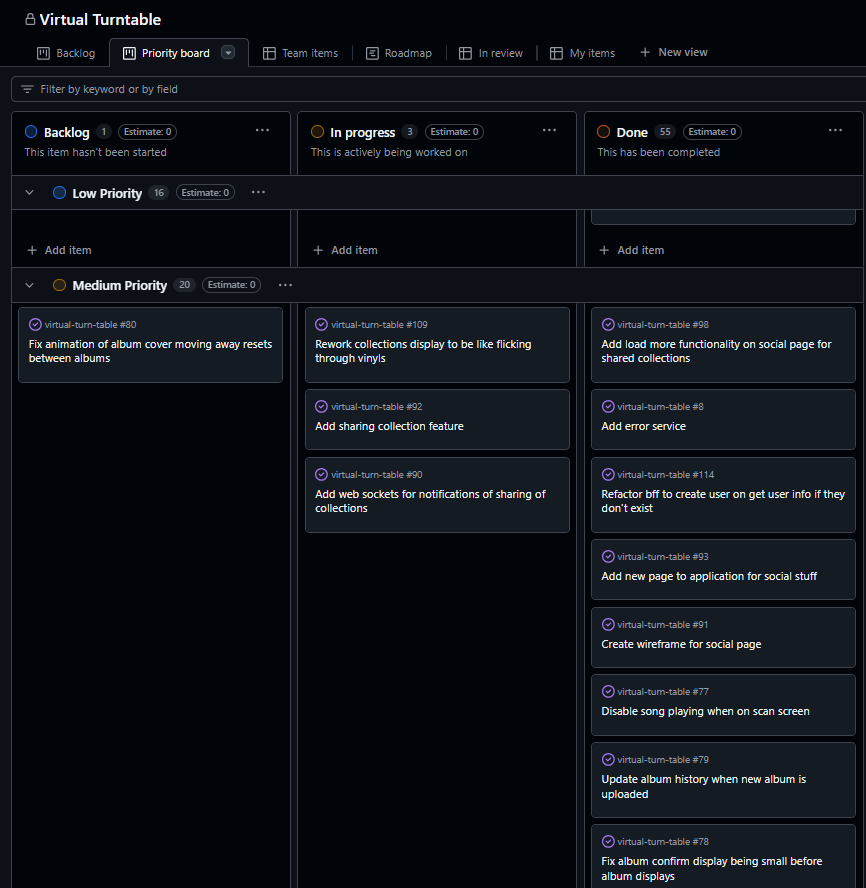
\includegraphics[width=0.65\linewidth]{figures/kanban_board.png}
    \captionsetup{justification=centering,margin=2cm}
    \caption{The Kanban board used during the project with tickets across the three columns}
    \label{fig:kanban-board}
\end{figure}

\subsection{Plan}
The plan for this project was structured into three key phases: design, development and testing, and deployment and maintenance.

\subsubsection{Design}
The first stage of the project involved finalizing the system design before commencing code development. This high-level planning approach addressed key architectural and technological decisions early in the process, ensuring a well-defined foundation. By making these decisions in advance, the need for ad hoc choices during development was minimized, reducing the risk of unintended consequences later in the project. This phase established the system's architecture, technology stack, deployment strategy, and user interface design, all of which are further detailed in Chapter~\ref{cha:design}.

\subsubsection{Development And Testing}
The development phase encompassed both the implementation of the core software and the integration of automated code quality tools to maintain consistency and reliability. A test-driven development (TDD) approach was adopted to ensure robust functionality. This included the creation of automated tests, reducing reliance on manual testing as the project scaled. Additionally, linters, formatters, and continuous testing were incorporated to enforce code quality standards as each commit was pushed to the repository, as further discussed in Section~\ref{sec:code-quality}.

The Kanban project planning system, outlined in Section~\ref{sec:plan-system}, played a crucial role in managing unforeseen challenges during development, such as bugs, which could be easily added to the board without disrupting the overall plan.

\subsubsection{Deployment And Maintenance}
Deployment was planned to involve hosting the system on a cloud platform to ensure accessibility for all potential users. The specific deployment method would be determined by the system’s design (Chapter~\ref{cha:design}), but a cloud-based solution was preferred due to its minimal cost for small projects and ease of configuration.

Maintenance was not a primary focus during planning; however, certain aspects were considered. Automated dependency management was planned, with bots monitoring the repository’s dependency files and updating them as new versions were released. Combined with the automated test suite, this approach ensured that dependencies could be updated with confidence and minimal manual intervention.

\chapter{Design}~\label{cha:design}
Before initiating detailed design work, it was decided this project would be a web application accessible via a browser. This approach offers several advantages, such as cross-platform compatibility, ease of access (requiring only a browser), scalability, and the ability to leverage existing web technologies~\cite{6822300}. With this established, a plan was formulated, encompassing architectural decisions, technology stack selection, and the definition of testing criteria.

\section{Architecture}
The system architecture defines the overall structure of the project and the communication between its components. For this project, two architectural approaches were considered: a monolithic architecture and a microservices-based architecture.

\subsection{Monolithic}
For this project, the monolithic approach offers several benefits. With all code centralised within a single framework, development is simplified, and debugging becomes more straightforward. Additionally, initial deployment is less complex since only one program needs to be managed once development is complete~\cite{9109514}.

However, the monolithic design has its drawbacks. As the system grows, maintaining a large, integrated codebase can become increasingly challenging; test suites may grow more complex and time-consuming to execute. During deployment, a single fault could potentially bring down the entire system, resulting in a complete loss of service. Similarly, even minor updates would require redeploying the entire monolith, increasing the risk of downtime. Moreover, this approach does not scale as effectively for web applications; as user demand increases, the need to redeploy the monolith frequently to manage higher request volumes becomes a significant concern~\cite{9109514}.

Although the scope of this project is small and so the drawbacks of a monolithic approach would have minimal impact, it was determined that the project should be designed to be fully scalable. With the potential for future growth in features and user base, the limitations inherent in a monolithic architecture would eventually become a hindrance in this scenario. Consequently, the monolithic approach was ruled out in favour of a more scalable architectural model.

\begin{figure} [H]
    \centering
    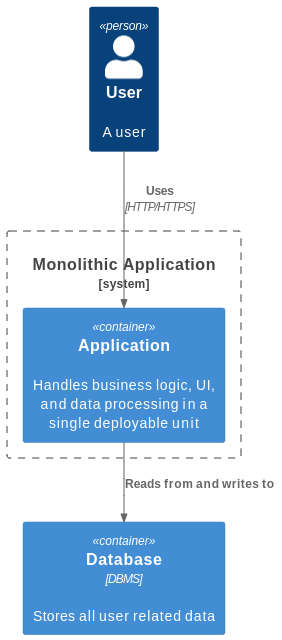
\includegraphics[width=0.35\linewidth]{figures/monolithic_arch.png}
    \caption{A potential architecture for a monolithic approach}
~\label{fig:monolith-arch}
\end{figure}

\subsection{Microservices}
The alternative approach examined was the use of microservices. In this architecture, the application's functionality is divided into separate services that communicate with each other using standardised protocols such as HTTP.\@

The primary benefits of this approach pertain to deployment and maintenance. Once deployed, the system can be scaled more efficiently—only those services experiencing high demand need to be replicated, which is significantly faster and more resource-efficient than scaling a monolithic system. Additionally, maintenance is simplified because each service operates independently; developers can focus on individual components without needing a comprehensive understanding of the entire system something that can become difficult even in small systems like this project.

However, the increased complexity of managing multiple services means that initial deployment is more challenging. Configuring the different addresses for inter-service communication can prove to be difficult, and each service requires setup that would only need to be completed once for a monolith. Nonetheless, once this initial configuration is completed, development within a microservices architecture becomes as straightforward as working with a monolithic architecture.

\begin{figure} [H]
    \centering
    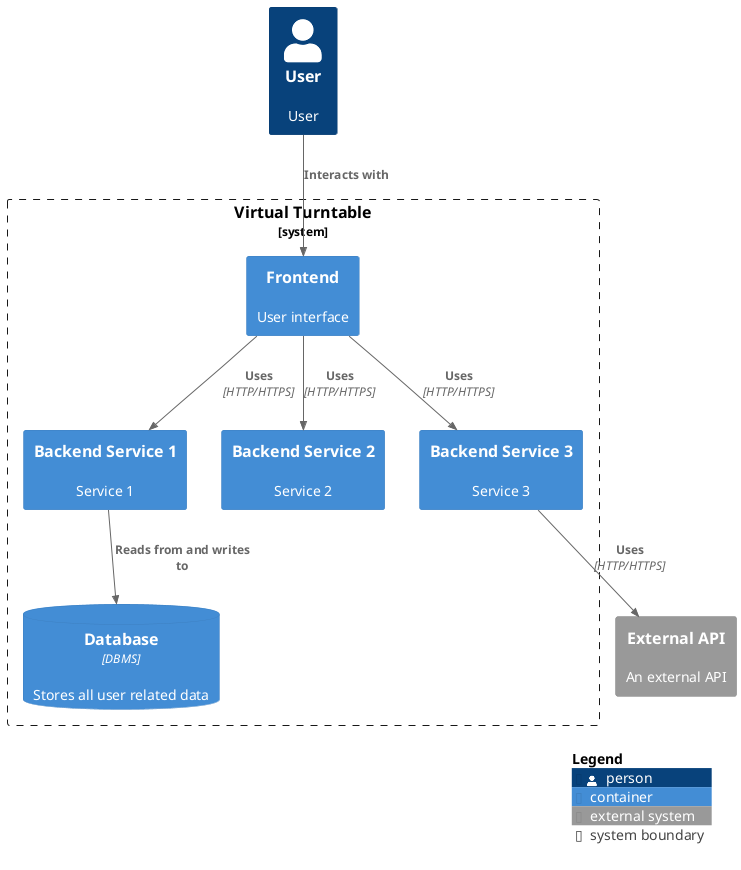
\includegraphics[width=0.5\linewidth]{figures/microservices_arch.png}
    \caption{A potential microservices design with three backend services}
    \label{fig:microservices-arch}
\end{figure}

\subsection{Final design}
The final design employs a microservices approach alongside a backend-for-frontend (BFF) design pattern. In this pattern, a dedicated backend service is created for each type of frontend application, such as desktop or mobile, ensuring that each backend caters specifically to a specific interface’s requirements. This pattern leverages the benefits of a microservices architecture and helps to maintain complexity by isolating functionality~\cite{BFF}. Details about each microservice are described in Section~\ref{sec:backend-design}.

\begin{figure} [H]
    \centering
    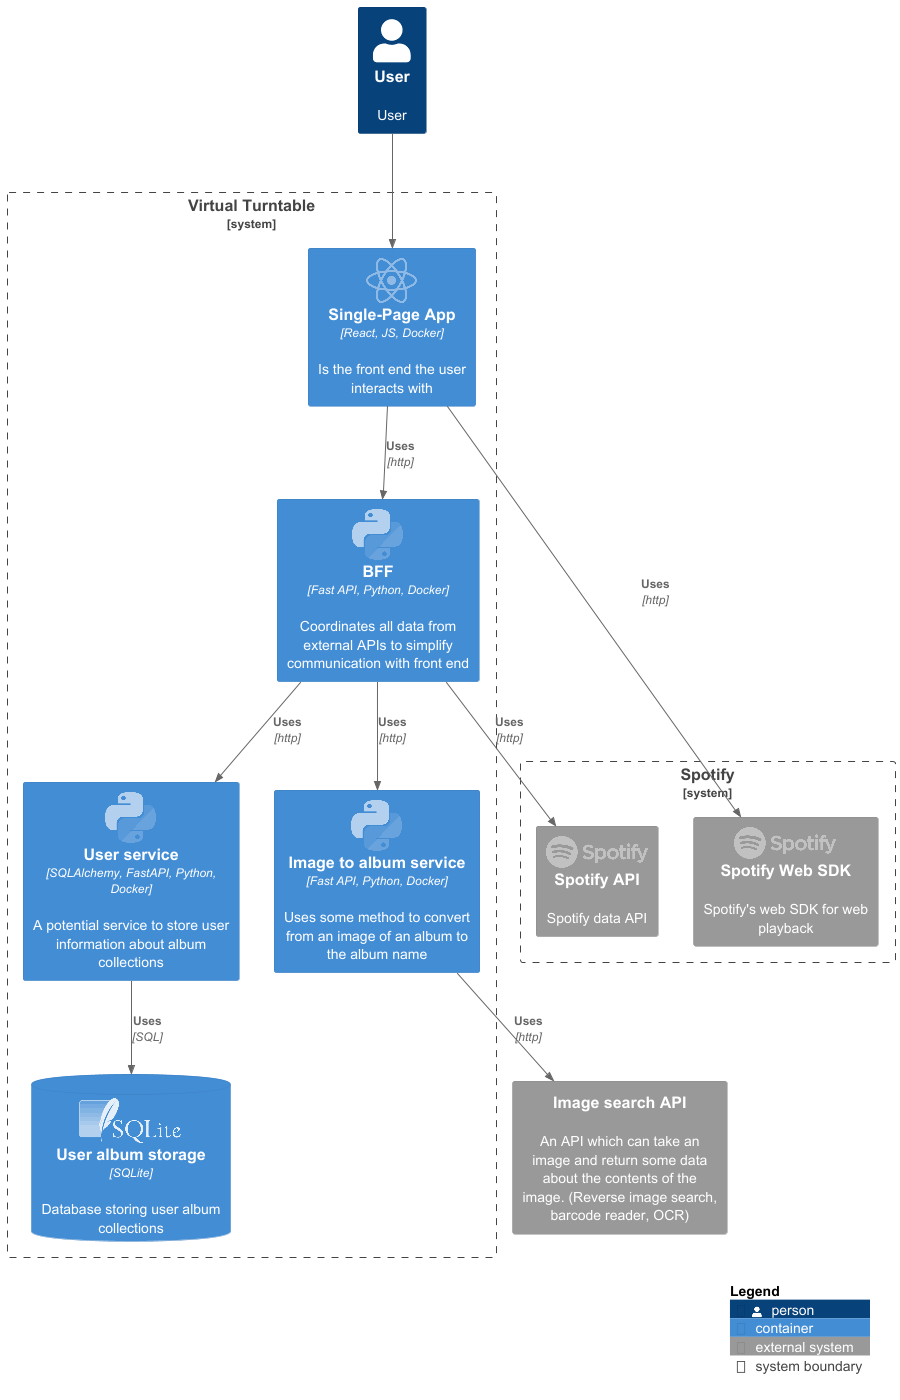
\includegraphics[width=0.5\linewidth]{figures/final_arch.png}
    \caption{The final architecture including technologies and external APIs}
    \label{fig:final-arch}
\end{figure}


\section{Technologies}
\subsection{FastAPI}
FastAPI is a Python web framework for building APIs, offering automatic input validation via Pydantic and seamless relational database integration with SQLAlchemy~\cite{FastAPI}. Compared to other popular frameworks like Django and Flask, FastAPI was particularly well-suited for this project due to its lightweight nature and built-in compatibility with these technologies. This combination provided an optimal balance between ease of setup and feature-rich functionality.

FastAPI was extensively utilised to develop all backend services in this project. Its straightforward setup allowed for rapid initial development, enabling quick implementation of basic functionality.

The backend primarily operated through individual API endpoints, which the frontend called to retrieve data as needed. Additionally, WebSockets facilitated asynchronous server-to-client communication, ensuring users were promptly notified of backend events, such as collections being shared with them.

\subsection{React}
React is a JavaScript library for building interactive web interfaces~\cite{React}. Its modular, component-based architecture was particularly beneficial in this project, enabling component reuse across multiple pages and reducing code duplication. A key advantage of this approach is the availability of extensive component libraries that provide pre-built functionality and styling for low-level elements, such as buttons. This allowed development efforts to focus on the application's bespoke features.

For this project, the HeroUI component library was utilised, offering a set of pre-designed components that were assembled into larger, more complex UI elements to create the final application.

React also managed the application's state and handled backend requests as needed. This enabled backend services to remain stateless, reducing complexity and improving scalability.

\subsection{Docker}
Docker is a platform for containerising applications, allowing them to run in isolated environments while communicating through specified exposed ports. This approach is a standard practice in modern web development and is widely supported by cloud providers, simplifying deployment and providing a consistent environment across different platforms.

For this project, Docker enabled fast and efficient deployment. Cloud providers could autonomously build and run the application when supplied with the codebase and Dockerfile. Additionally, for development, the containerised system could be easily executed on any device running Docker, eliminating the need for manual environment configuration.

All backend services and frontend, were containerised using Dockerfiles and deployed to a cloud provider, ensuring a scalable and reproducible deployment process.

\subsection{Spotify API And Web Playback}
The music service Spotify offers a suite of APIs for music-related services, including search and playback functionalities that matched the core features of this project. Given the impracticality of maintaining an independent album database, offloading the responsibility of maintaining a library of albums and music to Spotify was a logical choice.

Specifically, the search API was used to identify albums, while the playback API enabled streaming of the selected content.

However, a key limitation of this approach is that the playback API requires a Spotify Premium subscription. Though, as the Spotify API mandates user authentication via a Spotify account, this requirement allows the Spotify account to serve as the user account for the application, thereby reducing security concerns related to the storage and management of user data.

\subsection{Reverse Image Search}~\label{sec:reverse-image-search}
Reverse image search is a form of content-based image retrieval that uses an image as the query to retrieve related results. This process involves extracting feature vectors, using algorithms such as SIFT, and comparing these against a collection of previously indexed images to return the closest matches~\cite{Gaillard2017LargeSR}.

In this project, reverse image search functionality was implemented to identify albums from images uploaded by users. Recognizing that maintaining an up-to-date, in-house database of album covers would be impractical, it was decided early on to leverage an external API.\@ Two reverse image search APIs were evaluated: Google and Bing. Although Bing's API was simpler to integrate, it frequently failed to accurately identify albums—even from images that were already indexed by Bing's image search. In contrast, Google's API demonstrated a much higher reliability in album identification. Given the critical importance of accurate album retrieval for the project, the Google API was ultimately chosen.

Compared to other methods for recognizing albums from images, such as optical character recognition (OCR) or barcode scanning, reverse image search was selected for its robustness. OCR can be unreliable when album covers feature stylised text or lack text entirely and barcode scanning, though dependable, requires a barcode to be present. This requirement is problematic, particularly since vinyl records may predate the widespread use of barcodes.

\subsection{Google Cloud}
Google Cloud is a suite of cloud services offered on a pay-as-you-use basis. In this project, two specific services were utilised: the reverse image search API and Google Cloud Run. The reverse image search API was employed to identify albums from images uploaded by users, as detailed in Section~\ref{sec:reverse-image-search}. Google Cloud Run was used to build and host the application, running in Docker containers.

Although multiple cloud providers were available, Google Cloud was selected following the adoption of Google's reverse image search API.\@ For convenience, hosting the application on Google Cloud was simpler as it eliminated the need to manage services across different providers.

\section{Frontend}
The frontend is the user facing part of the application, because of this it needed to be designed with the knowledge that users have a wide range of abilities and needs. This meant that the user interface needed to be intuitive and easy to use.

A `multipage' design approach was selected for the application as this separates the application into sections, so the user is not overloaded on a single page. This could have been implemented in two ways, a router design where the separate pages are loaded as the user navigates the application or a single page app where the screens are different `tabs'. The former would have been simpler as there would be little to no implementation to link the pages together, but it was decided to implement later. This was done as it was thought this would provide a more fluid user experience where the user could easily switch between different views. This also had the benefit of allowing music playback to continue even as the user navigates the application.

\subsection{Principles}
An easy way to ensure that the user interface is well-designed is to follow a set of principles. A good example of these would be Shneiderman's eight golden rules of interface design~\cite{Shneiderman} which were used as a guideline in this project to ensure that the user interface was intuitive and easy to use. %These rules are as follows:
\iffalse
\begin{itemize}
    \item Strive for consistency
    \begin{description}
        \item[] The design should be consistent throughout the application, components should look and behave the same way wherever they are used.
    \end{description}
    \item Seek universal usability
    \begin{description}
        \item[] Users have diverse needs and abilities, so the design should not exclude any potential users.
    \end{description}
    \item Offer informative feedback
    \begin{description}
        \item[] There should be feedback to user actions, such as dialogue boxes, loading spinners, or page transitions.
    \end{description}
    \item Design dialogues to yield closure
    \begin{description}
        \item[] Actions in the application should have some sort of logical structure
    \end{description}
    \item Prevent errors
    \begin{description}
        \item[] Users should not be allowed to do things that would cause errors, for example buttons should be disabled if they should not be used.
    \end{description}
    \item Permit easy reversal of actions
    \begin{description}
        \item[] Users should be able to undo actions, for example, a confirmation dialogue before deleting something.
    \end{description}
    \item Keep users in control
    \begin{description}
        \item[] Users should feel the application is acting as they intend it to, there should be few surprises, and behaviour should be predictable.
    \end{description}
    \item Reduce short-term memory load
    \begin{description}
        \item[] There should only be a small amount of information of the screen at one time, and the user should not have to remember things from one screen to another.
    \end{description}
\end{itemize}
\fi

\subsection{Wireframe mockups}
Prototyping the user interface provides a rapid way to visualize the application, enabling design evaluations without the need to write any code. This approach proves especially beneficial during the early stages of development, when the design remains flexible and can be easily modified. In this project, wireframe mockups were selected for their low-fidelity nature, which allowed fast iteration on design.

Across all mockups, a consistent navigation bar is present at the top of the screen, allowing for straightforward navigation among the application's various pages.

\subsubsection{Play Screen}
Figure~\ref{fig:play_screen_mockup} depicts the mockup of the play screen, where users control music playback. Essential functionality implemented here includes buttons to play, pause, skip forward or backward, adjust the track position, and manage volume. Fitting with a modern streaming service, individual tracks can be played from the album, even though this would not be commonly done with a physical turn table.

The screen is also designed to incorporate elements of a physical turntable as part of the theme. Mainly the spinning vinyl seen in the centre.
\begin{figure} [H]
    \centering
    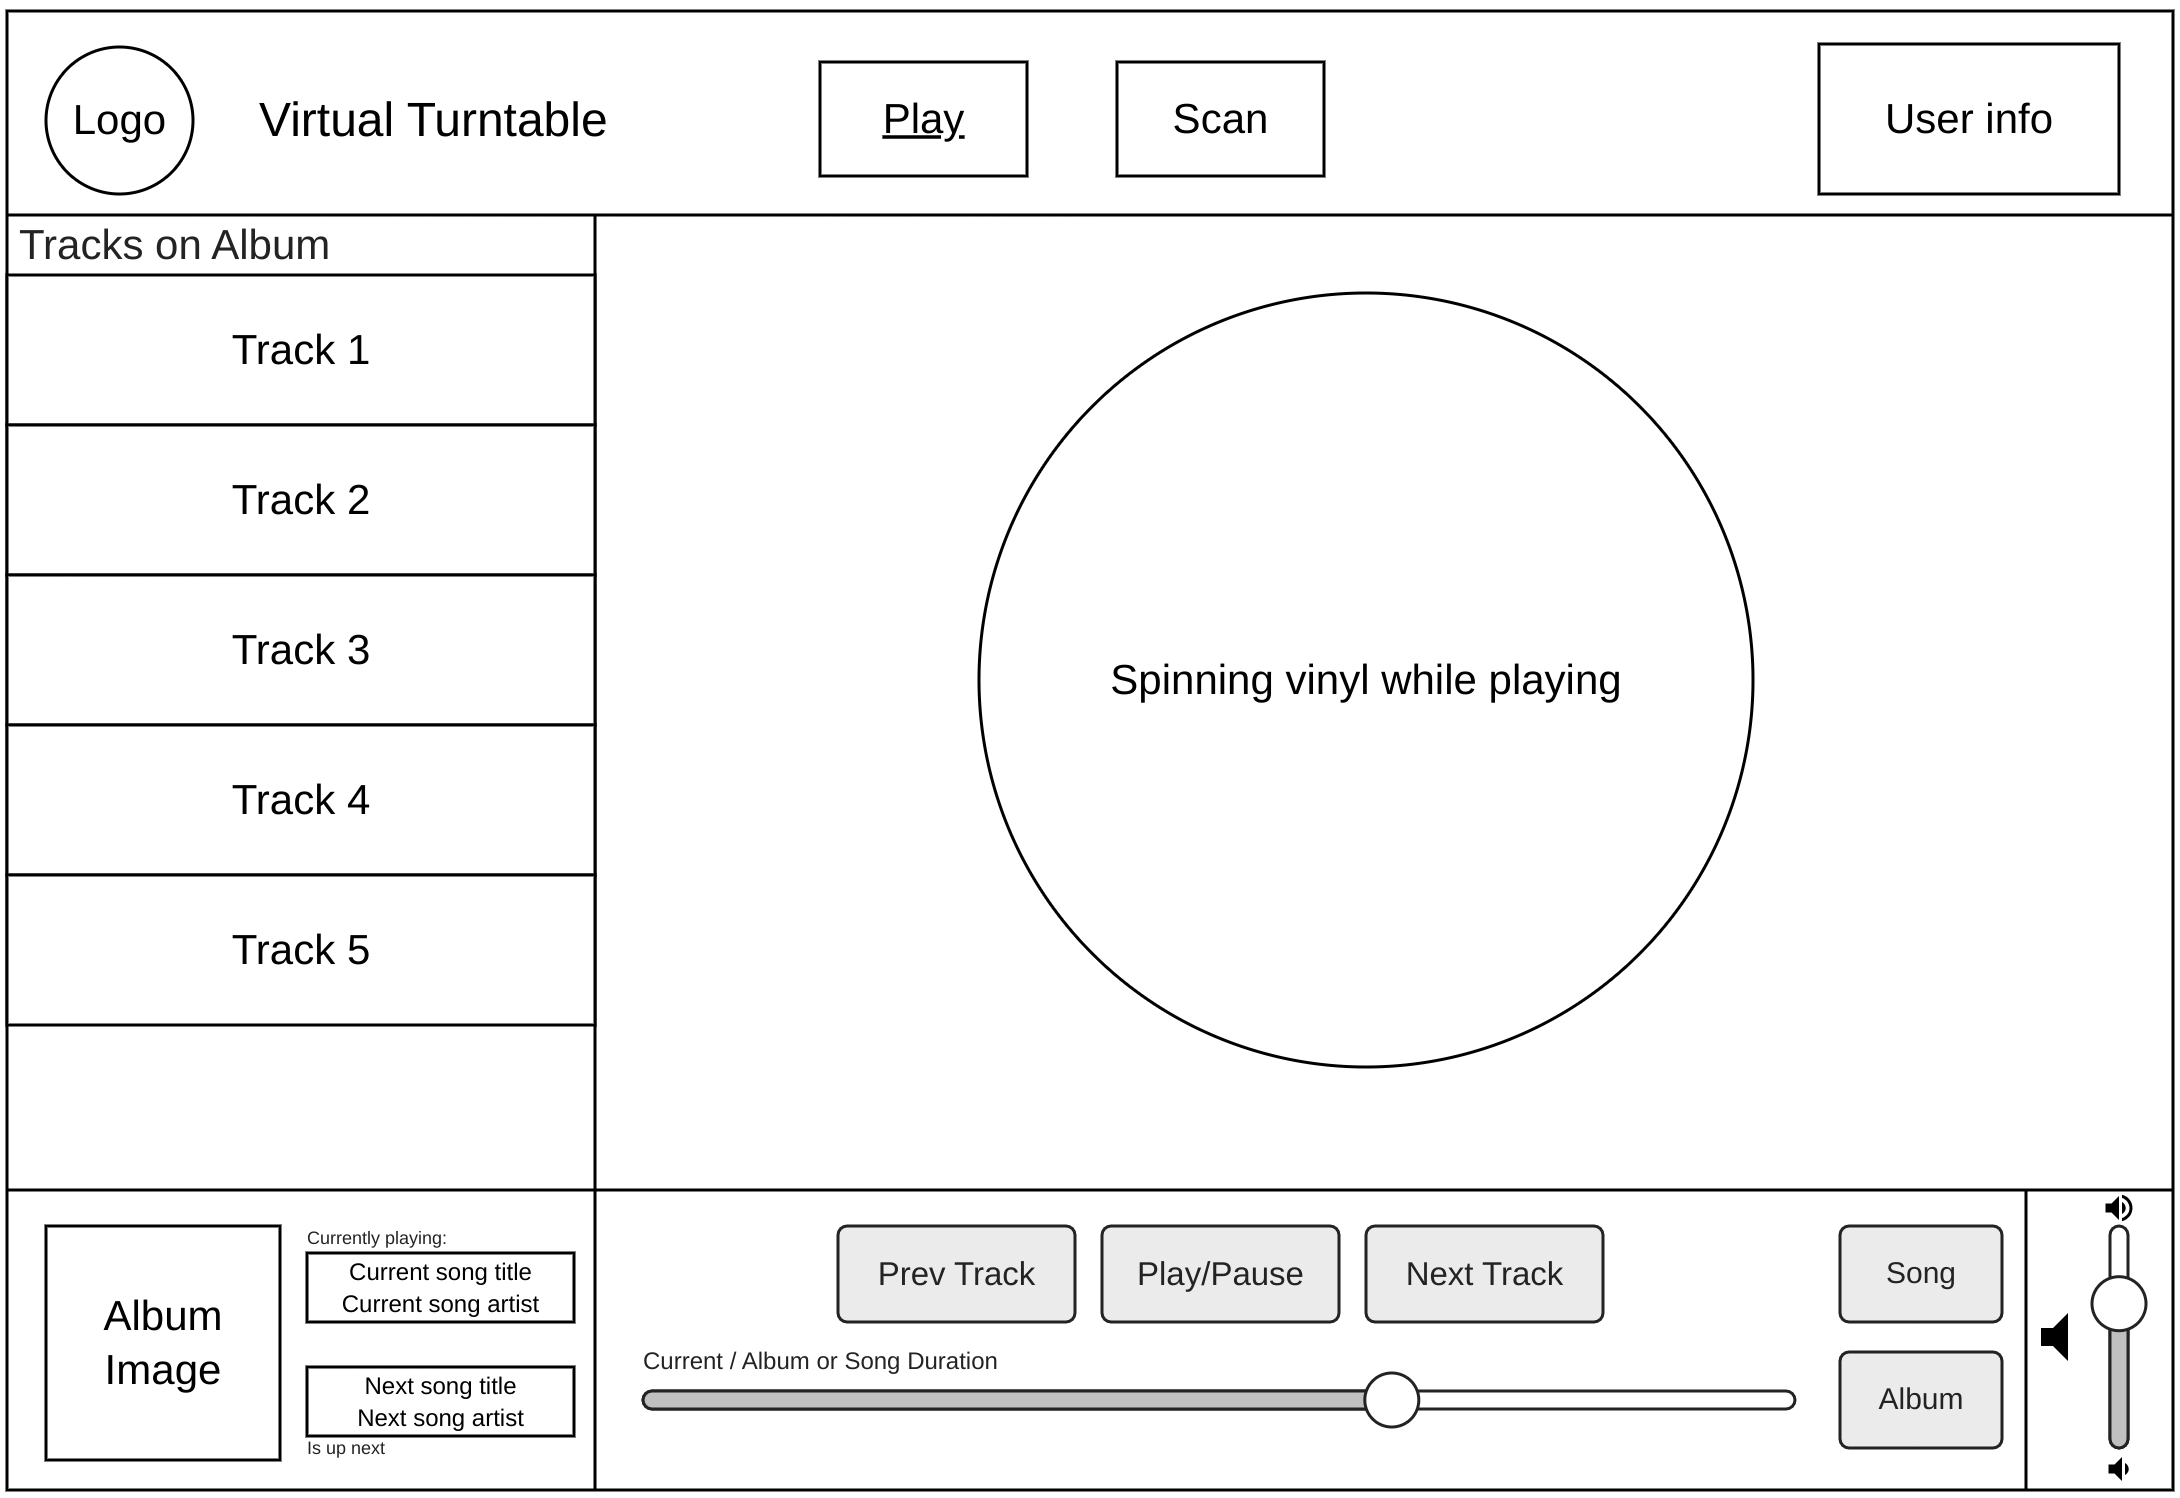
\includegraphics[width=0.6\linewidth]{figures/play_screen_mockup.png}
    \caption{The play screen wireframe mockup}
    \label{fig:play_screen_mockup}
\end{figure}

\subsubsection{Scanning Screen}
Figure~\ref{fig:scan_screen_mockup} shows the scanning screen, where users can upload images of album covers to identify the corresponding album. It also displays the logged-in user’s existing album collection, allowing quick selection of albums already scanned. The confirmation dialogue (shown on the left) enables users to confirm the identified album or reject it if incorrect.

\begin{figure} [H]
    \centering
    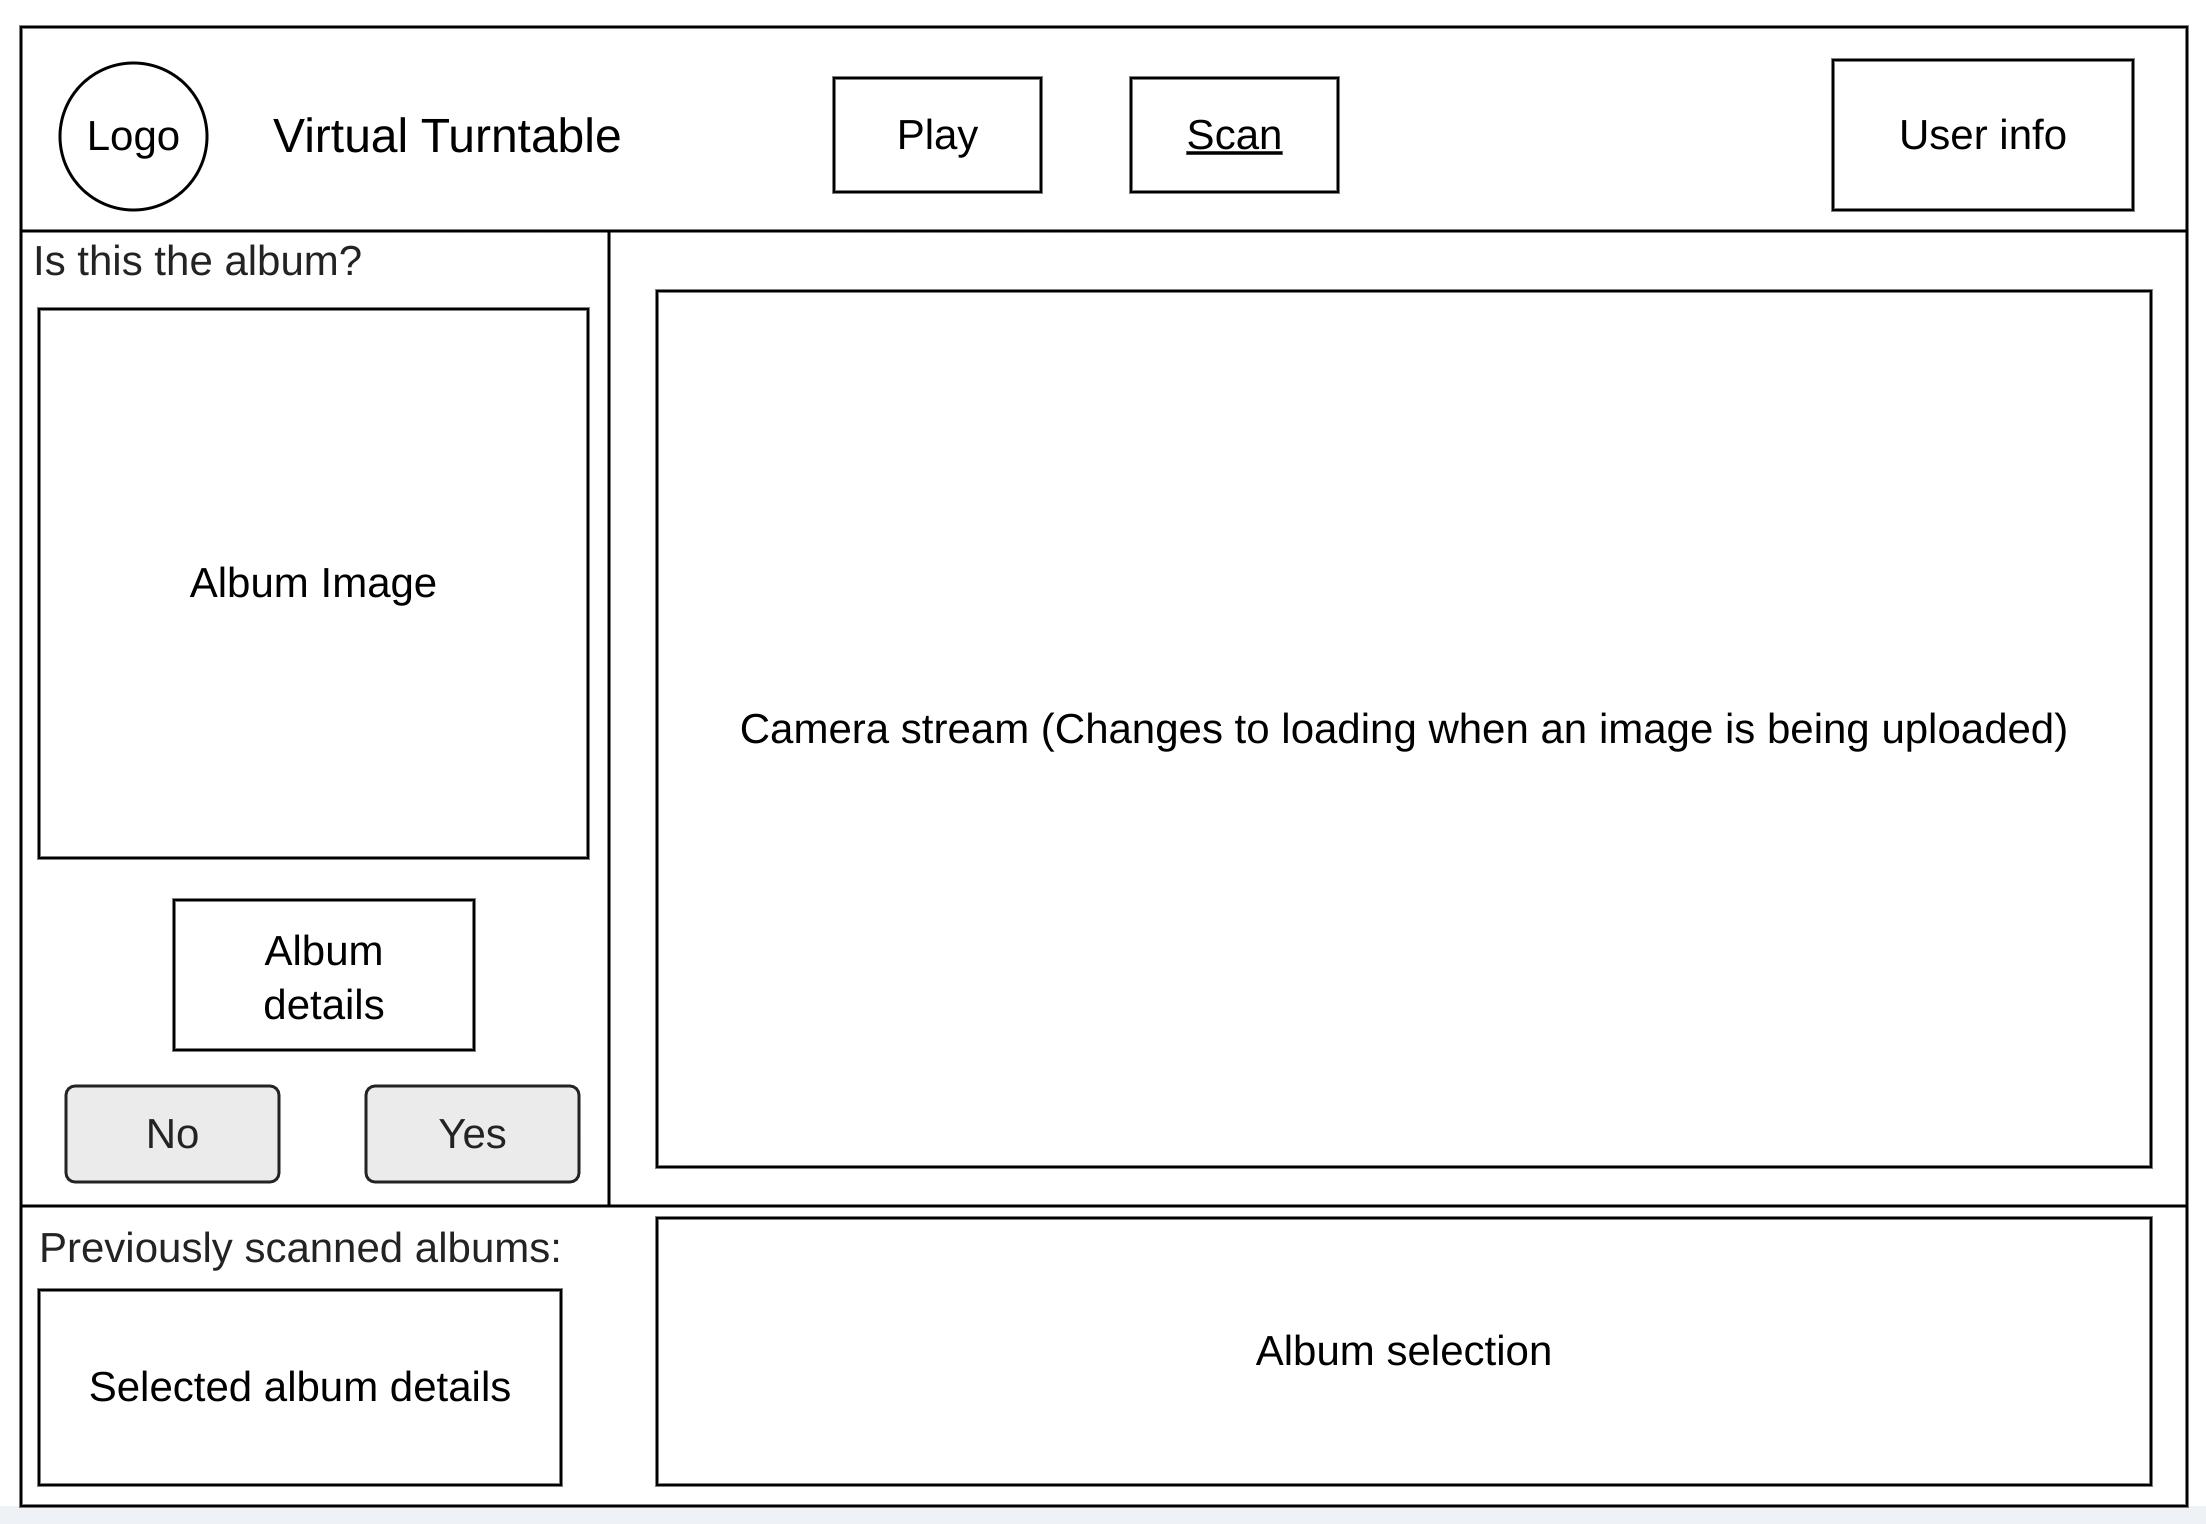
\includegraphics[width=0.6\linewidth]{figures/scan_screen_mockup.png}
    \caption{The scanning screen wireframe mockup}
    \label{fig:scan_screen_mockup}
\end{figure}


\subsubsection{Social Screen}
Figure~\ref{fig:social_screen_mockup} shows the social screen, where users can view collections belonging to others shared directly with them or made public by other users. This feature aimed to add a sense of social interaction among users and allow for the discovery of new music.

%Initially, albums were displayed in columns, but this layout proved limiting for users with extensive collections as it required excessive scrolling. Moreover, this featured presented an opportunity to capture the feel of browsing through a physical record store, prompting a revision of the layout to accommodate larger collections more intuitively. TODO: ref later section about development

\begin{figure} [H]
    \centering
    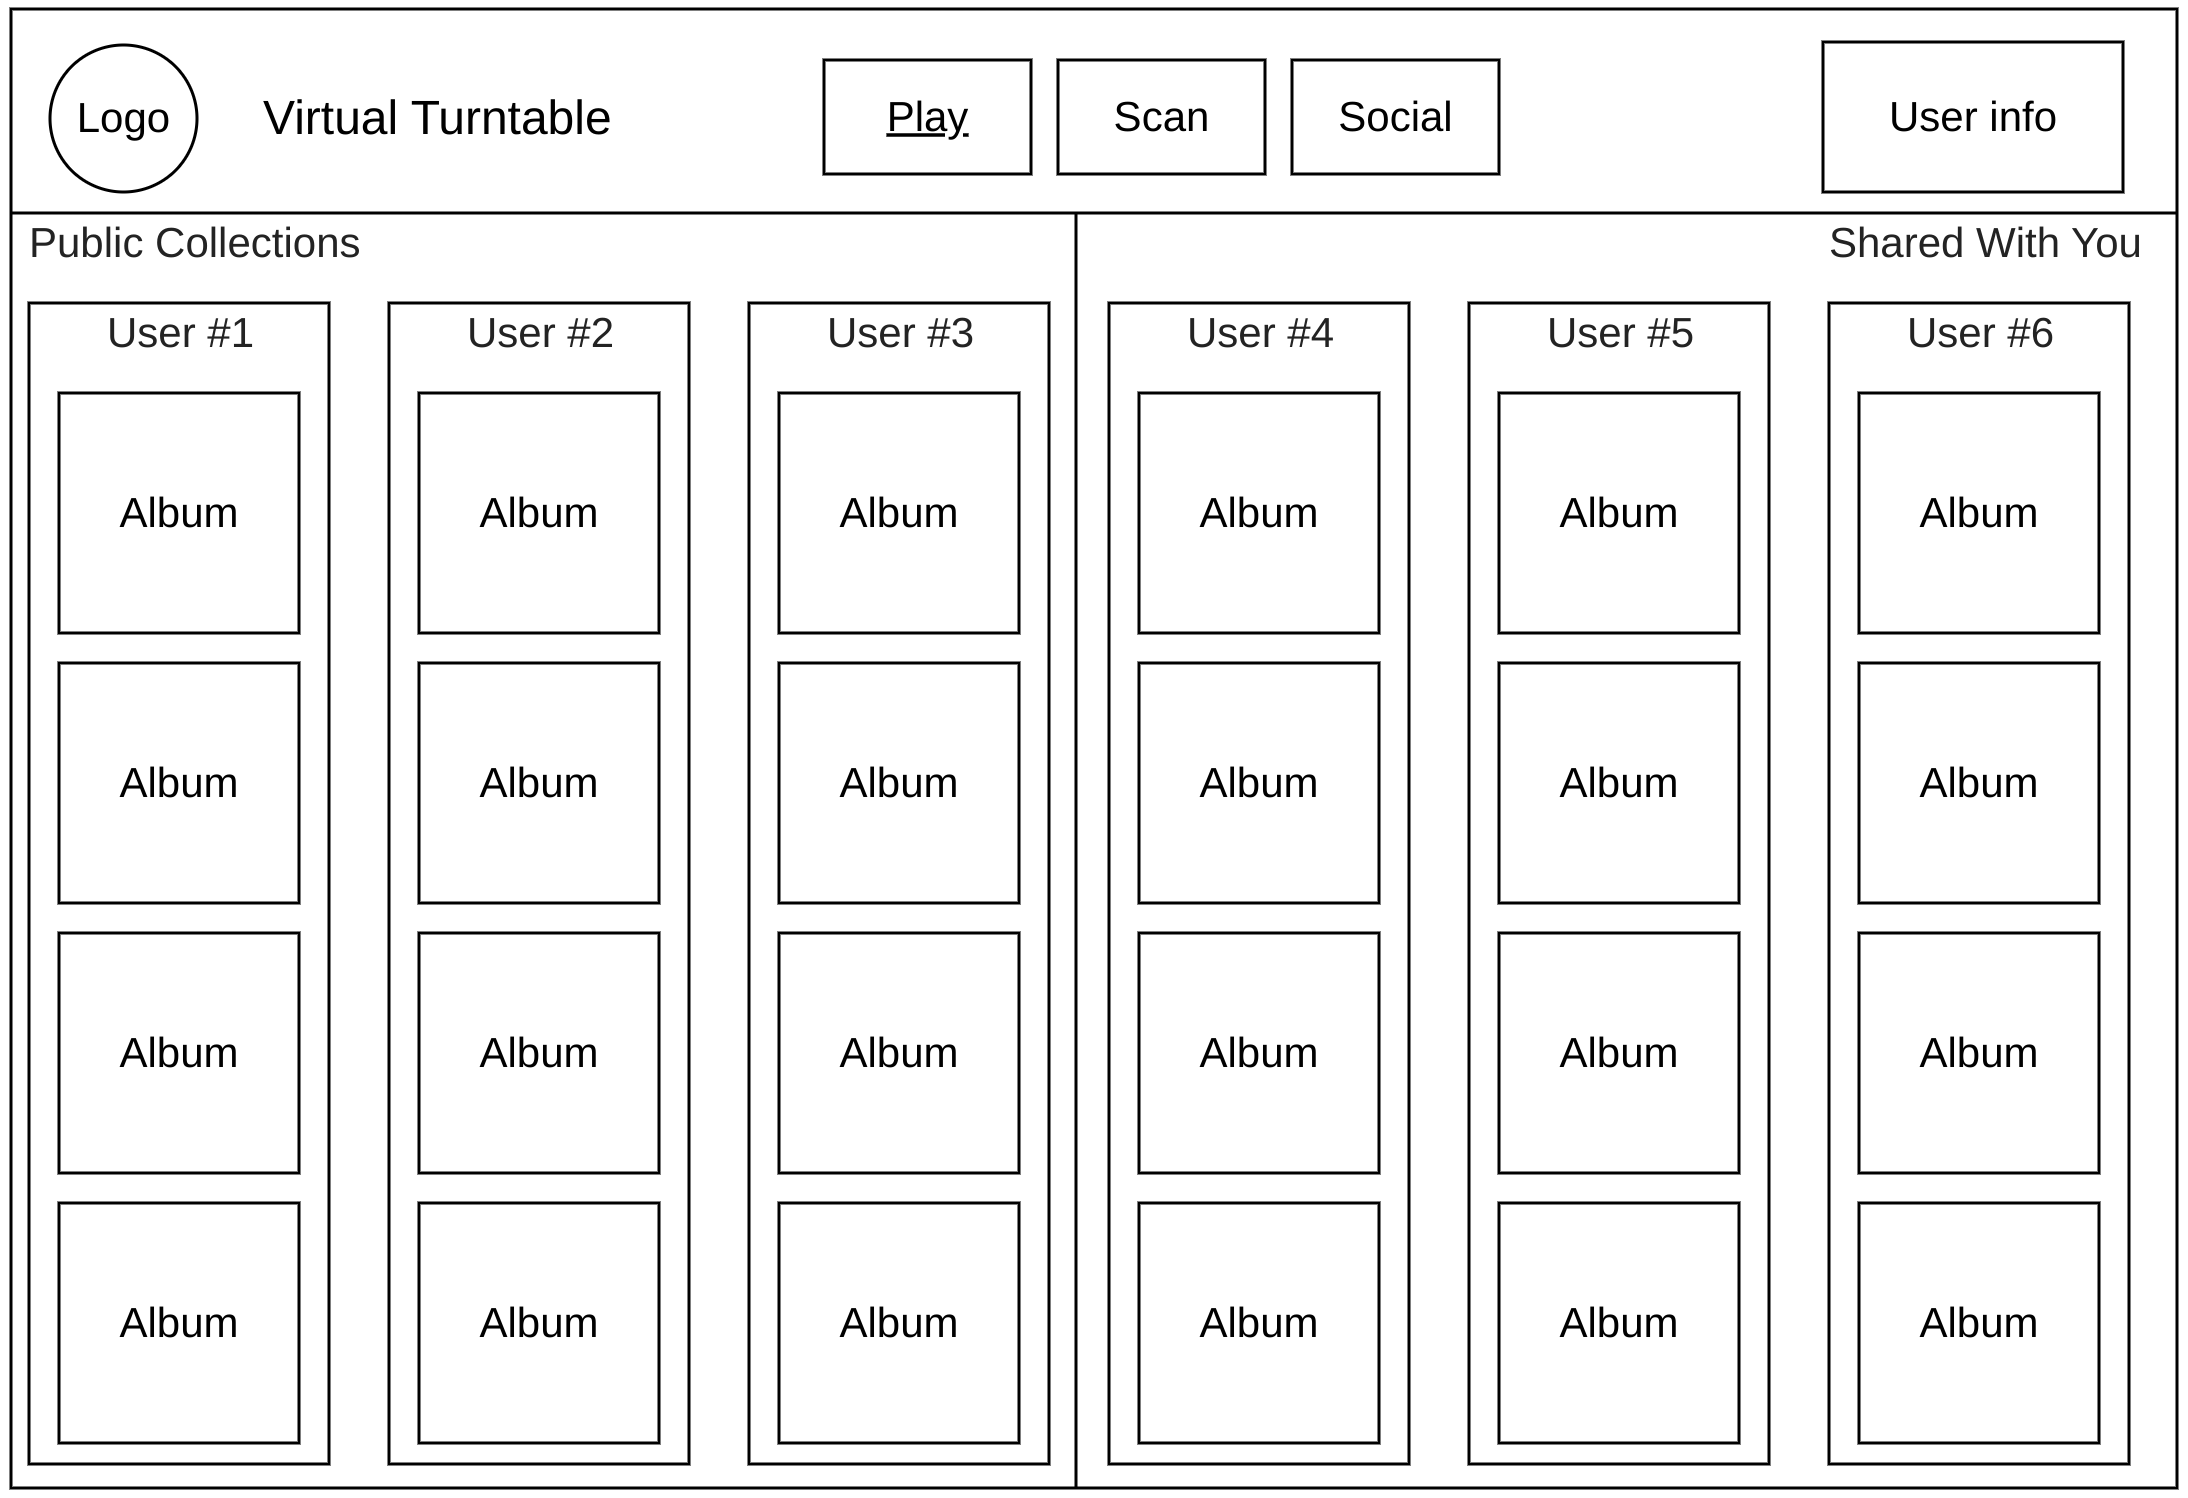
\includegraphics[width=0.6\linewidth]{figures/social_screen_mockup.png}
    \caption{The social screen wireframe mockup}
    \label{fig:social_screen_mockup}
\end{figure}

\section{Backend}~\label{sec:backend-design}
The backend for the project would responsible for handling all business logic and data handling. It would mostly respond to API calls from the frontend except in cases where the backend would need to asynchronously push data to the frontend. This would be done using WebSockets.

\subsection{Microservices split}
As a microservices approach was adopted, the backend operations were divided into multiple services. As described in Section~\ref{fig:final-arch}, it was decided to use a BFF (Backend for Frontend) pattern for one of these services. The remaining functionality was split into two services; one service handles the conversion of user-uploaded images into album data, while another manages all user-related data storage.

\subsubsection{BFF}
The BFF acts as a middleman between the frontend and various backend services, often mirroring the endpoints of those services. Its main responsibility is to manage the data returned to the frontend. As this project is focused solely on a desktop web application, so the patterns potential to tailor data for different platforms was not fully utilised. However, if the application were later expanded to include additional platforms, the BFF could selectively limit data returned to given devices if they did not require it.

The BFF also handles the WebSocket connections to the frontend, allowing the backend to push data to the frontend when necessary. This is particularly useful for notifying users of new shared collections or other events that require immediate attention.

\subsubsection{Image to Album}
This service was the smallest of the three, encapsulating a very specific functionality. It included endpoints responsible for identifying albums from various inputs, such as images of the album, allowing different methods, such as OCR or reverse image search to be handled through separate endpoints with the caller choosing which to use. Along with that the service also hosted a way to search for albums using Spotify's API as a method to return an exact album from a guess that might have been generated by an identification method.

Separating these functions from the rest of the application’s services means users could still listen to their existing collections in the event that this service going down.

\subsubsection{User Data}
This service was to handle all tasks related to user data such as collections and sharing. It would do this by interacting with a database detailed in Section~\ref{sec:database}. Each endpoint would be responsible for editing the data in the database in some way such as creating a user or sharing a collection.

\subsection{Database}~\label{sec:database}
This application could have been implemented as a stateless application which would  mean there was no capability to persist data across sessions. However, such an approach would limit functionality as there could be no form of personalisation for individual users. Since a Spotify account was already required for music playback, linking user data to that account became a logical next step, enabling data persistence across sessions.

\subsubsection{SQL vs NoSQL}
SQL databases are widely used in enterprise environments due to their reliability and consistency. However, they are not necessarily optimal for web applications requiring high scalability and availability~\cite{GANESHCHANDRA201513}. In contrast, NoSQL databases are designed with scalability and availability in mind~\cite{NoSQL}, often making them more suitable for such applications.
Although a NoSQL database like MongoDB would have been a good choice for this project, a SQL database was selected for its easy integration with FastAPI and SQLAlchemy. This meant quicker development and cleaner code, despite not being the most inherently scalable option.

\subsubsection{Diagram}
\begin{figure} [H]
    \centering
    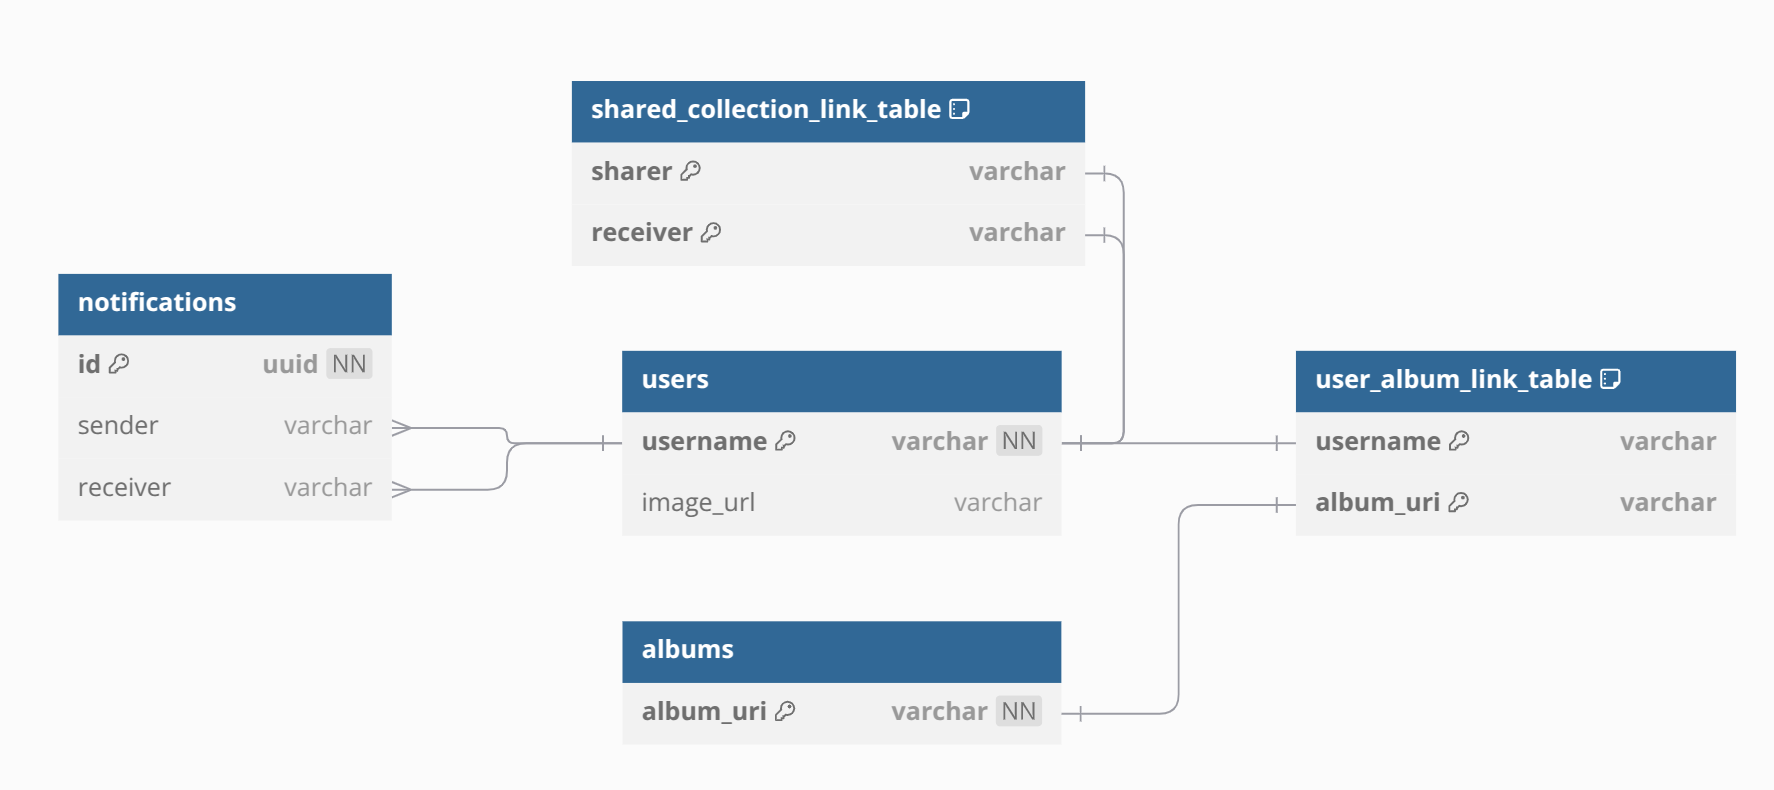
\includegraphics[width=0.6\linewidth]{figures/db_diagram.png}
    \caption{A diagram of the database using crow's foot notation}
    \label{fig:database-diagram}
\end{figure}

Figure~\ref{fig:database-diagram} shows the database design. User are stored with their Spotify usernames as primary keys as Spotify guarantees unique usernames. This allows data in other tables to be linked through each user’s username. Collections are represented with a link table that captures the many-to-many relationship between users and albums. A similar link table structure is used to manage the sharing of collections, tracking which users have shared access with each user. In addition, notifications regarding newly shared collections are stored in a separate table, so they can be displayed to users upon login.

\subsubsection{DBMS Choice}
Since the choice was made to use a relational database, a specific relational database management system had to be selected even though the use of SQLAlchemy abstracts many of the differences among various DBMSs allowing one system to be swapped out for another with no code changes. The only notable exception is that SQLite does not enforce foreign key constraints by default, requiring manual enablement.

Originally, SQLite was chosen because, as since it's a file-based database, it could be easily stored within the Docker container running the user data service, which would simplify deployment by reducing the number of containers. However, as the project grew, the need for concurrent database access became apparent which SQLite does not support. Because of this the decision was made to switch to either MySQL or PostgreSQL, both of which support concurrent access. For the purposes of this project, the differences between these two systems were minor. PostgreSQL was selected since it is open-source, which reduces the risk of support being dropped in the future.

\subsection{Security}
Security is an important consideration for any web application, since functionality and access to user data is exposed to the internet. Although the stored user data in this project is not particularly sensitive, it should still be safeguarded. To ensure this measures had to be implemented for each backend service.

\paragraph{BFF} The BFF represents the largest potential security risk, as it is the only service that directly interacted with the frontend and therefore exposed to the public internet. To mitigate this risk, the BFF uses authentication to verify requests to all endpoints related to user data. This was handled via the API token provided by Spotify during user login, this meant access to user-specific data remained only accessible by that specific user.

\paragraph{Image-to-Album \& User Data Services} These services operate behind the BFF and only need to accept requests from that single, predictable source. Because of this, these services are designed to reject any requests originating from any external sources ensuring that only valid requests are processed.

\section{Testing}~\label{sec:test-design}
Defining the tests and success criteria prior to development was important to ensure that the project was built to meet these objectives, rather than retrofitting tests to match the final product. For most of the criteria listed in Section~\ref{sec:objectives}, it was necessary to establish tangible measurements to determine whether they had been met. This requirement led to the definition of the following tests for the primary features:
\begin{itemize}
    \item The application should correctly identify albums with at least 95\% accuracy.
    \begin{description}
        \item[Verification:] Take a set of input images, modified to be of both poor and good quality, and calculate the accuracy of the system. It is important that as the application will likely rely on external APIs for this functionality the accuracies of any APIs are taken into account.
    \end{description}
    \item The application should play an album from start to finish without interruption.
    \begin{description}
        \item[Verification:] Play a set of albums on the application and verify that they play without interruption.
    \end{description}
\end{itemize}

For the criteria relating to the user interface it becomes more difficult to define tests as they are more subjective. However, user feedback can be collected after users use the application in the form of surveys to gather opinions on the interface.

The last set of criteria, relating to good software development practices, are generally more objective and as such are more easily verifiable. For this the following tests were defined:
\begin{itemize}
    \item The codebase should maintain at least 95\% test coverage.
    \begin{description}
        \item[Verification:] Run all test suites and verify the line coverage and branch coverage exceed 95\%.
    \end{description}
    \item All tests must pass successfully.
    \begin{description}
        \item[Verification:] Run all test suites and verify that all tests pass.
    \end{description}
    \item Code should be evaluated by linters and formatters to maintain consistency and quality.
    \begin{description}
        \item[Verification:] For Python code, run ruff for formatting and Pylint for linting. For typescript run Biome for both formatting and linting. Both should pass without errors.
    \end{description}
    \item A continuous deployment system should automatically redeploy the application following any code change.
    \begin{description}
        \item[Verification:] Push a change to the repository and verify that the application is redeployed with the change in place.
    \end{description}
    \item An automated system should be in place to update dependencies.
    \begin{description}
        \item[Verification:] An automated tool for dependency management should be configured on the repository to run at a given interval.
    \end{description}
\end{itemize}

Most of these criteria can be met using tools such as GitHub Actions, which can run tests on each commit, and trigger application deployments. Dependabot can be used to scan the repository’s dependencies and update them as new releases become available. Additionally, linters and formatters can be executed as pre-commit hooks, preventing code below a defined quality threshold from being committed to the repository.

A side effect of having high test coverage is that there is a reduced risk associated with dependency updates, since tests help verify that no functionality has been broken by the update.

\chapter{Development}~\label{cha:development}
Development of the application was divided into two main parts: the frontend and the backend, with the backend further broken up into its constituent services. The entire project was maintained in a single mono-repository, with each backend service and the frontend housed in separate directories. While this is not necessarily the optimal structure for a larger project this approach reduced overhead for a project of smaller scope, making it the most practical solution.

\section{Frontend}~\label{sec:frontend-development}
\subsection{Implementation}
The actual implementation of the frontend used Vite as a development server and build tool for the React frontend. This gave a starting TypeScript template which was modified to create the application.

Once the build system was in place the design was broken up so that each component could be built independently. The HeroUI component library used in this project provided basic components common to most web applications, such as buttons, modals, and input fields from these the more complex components could be built. One of the benefits of using this component library was its integration with Tailwind CSS, which allowed for stylings to be applied through class names rather than bespoke stylesheets. This greatly reduced the amount of time needed to style the application and ensured a consistent look across the application.

After completing the frontend components, the next step was to integrate them with the backend services. Some functionalities required user authentication through Spotify to access key Spotify API features. This had to be implemented on the frontend using Spotify’s OAuth2 flow, which redirects the user to Spotify for login and then returns them to the application with an access token in the URL which is read by the application and saved to local storage, so sessions persist between refreshes.

Once the authentication was implemented, the remaining backend API endpoints were integrated using the Axios library, allowing the frontend to communicate efficiently with the various services.

Once the authentication was implemented, all remaining endpoint calls were implemented as functions that can be imported and run by any component. This was done using the Axios library, which though not a native JavaScript library, is widely used and well documented which made it easy to implement.

\subsubsection{Landing Page}
An oversight in the original design was the lack of a landing page which is presented to users before logging. The page follows the stylings of the application and contains graphics and text related to the application. Once the user logs the page is redirected to the scan screen. A landing page also gives the chance to give a brief overview of the application and its features as well as add visually appealing graphics which might improve the user's impression of the application.

\begin{figure} [H]
    \centering
    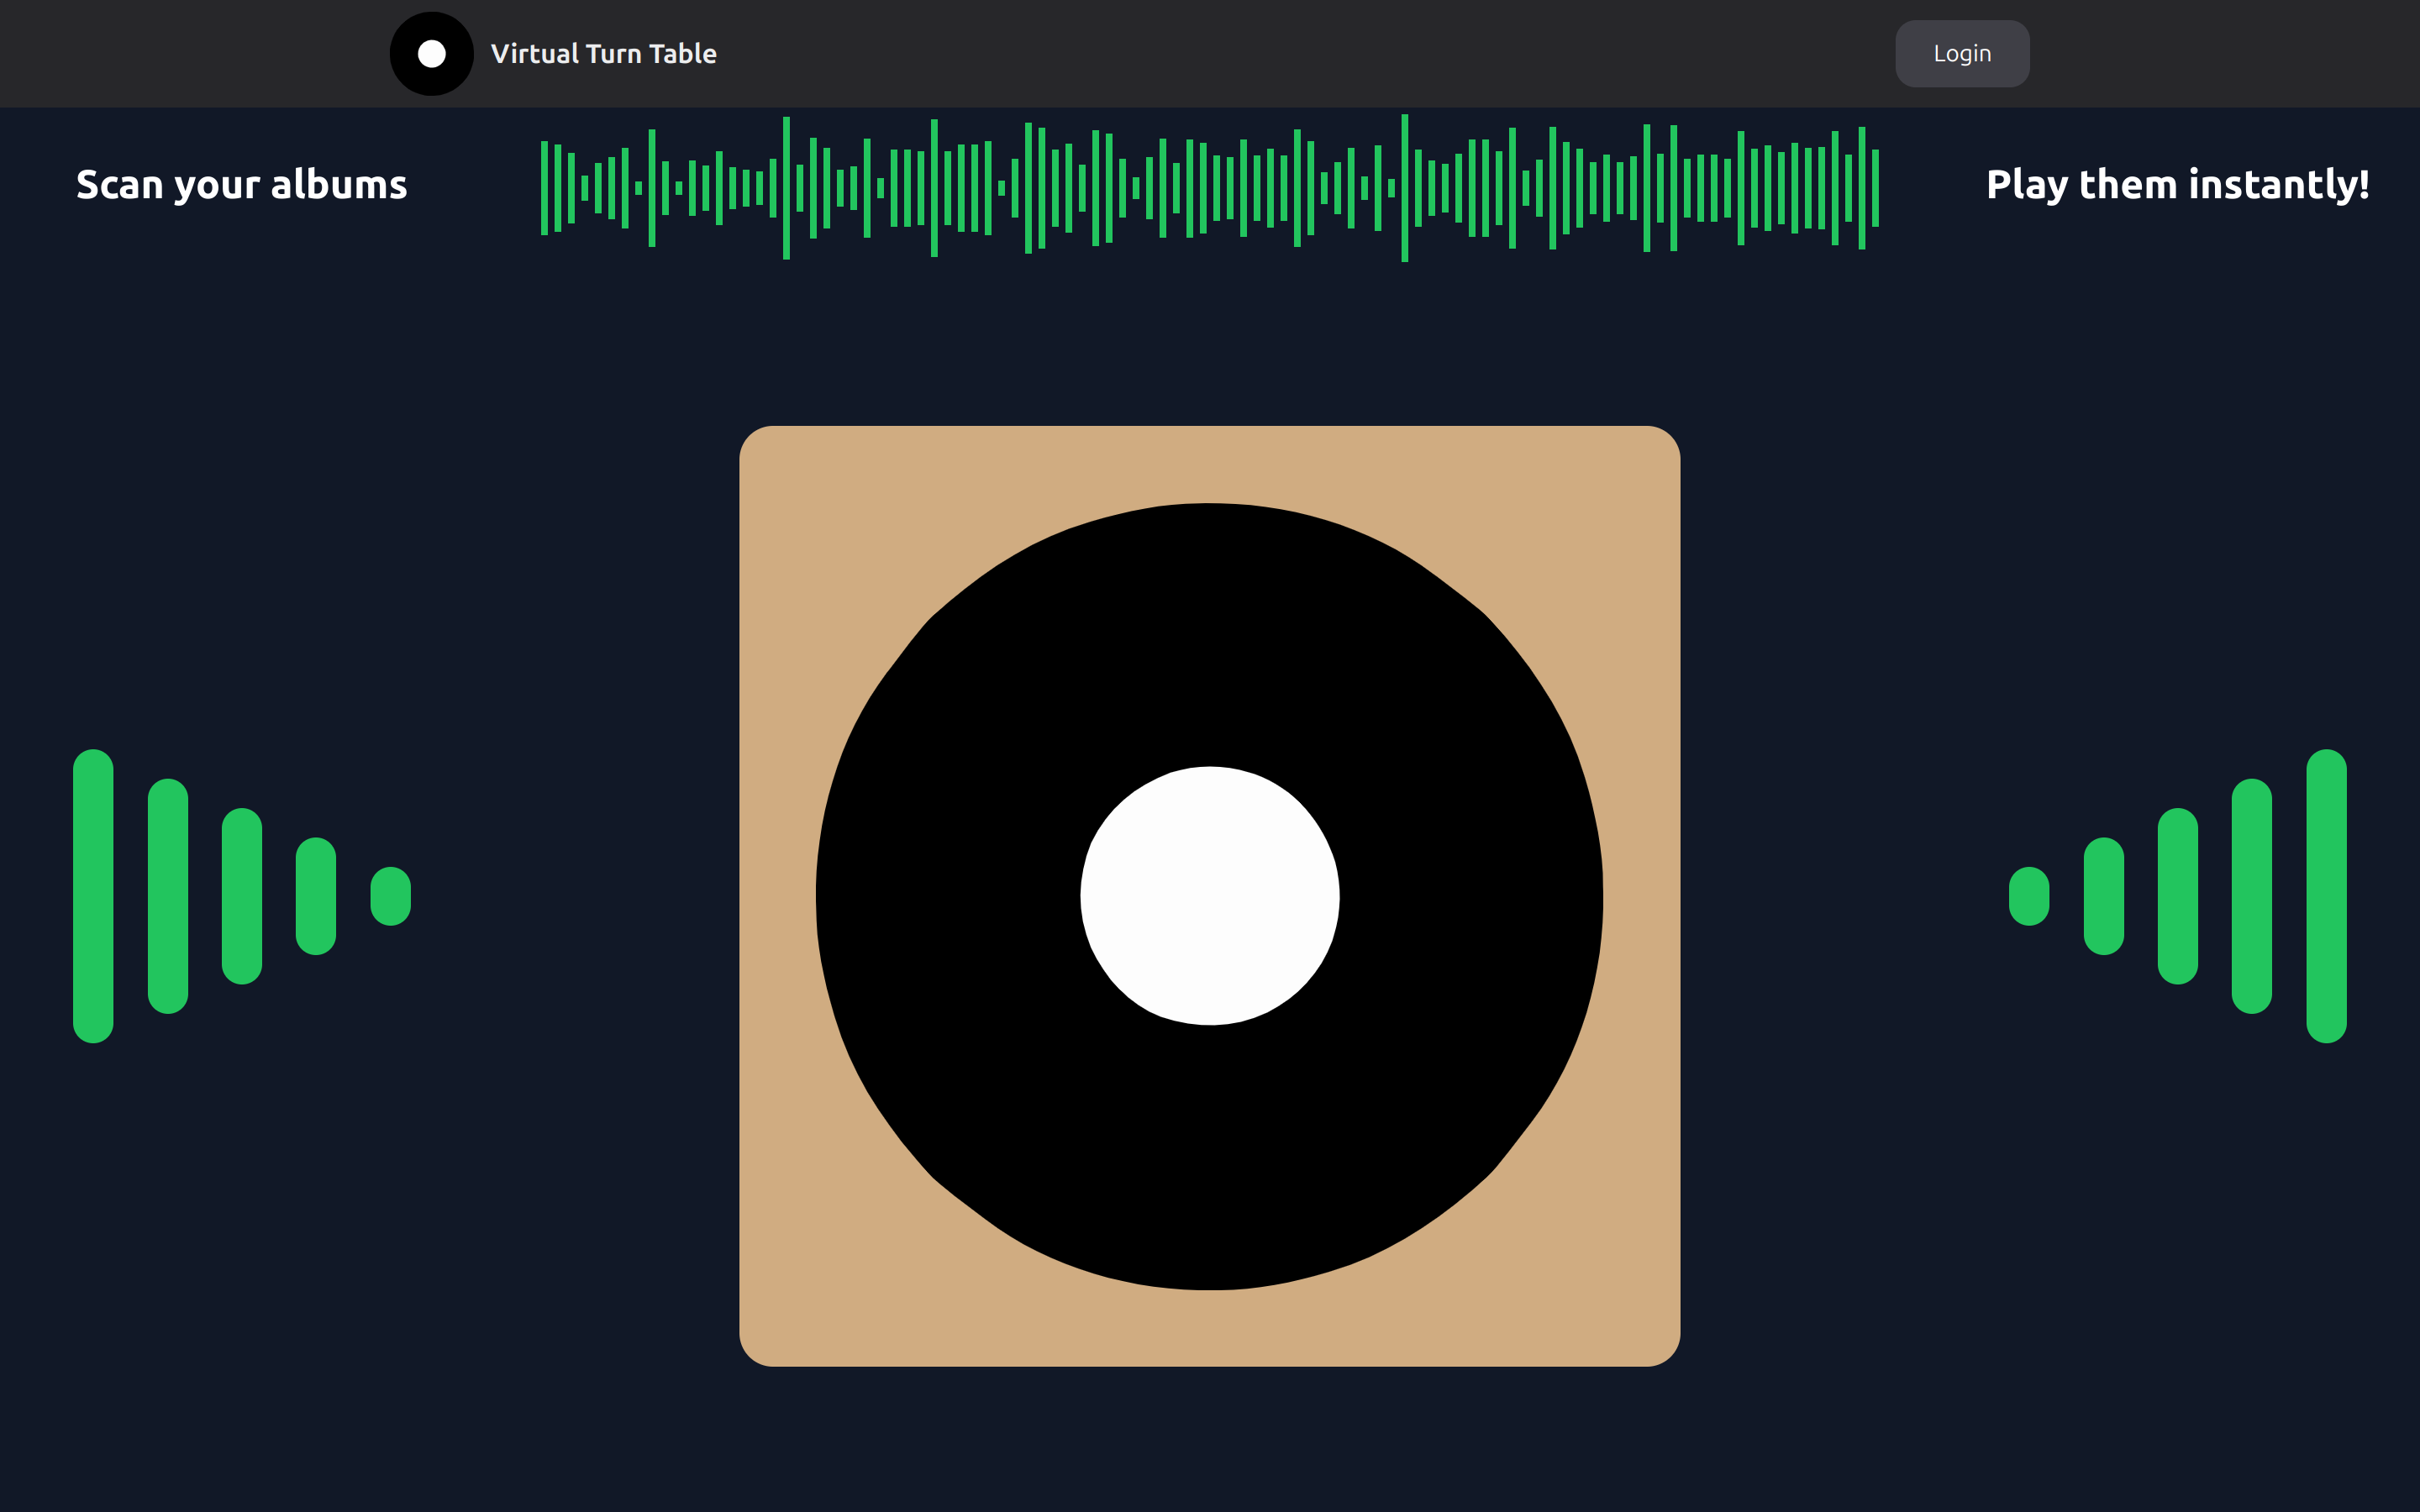
\includegraphics[width=0.8\textwidth]{figures/landing_page.png}
    \caption{The landing page of the application}
    \label{fig:landing_page}
\end{figure}

\subsubsection{Navigation Bar}
The navigation bar is a component included on all screens which allows the user to navigate between the different screens of the application. It consists of a static logo, screen selection tabs, and user details. The user details also serves as a dropdown trigger which displays a menu, as seen in Figure~\ref{fig:user_options_menu}, with account options such as setting their collection to public, sharing their collection with a certain user, deleting their account, and logging out.

\begin{figure} [H]
    \centering
    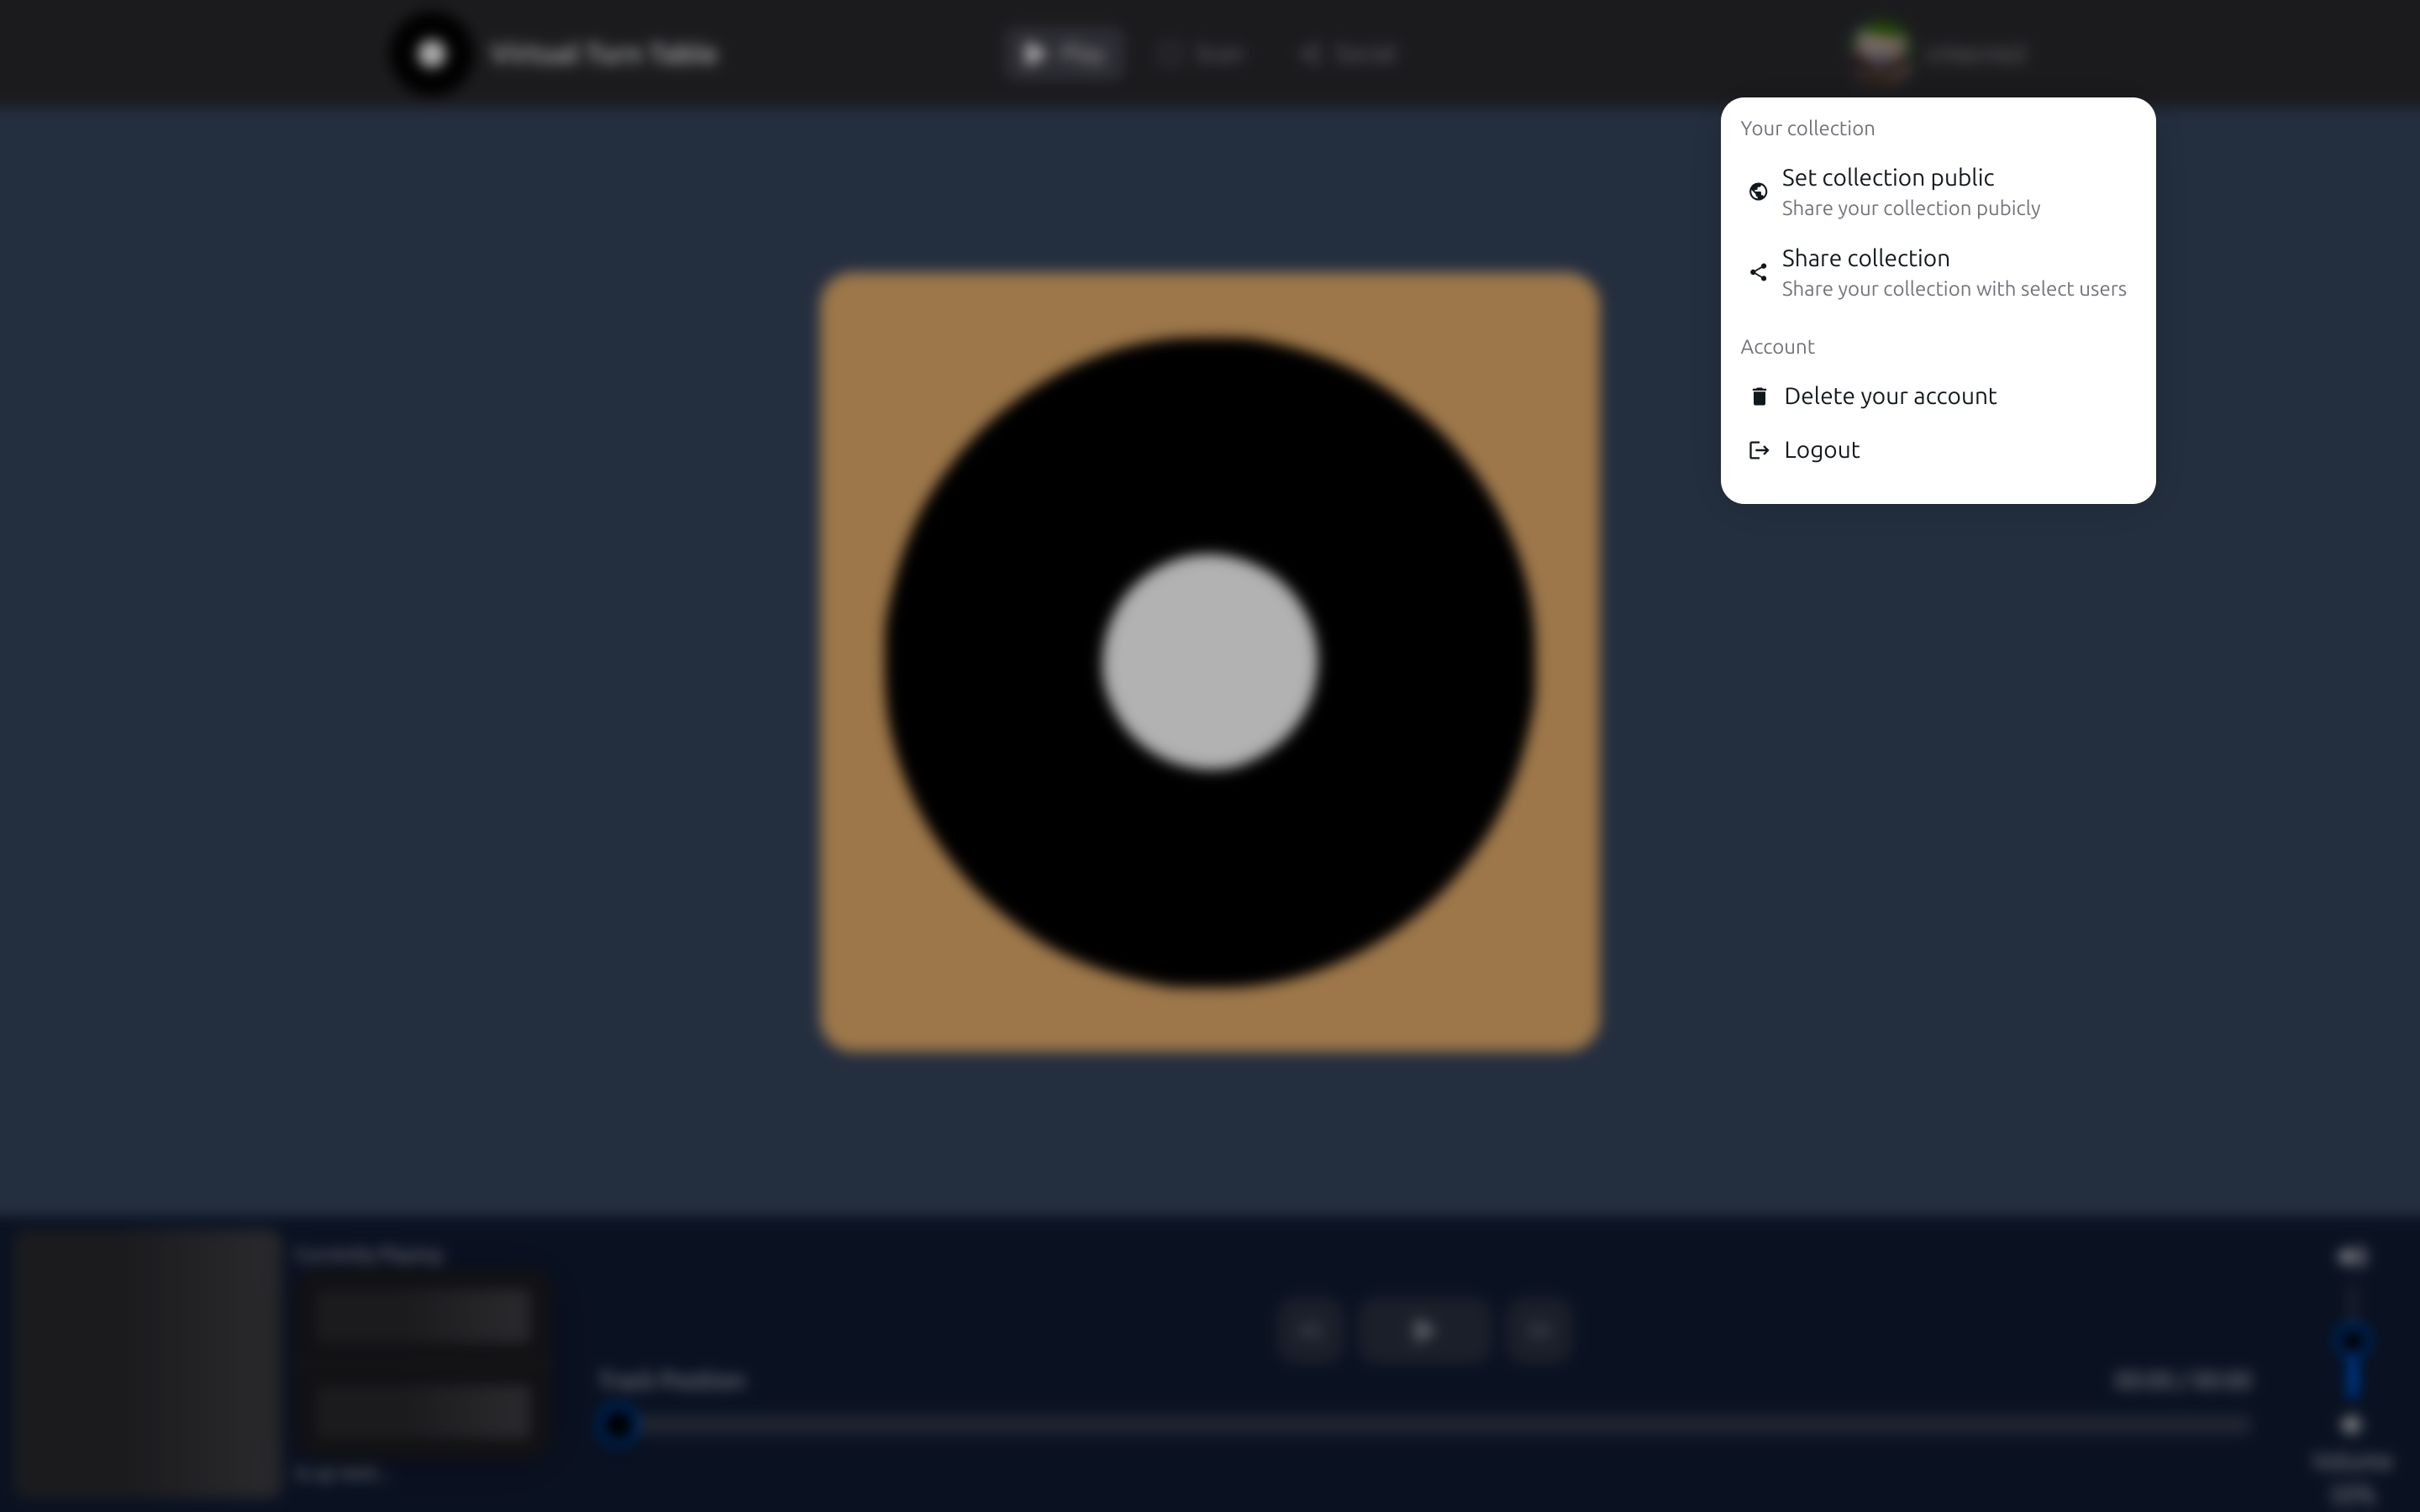
\includegraphics[width=0.8\textwidth]{figures/menu_open_screen.png}
    \caption{The user options menu opened from the navigation bar}
    \label{fig:user_options_menu}
\end{figure}

\subsubsection{Play Screen}
The play screen largely follows the initial design, consisting of three main sections: the track list, the controls, and a spinning vinyl animation. Music playback is handled by the Spotify Web Playback SDK, a client side JavaScript library that enables real-time control of Spotify playback within the browser. Actions such as changing tracks, skipping forward or backward, and pausing are executed by invoking the corresponding methods provided by the SDK.

\paragraph{Track List}
The track list displays all tracks from the currently active album, which is set on the scan screen. It serves as a selection menu of tracks, allowing users to choose a specific song for playback similarly to a music streaming service. The component is styled to fill up all vertical space between the navigation bar and scrolls vertically if the number of tracks exceeds the available space.

\paragraph{Controls}
The playback controls consist of buttons and sliders which users can interact with to effect audio playback. Clicking a button or adjusting a slider calls the relevant SDK methods, allowing users to play, pause, skip, or adjust volume. Album art and track information are displayed, so the currently playing track can be easily identified, these automatically update as the active song changes.
One feature from the original design was removed, the ability to scrub through the whole album rather than only the currently playing track. This was considered too complex to implement and added little to the user experience and so was excluded from the final implementation.

\paragraph{Spinning Vinyl}
To emulate the feel of a physical record player, an animated spinning vinyl graphic was implemented, featuring the album cover in the centre. Just as if this were a real record player, the vinyl rotates when music is playing and stops when paused. This was controlled by editing the rotation styling of the graphic.

A second animation was added to simulate the act of removing the vinyl from its sleeve when changing albums. This is meant to replicate the experience of removing a vinyl record from its sleeve and placing it on the turntable. This was done by animating the vinyl graphic to move to the side of the screen and then back to the centre with a new album cover.

\begin{figure} [H]
    \centering
    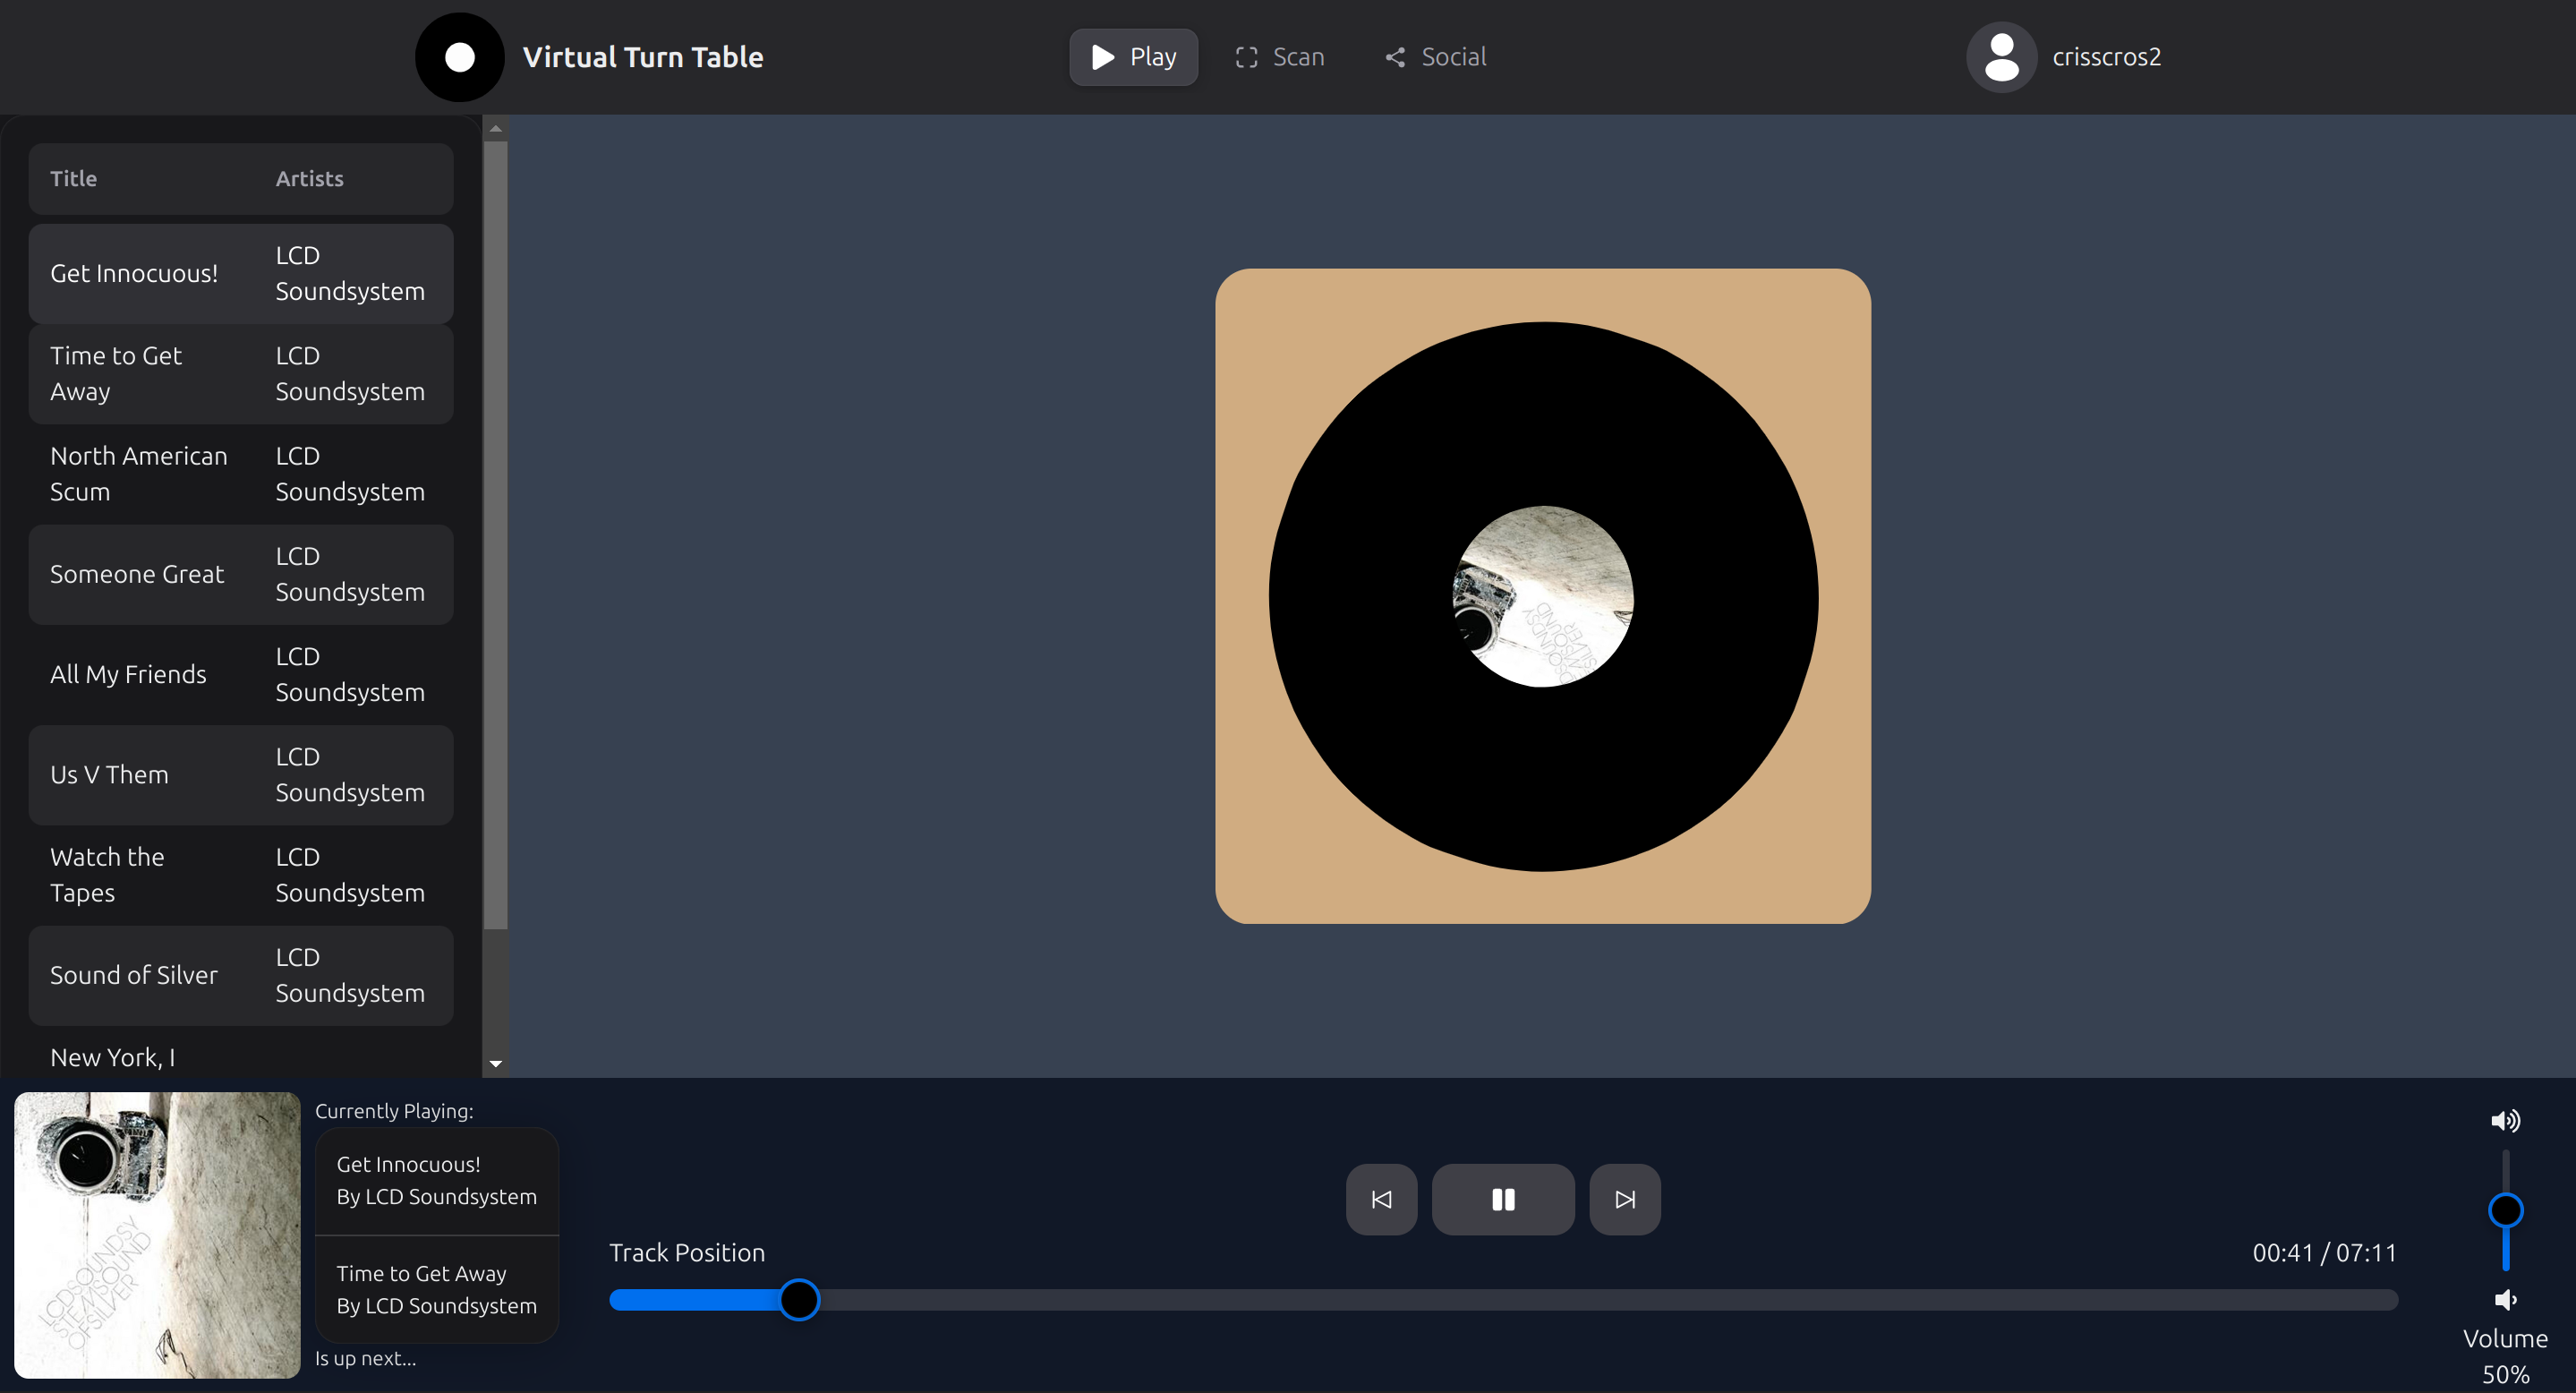
\includegraphics[width=0.8\textwidth]{figures/play_screen.png}
    \caption{The play screen of the application}
    \label{fig:play_screen}
\end{figure}

\subsubsection{Scan Screen}
The scan screen, though following the initial design as closely as possible, had to be changed during development as some issues with the original design became apparent during development. Similarly to the play screen it was also split into three main parts: the album confirmation sidebar, the scan section, and the album collection.

\paragraph{Album Confirmation Sidebar}
The album confirmation sidebar allowed the user to confirm the album that the identified album was correct. This presented an issue that was not addressed in the original design, how to handle incorrect album identifications To solve this, a second stage of the confirmation was introduced, using a separate scatter shot approach taken to present alternative matches, as shown in Figure~\ref{fig:album_confirmation_sidebar_incorrect}. In addition to this, the sidebar also acts as a method to display to the user the application is processing through the use of a loading animation where the identified album will appear. Once the user confirms the album selection the sidebar slides back to the side of the screen and the album is set as the active album.

\begin{figure}[H]
    \centering
    \begin{subfigure}[t]{0.3\textwidth}
        \centering
        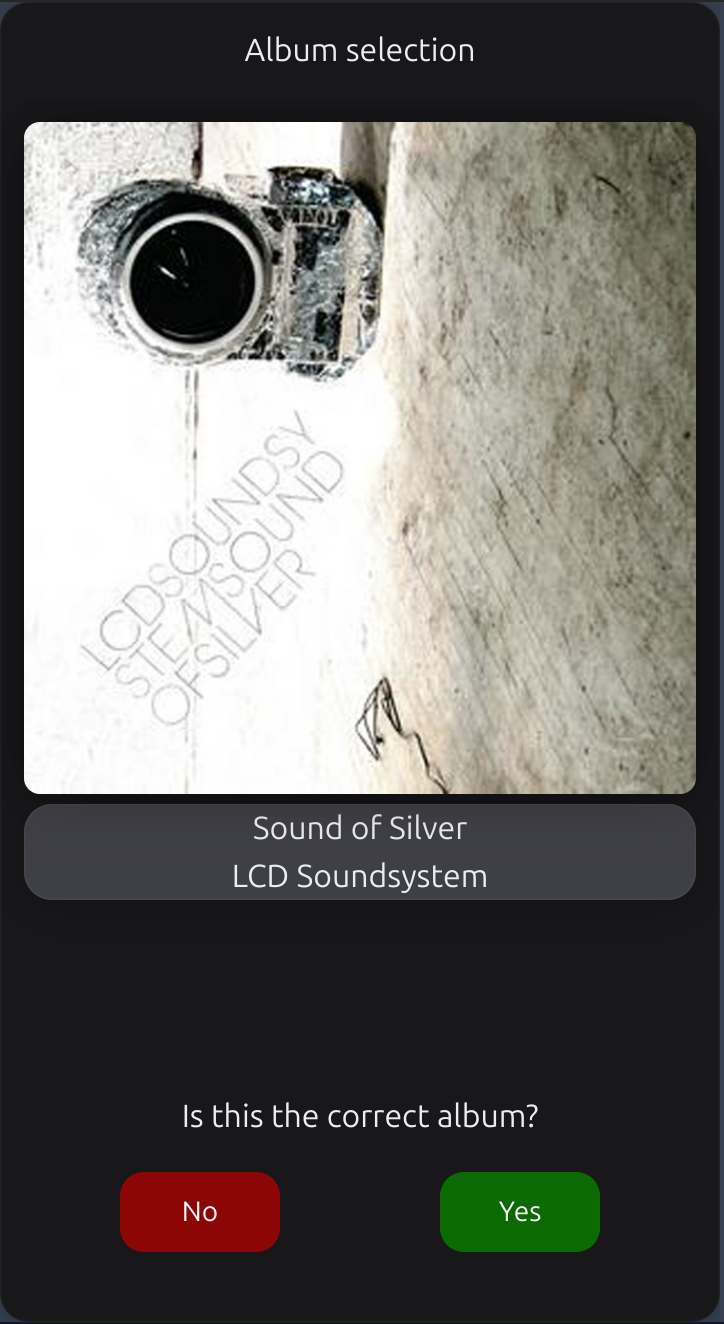
\includegraphics[width=0.8\textwidth]{figures/corrent_album_confirm.png}
        \caption{The album confirmation sidebar with the correct album guessed}
        \label{fig:album_confirmation_sidebar}
    \end{subfigure}
    \begin{subfigure}[t]{0.3\textwidth}
        \centering
        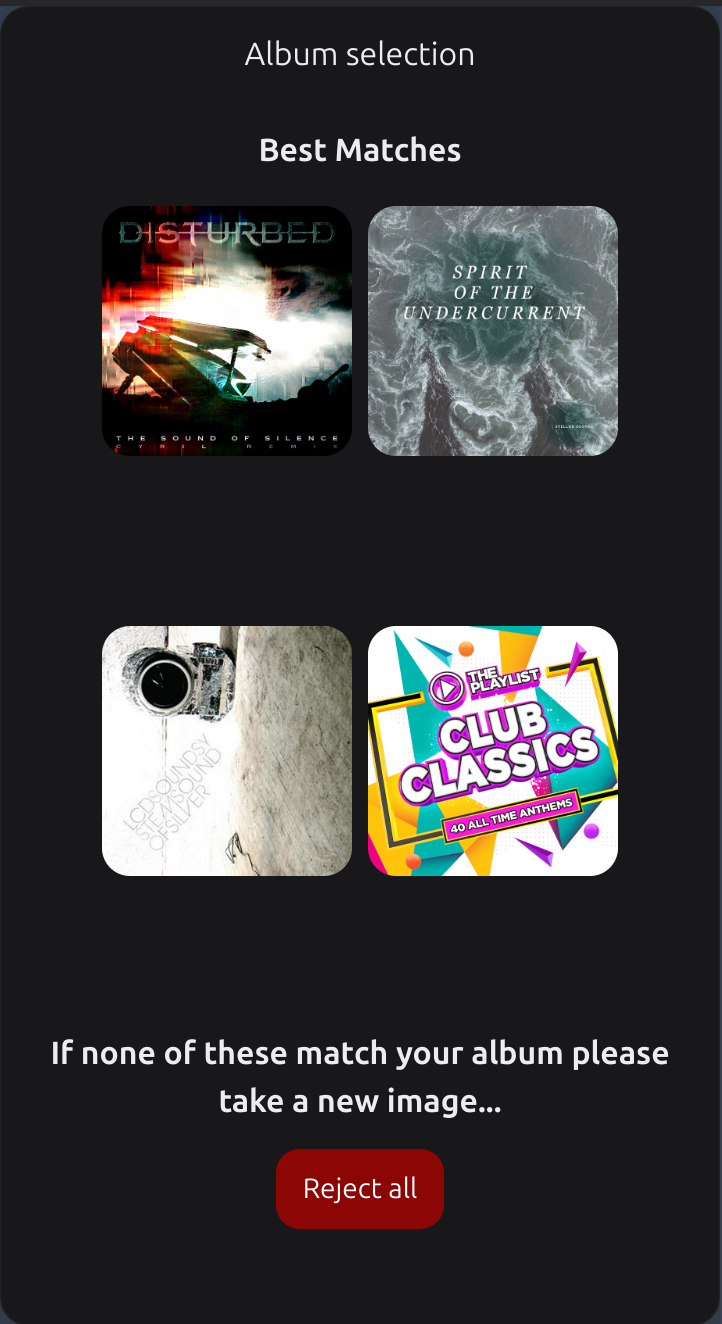
\includegraphics[width=0.8\textwidth]{figures/top_results_confirm.png}
        \caption{The album confirmation sidebar with the incorrect album guessed}
        \label{fig:album_confirmation_sidebar_incorrect}
    \end{subfigure}
\end{figure}

\paragraph{Scan Section}
Similarly to the confirmation sidebar an issue was identified in the scan section. The original design did not account for users who may not have a camera connected to their device. To solve this a file upload option was introduced, as seen in Figure~\ref{fig:upload_component}. If no cameras can be accessed by the browser, this option becomes the default. This was also useful for users who may not want to use their camera and so the option to upload an image is available to all users.

\begin{figure} [H]
    \centering
    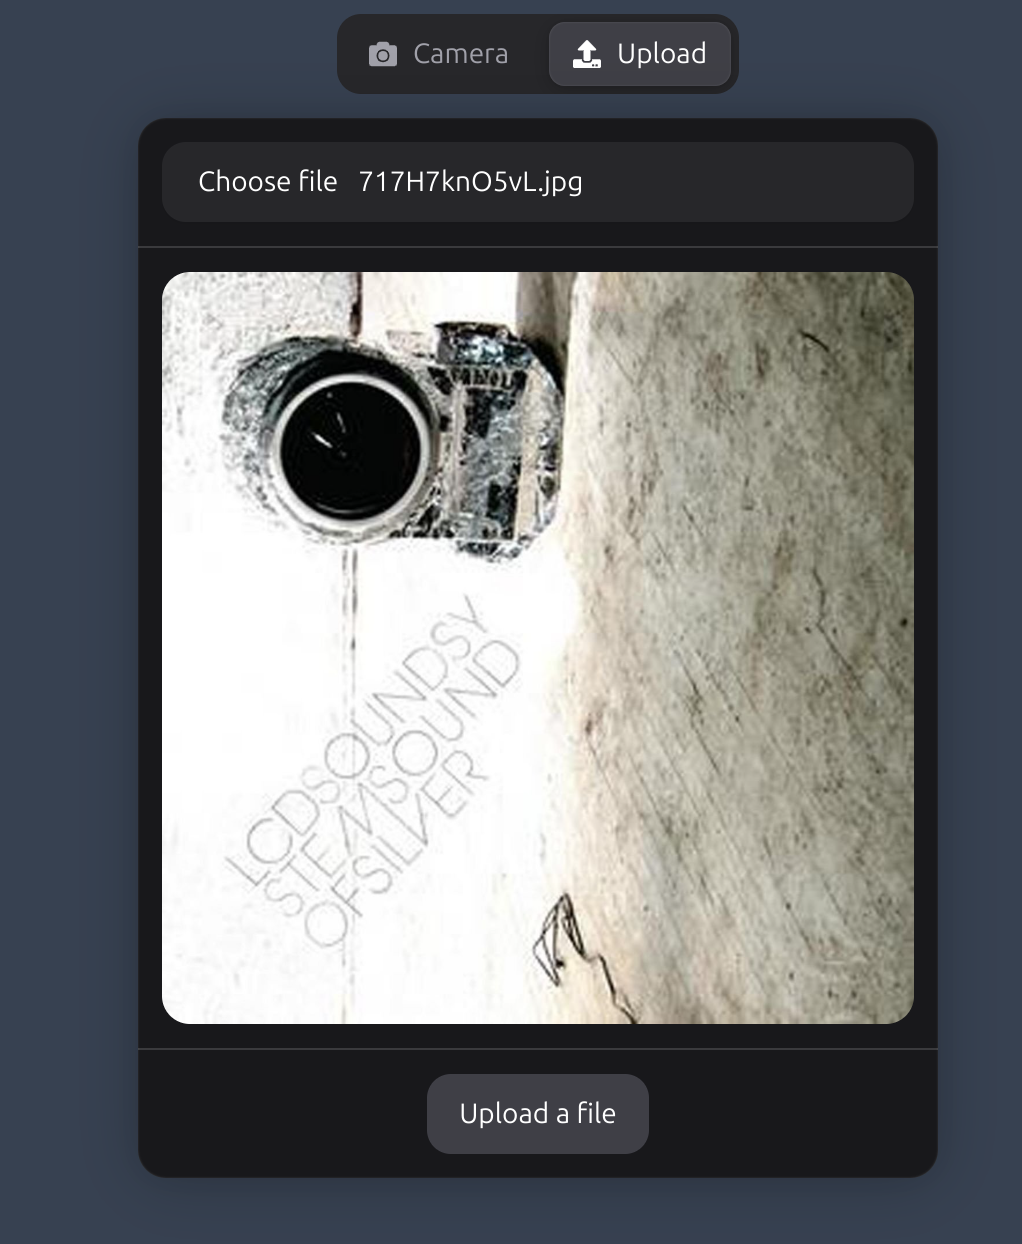
\includegraphics[width=0.4\textwidth]{figures/upload_component.png}
    \caption{The file upload component}
    \label{fig:upload_component}
\end{figure}

\paragraph{Album Collection}
This section remained mostly unchanged from the original design. The user's albums slide across the bottom of the screen allowing the user to select one by clicking on an album cover. When a user hovers over an album the sliding is paused and extra details of that album appear as a tooltip, such as the title and artist.
A feature that was added to the original design is the ability to look through the user's collection in a different format is also available by clicking the view all button. This opens a modal with all the user's albums in a view reminiscent of flicking through vinyl records in a record store, as seen in Figure~\ref{fig:collection_flick_through}.

\begin{figure} [H]
    \centering
    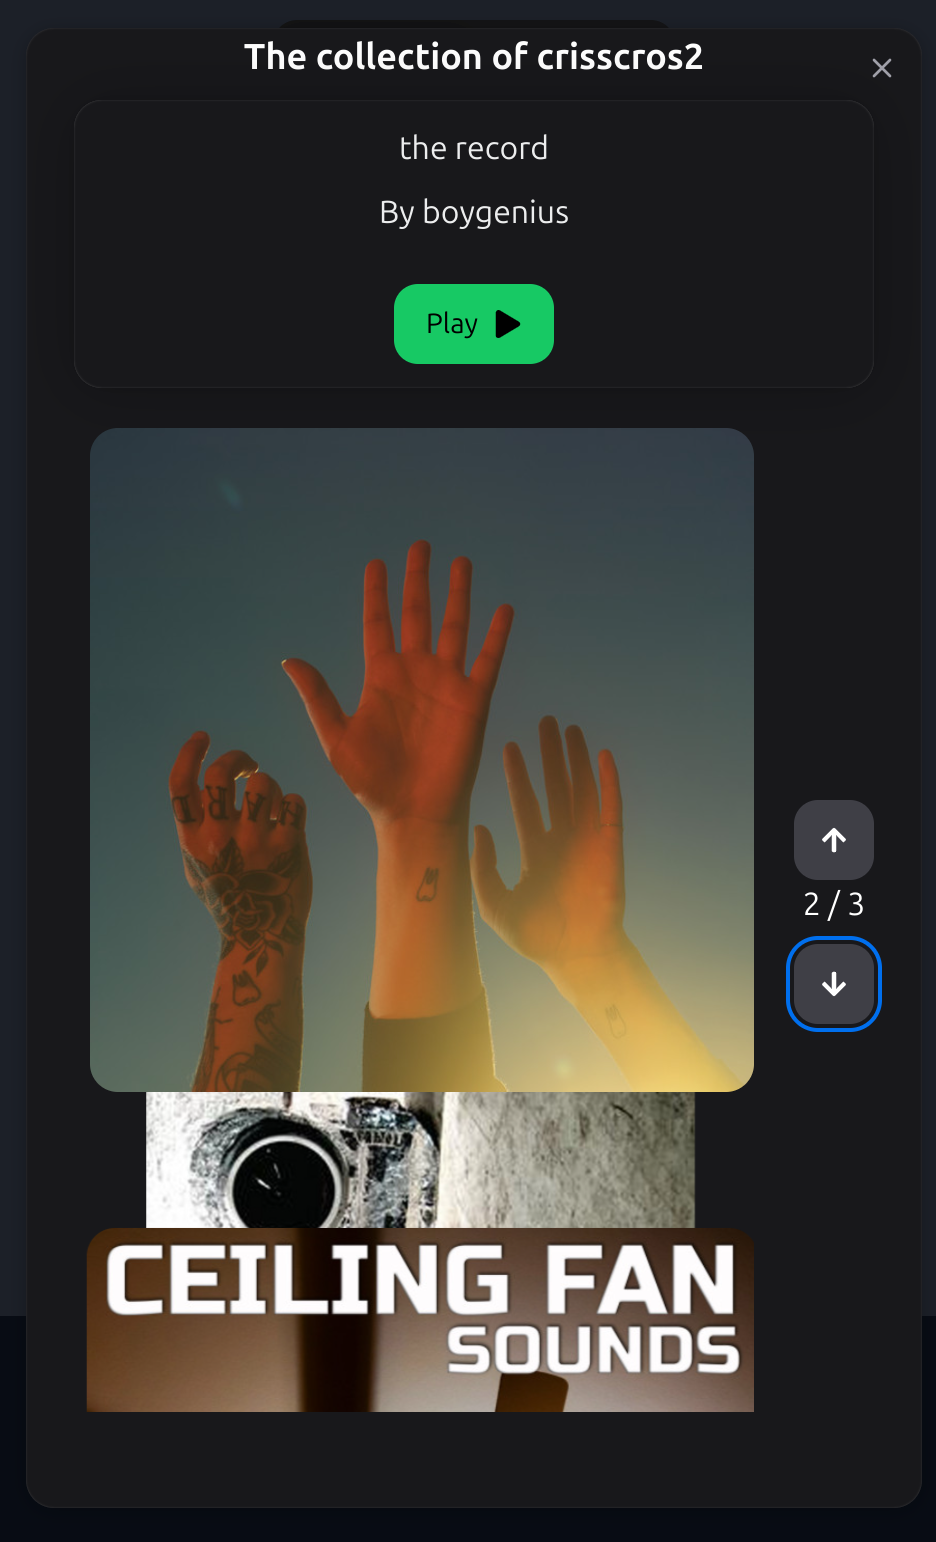
\includegraphics[width=0.3\textwidth]{figures/collection_flick_through.png}
    \caption{The view collection modal}
    \label{fig:collection_flick_through}
\end{figure}

\begin{figure} [H]
    \centering
    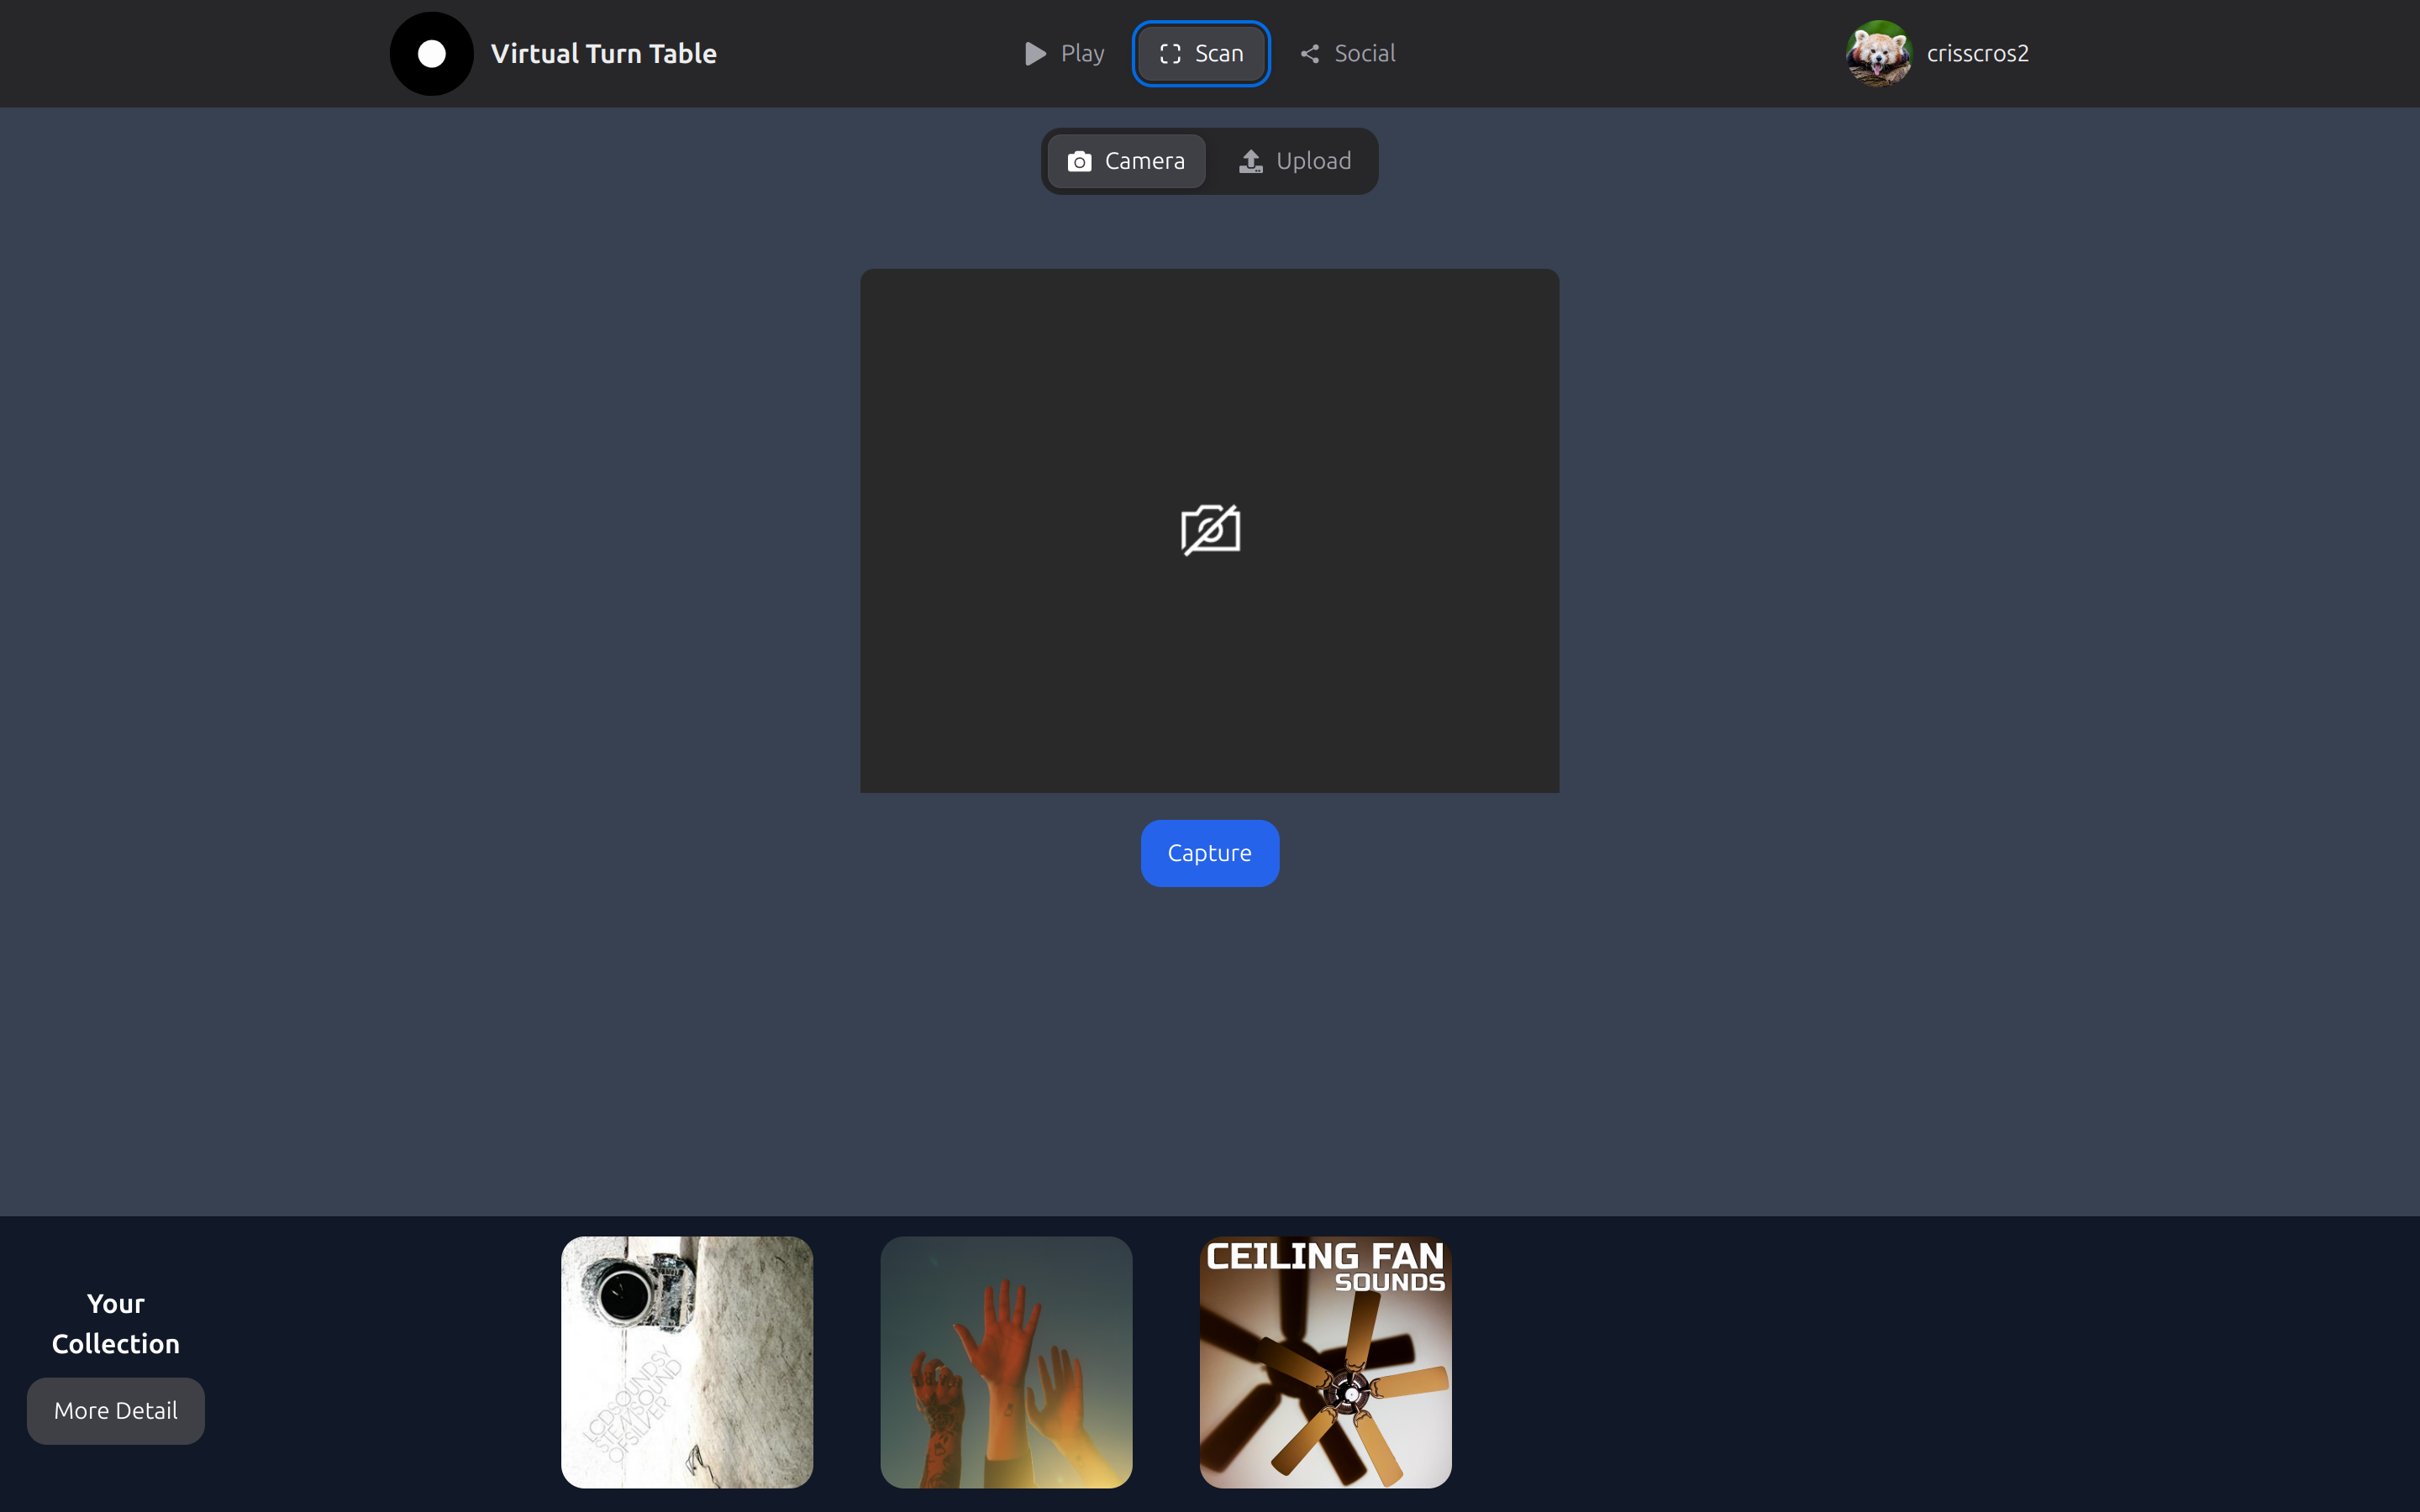
\includegraphics[width=0.8\textwidth]{figures/scan_screen.png}
    \caption{The scan screen of the application with the camera disabled}
    \label{fig:scan_screen}
\end{figure}

\subsubsection{Social Screen}
The social screen had the most significant changes from the original design. Initially, it was implemented as shown in Figure~\ref{fig:social_screen_mockup}, but this layout proved too cluttered, making it increasingly difficult to navigate larger collections and so a more compact design was needed.

The final design was inspired by the experience of flicking through vinyl records in a record store. Each user's collection is displayed within a grid, where albums pop up and down at random intervals. This approach allows a greater number of collections to be visible simultaneously without overwhelming the user.

To enhance usability further, additional collections can be loaded incrementally by clicking the Load More button at the bottom of the screen. Users can also explore collections in greater detail by selecting them. This means the user is presented with information as it is wanted which was a vast improvement over the original design which filled the screen with too much information for the user to process.

\begin{figure} [H]
    \centering
    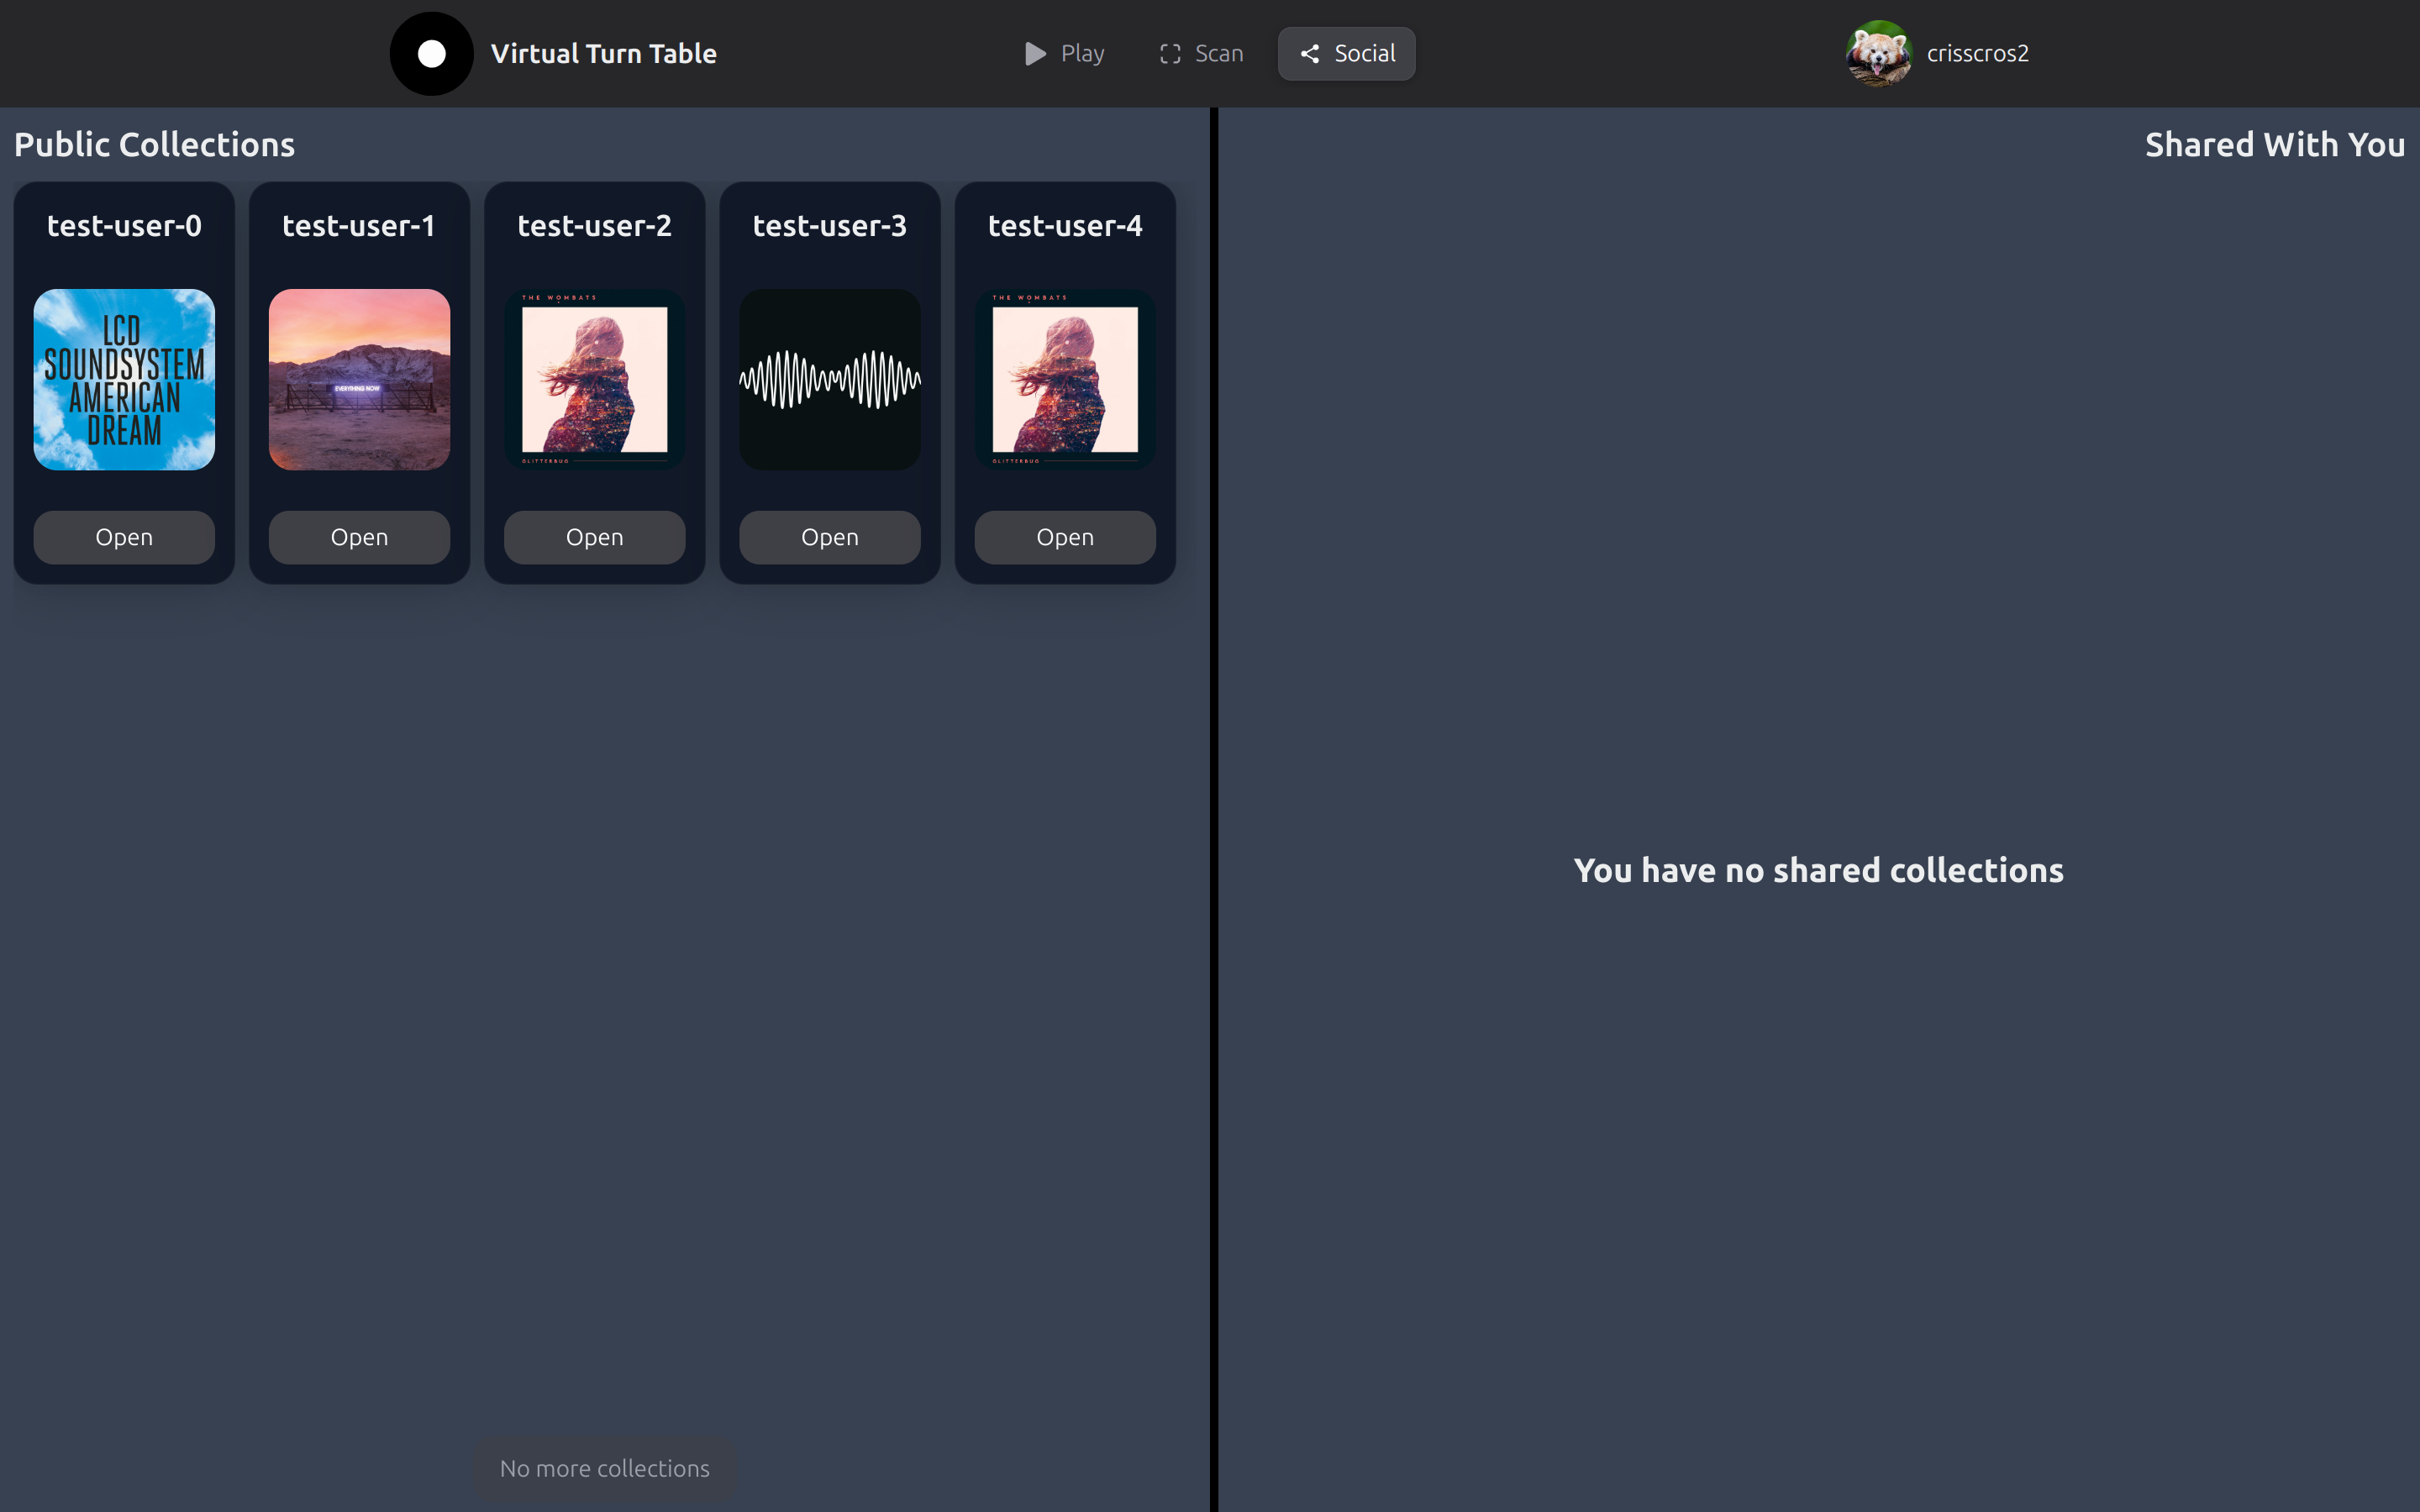
\includegraphics[width=0.8\textwidth]{figures/social_screen.png}
    \caption{The social screen of the application with five public albums and no shared albums}
    \label{fig:social screen}
\end{figure}

\subsection{Automated Testing}
Automated testing of the frontend was carried out using Vitest~\cite{Vitest}, a testing framework designed for projects built with the Vite build system. A test driven development (TDD) approach was adopted, where test cases were written for each component before the implementation is written. These tests defined the expected functionality of the component, ensuring that development aligned with predefined functionality. The minimum amount of code is then written to pass these tests and then further refactoring is made to the resulting component to improve it. In some cases, test cases themselves required refinement, as unexpected problems necessitated changes in approach for developing specific components. This approach ensured that components did in fact carry out the intended functionality and could be reliably tested in isolation.

The goal for automated testing was to achieve $95\%$ test coverage, which would ensure a high level of confidence in the application's functionality. To enforce this, a GitHub Action was configured to run tests on every pull request and push onto the main branch of the repository. The build process was set to fail if test coverage dropped below $95\%$ or if any test case failed ensuring these objectives were met.

\subsection{Containerisation}
Containerisation for the frontend involved creating a Docker image which contained a pre-built version of the frontend. On start this would serve the application via an exposed port that users could connect to.

The build of the application itself was straightforward once dependencies are installed. However, these dependencies are not required to be in the Docker image once the build is complete and since cloud storage has a cost associated with it the size of the image should be minimised. To achieve this a two stage build approach was employed.

\begin{description}
    \item[Build Stage] In this stage a base Node image is used to install all dependencies and then build the application.
    \item[Production Stage] In this stage the built application is copied from the build stage into a new image. All data not copied from the build stage is left behind, resulting in a much smaller image. This is the image that is then served.
\end{description}

\subsection{Dependency Management}
Frontend dependencies were managed using Node Package Manager (NPM). As new dependencies were installed, a JSON file within the repository was updated to record the package names and their versions. From this file any developer using NPM could install all required dependencies with a single command.

To maintain up-to-date and secure dependencies, Dependabot, a service provided by GitHub, was integrated into the repository. Dependabot automatically scanned the dependency file at predefined intervals (e.g. weekly or monthly) and generated pull requests for available updates. This approach ensured that security vulnerabilities were patched and keeps all dependencies at their latest versions, so the application would not run using deprecated dependencies.

The automated testing provided a mechanism to verify whether updated dependencies introduced breaking changes without manual intervention.

\subsection{Challenges}
\paragraph{Environment}
The biggest challenge in frontend development was managing environment variables across different deployment environments. For instance, the BFF URL varied between the development environment, the Docker Compose environment, and the production environment.

This issue was partially solved through the use of dotenv files, which allowed environment variables to be defined in a file and automatically loaded into the application. However, since these files often contained sensitive information, such as API secret keys, committing to version control was not an option and so instead the files had to be managed manually. Despite this limitation, once the dotenv files were properly set up, the approach functioned reliably across deployments.

\paragraph{Spotify API Changes}
Midway through development, Spotify updated their authentication flow to require HTTPS for redirect URLs, disabling non-HTTPS redirects~\cite{spotifyredirects}. The cloud deployment was unaffected, as it already used HTTPS. However, the development environment did not, breaking the authentication flow when running locally. Fortunately, there was an easy fix, the services were just launched using self-signed SSL certificates. Though the impact on the project was small this change highlights the risks of relying on external services and the potential for breaking changes.

\paragraph{Maintaining State Between Refreshes}
The local state of the frontend is managed through variables that are reset upon page refreshes. As a result, if a user refreshes the page or closes the browser and reopens it, the session is lost, requiring them to go through the process of logging in and selecting or scanning an album. This issue was solved via state persistence, implemented using the browser's local storage. When the application initialises, it attempts to retrieve stored session data. If valid data is found, the session is restored, allowing the user to continue from where they left off. Meaning if a user refreshes the page while listening to an album, they are returned to the play screen with the same album and song still playing.

\section{Backend}~\label{sec:backend-development}
\subsection{Implementation}
Each backend service followed a similar implementation structure, consisting of a FastAPI application responsible for serving API endpoints. Depending on the service's functionality, it could also establish WebSocket connections or interact with a database.

All three services included two basic endpoints:
\begin{description}
    \item[Health Check:] A health check endpoint to monitor service availability.
    \item[Docs Redirect:] A redirection endpoint leading to the automatically generated API documentation (removed in the deployed version).
\end{description}

In order to better organise the API, each service was structured using routers to categorise endpoints into logical sections, such as authentication or user data retrieval. This modular approach improved API organisation, making it easier to understand and use.

\subsubsection{BFF}
The Backend for Frontend (BFF) service was structured into five distinct routers, each responsible for a specific aspect of the application:

\begin{description}
    \item[Music Router:] Handles all endpoints related to music playback and retrieving album or song data.
    \item[User Router:] Manages user-related endpoints, including user data retrieval and updates.
    \item[Image Search Router:] Facilitates communication with the image-to-album service, handling album identification from uploaded images.
    \item[Authentication Router:] Manages user authentication, including login and token validation.
    \item[Social Router:] Handles endpoints related to the social functionality, such as collection sharing and retrieving shared collections.
\end{description}

Additionally, the BFF manages the WebSocket functionality for the notification system. When a user logs in, a WebSocket connection is established between the frontend and the BFF. If a collection is shared with the user, the BFF asynchronously sends a notification via the WebSocket connection, prompting the frontend to display the new notification to the user.

\subsubsection{User Data Service}
The User Data Service was the most complex of the three backend services, as it required direct interaction with a database. SQLAlchemy was used as the Object-Relational Mapping tool to manage database interactions, with each database table defined as a model in the code.

The service was structured into two primary routers:

\begin{description}
    \item[User Router:] Handles all endpoints related to individual users.
    \item[Social Router:] Manages endpoints related to social functionality, including collection sharing and retrieval.
\end{description}

To ensure data is not lost during database schema changes Alembic, a database migration tool was used. This automatically generated migration files, which could be executed to update the database schema while preserving existing data. Although this was not a critical concern during development, since no real user data was stored, such a system would be important in a production environment, where data persistence must be maintained across schema updates.

\subsubsection{Image To Album Service}
The Image-to-Album Service was the simplest of the three backend services, consisting of only two routers, each containing a single endpoint:

\begin{description}
    \item[Image Processing Router:] Handles the conversion of an uploaded image into a predicted album match.
    \item[Album Retrieval Router:] Retrieves the corresponding Spotify album ID based on the predicted album match.
\end{description}

This service was completely stateless, and as such it did not require persistent data storage between requests.

The image processing functionality was implemented using the best guess functionality of the Google Reverse Image Search API. This guess would then be run through the Spotify search API which would return an album which would be displayed to the user. The scatter shot approach used separate data from the same reverse image search. It would instead look at the websites matches to the image were found on and use the title of the page as a search term. This proved to be effective because music albums are often the subject of reviews and sales pages which would contain the album title.



\subsubsection{Security}~\label{sec:backend-security}
Security measures were implemented differently across the three backend services to ensure proper control over data access.

For the User Data Service and Image-to-Album Service, security was enforced by middleware that rejected all requests not originating from the BFF service. This ensured that only authenticated and validated requests from the BFF could interact with these services.

The BFF required a more complex security approach, as it had to handle requests from external users. To authenticate users, JSON Web Tokens (JWTs) were used, which are common in web applications~\cite{9320801}. When a user logs in via Spotify, the frontend sends that token to the backend. If the token is valid, the backend issues a JWT formed from the given token and the user's username, this is then included in the headers of subsequent requests to the BFF.

This token-based authentication ensures that that users can only access their own data, and that requests without a valid JWT are rejected, preventing unauthorized access.

\subsection{Automated Testing}
Automated testing for the backend was carried out using the Pytest library~\cite{PyTest}, which allows for the creation of custom test fixtures to set up and tear down the environment for each test, including managing the database state. FastAPI provides a test client which was utilised to simulate calls to endpoints to be tested as if the endpoints were being called by an actual client.

Extensive use of mocking was necessary for simulating external API calls. This was especially important in the BFF service, which made numerous calls to the other two backend services. Mocking ensured that each service could be tested in isolation without requiring live responses from the other services and  external APIs, making the testing process more reliable and efficient.

\subsection{Containerisation}
Each of the three backend services was containerised using an Alpine Linux image with Python pre-installed. Alpine Linux was chosen due to its minimal footprint, making it one of the smallest available Linux distributions. There are also security benefits to this approach, as the reduced number of features in Alpine Linux means there are fewer potential vulnerabilities to exploit.

Unlike the frontend, where dependencies are only needed during the build process, the backend dependencies must be present at runtime for the services to function correctly. As a result, a multi-stage build was not used. Instead, dependencies were installed in the same stage as the application files were copied into the container image, ensuring that all required packages were available when the service was deployed. This disadvantage of this approach is that the image size is larger, but this is unavoidable due to the nature of the backend services.

\subsection{Dependency Management}
Unlike Node applications, Python does not have a standardised dependency management system, there are multiple tools such as Pipenv and Poetry which can be used. For simplicity, the solution chosen for this project was a requirements.txt file, which lists all dependencies using semantic versioning. This approach allows dependencies to be installed using pip, the most widely used Python package manager, with a single command.

Dependency updates were managed similarly to the frontend. Dependabot was configured to scan the requirements.txt file at regular intervals, generating pull requests for available updates. These updates followed the same schedule as frontend dependencies, ensuring that the dependencies were kept up to date and security vulnerabilities were patched as soon as possible.

\section{Code Quality}~\label{sec:code-quality}
Code quality standards were maintained during development through the use of pre-commit hooks and GitHub Actions. Pre-commit hooks were configured to run linters and formatters before code was committed to the repository. This ensured that potential issues were identified early, preventing poor quality code from making it into the repository. This approach was particularly valuable since the project was developed by a single developer, and so there was no code review process to catch mistakes.

In addition to the pre-commit hooks, automated tests and security scans were executed every time a pull request was created or a commit was pushed to the main branch of the repository. While these checks could have been integrated into the pre-commit hooks, this was avoided due to the execution time of the tests, which would have led to a tedious development process. Instead, the tests were run on GitHub servers, leveraging parallel execution to reduce the overall testing time.

\chapter{Deployment}~\label{cha:deployment}
Once development was complete, the application had to be deployed to be accessible to users. This involved configuring two ways to run the application: locally, using Docker Compose and on the web, using a cloud hosting service
TODO: Add more content here.

\section{Docker Compose}
Docker Compose is a container orchestrator that allows multiple containers to be run together on one system in unison [TODO: Add ref here]. A single command can be used to both build and run the containers. The overall structure of the deployment is defined in a single file which defines which services are run and how. This includes defining environment variables, volumes, and ports to be exposed. An important part is also defining which endpoint can be called as a health check which allows the orchestrator to determine if the service is running correctly. From this we can define dependencies between the services to determine start order so that the application can be run correctly.
% TODO: Add More

\section{On the web}
The web deployment was done using Google Cloud Run. A configuration can be pointed to the Dockerfile in the repository and, once triggered by an event on the repository, will build the image and deploy it to the web. It provides a URL and handles the complexities of hosting such as spinning up instances when needed and shutting them down when not in use.

The intention was for a build to be conducted and deployed after each push to the main branch, assuming every push passes all scans and tests. This, however, was deemed to be excessive for this application and so a tag mechanism was implemented, so builds are only triggered when a new tag is pushed to the repository.

This service, however, comes at a monetary cost as this is an infrastructure as a service (IaaS) model. Higher usage would result in higher costs especially for the storage of the Docker image after it is built on the cloud servers. For this project the free tier proved to be sufficient but if the application were to be used more widely costs would need to be considered.

\chapter{Evaluation}~\label{cha:evaluation}
Once the application was deployed, it had to be determined if it met the requirements set out in the design phase. The tests set out in Section~\ref{sec:test-design} were carried out to do this.

\section{Primary Features}
These tests relate to the two primary feature tests in Section~\ref{sec:test-design}. As these features were fundamental to the application's core functionality, their implementation was critical in determining whether the project succeeded.

\subsection{Album Scanning}
The album scanning mechanism consisted of two separate APIs, and the evaluation focuses on the accuracy of these two APIs and the effectiveness of the two methods used to identify albums, namely, using either the best guess from reverse image search results or extracted website titles.

Fifteen albums were used to conduct the evaluation. For each album six manipulated images were used, as shown in Table~\ref{tab:image-evaluation-examples}.
\ifshowappendix
Each used album is listed in Appendix~\ref{apd:test_albums}.
\fi

\begin{table} [H]
    \centering
    \renewcommand{\arraystretch}{1.5} % Adjust row height
    \setlength{\tabcolsep}{10pt}      % Adjust column spacing

    \begin{subtable}{0.48\textwidth}
        \centering
        \begin{tabular}{|m{2.5cm}|m{2.5cm}|}
            \hline
            \textbf{Image Type} & \textbf{Example} \\
            \hline
 Normal & 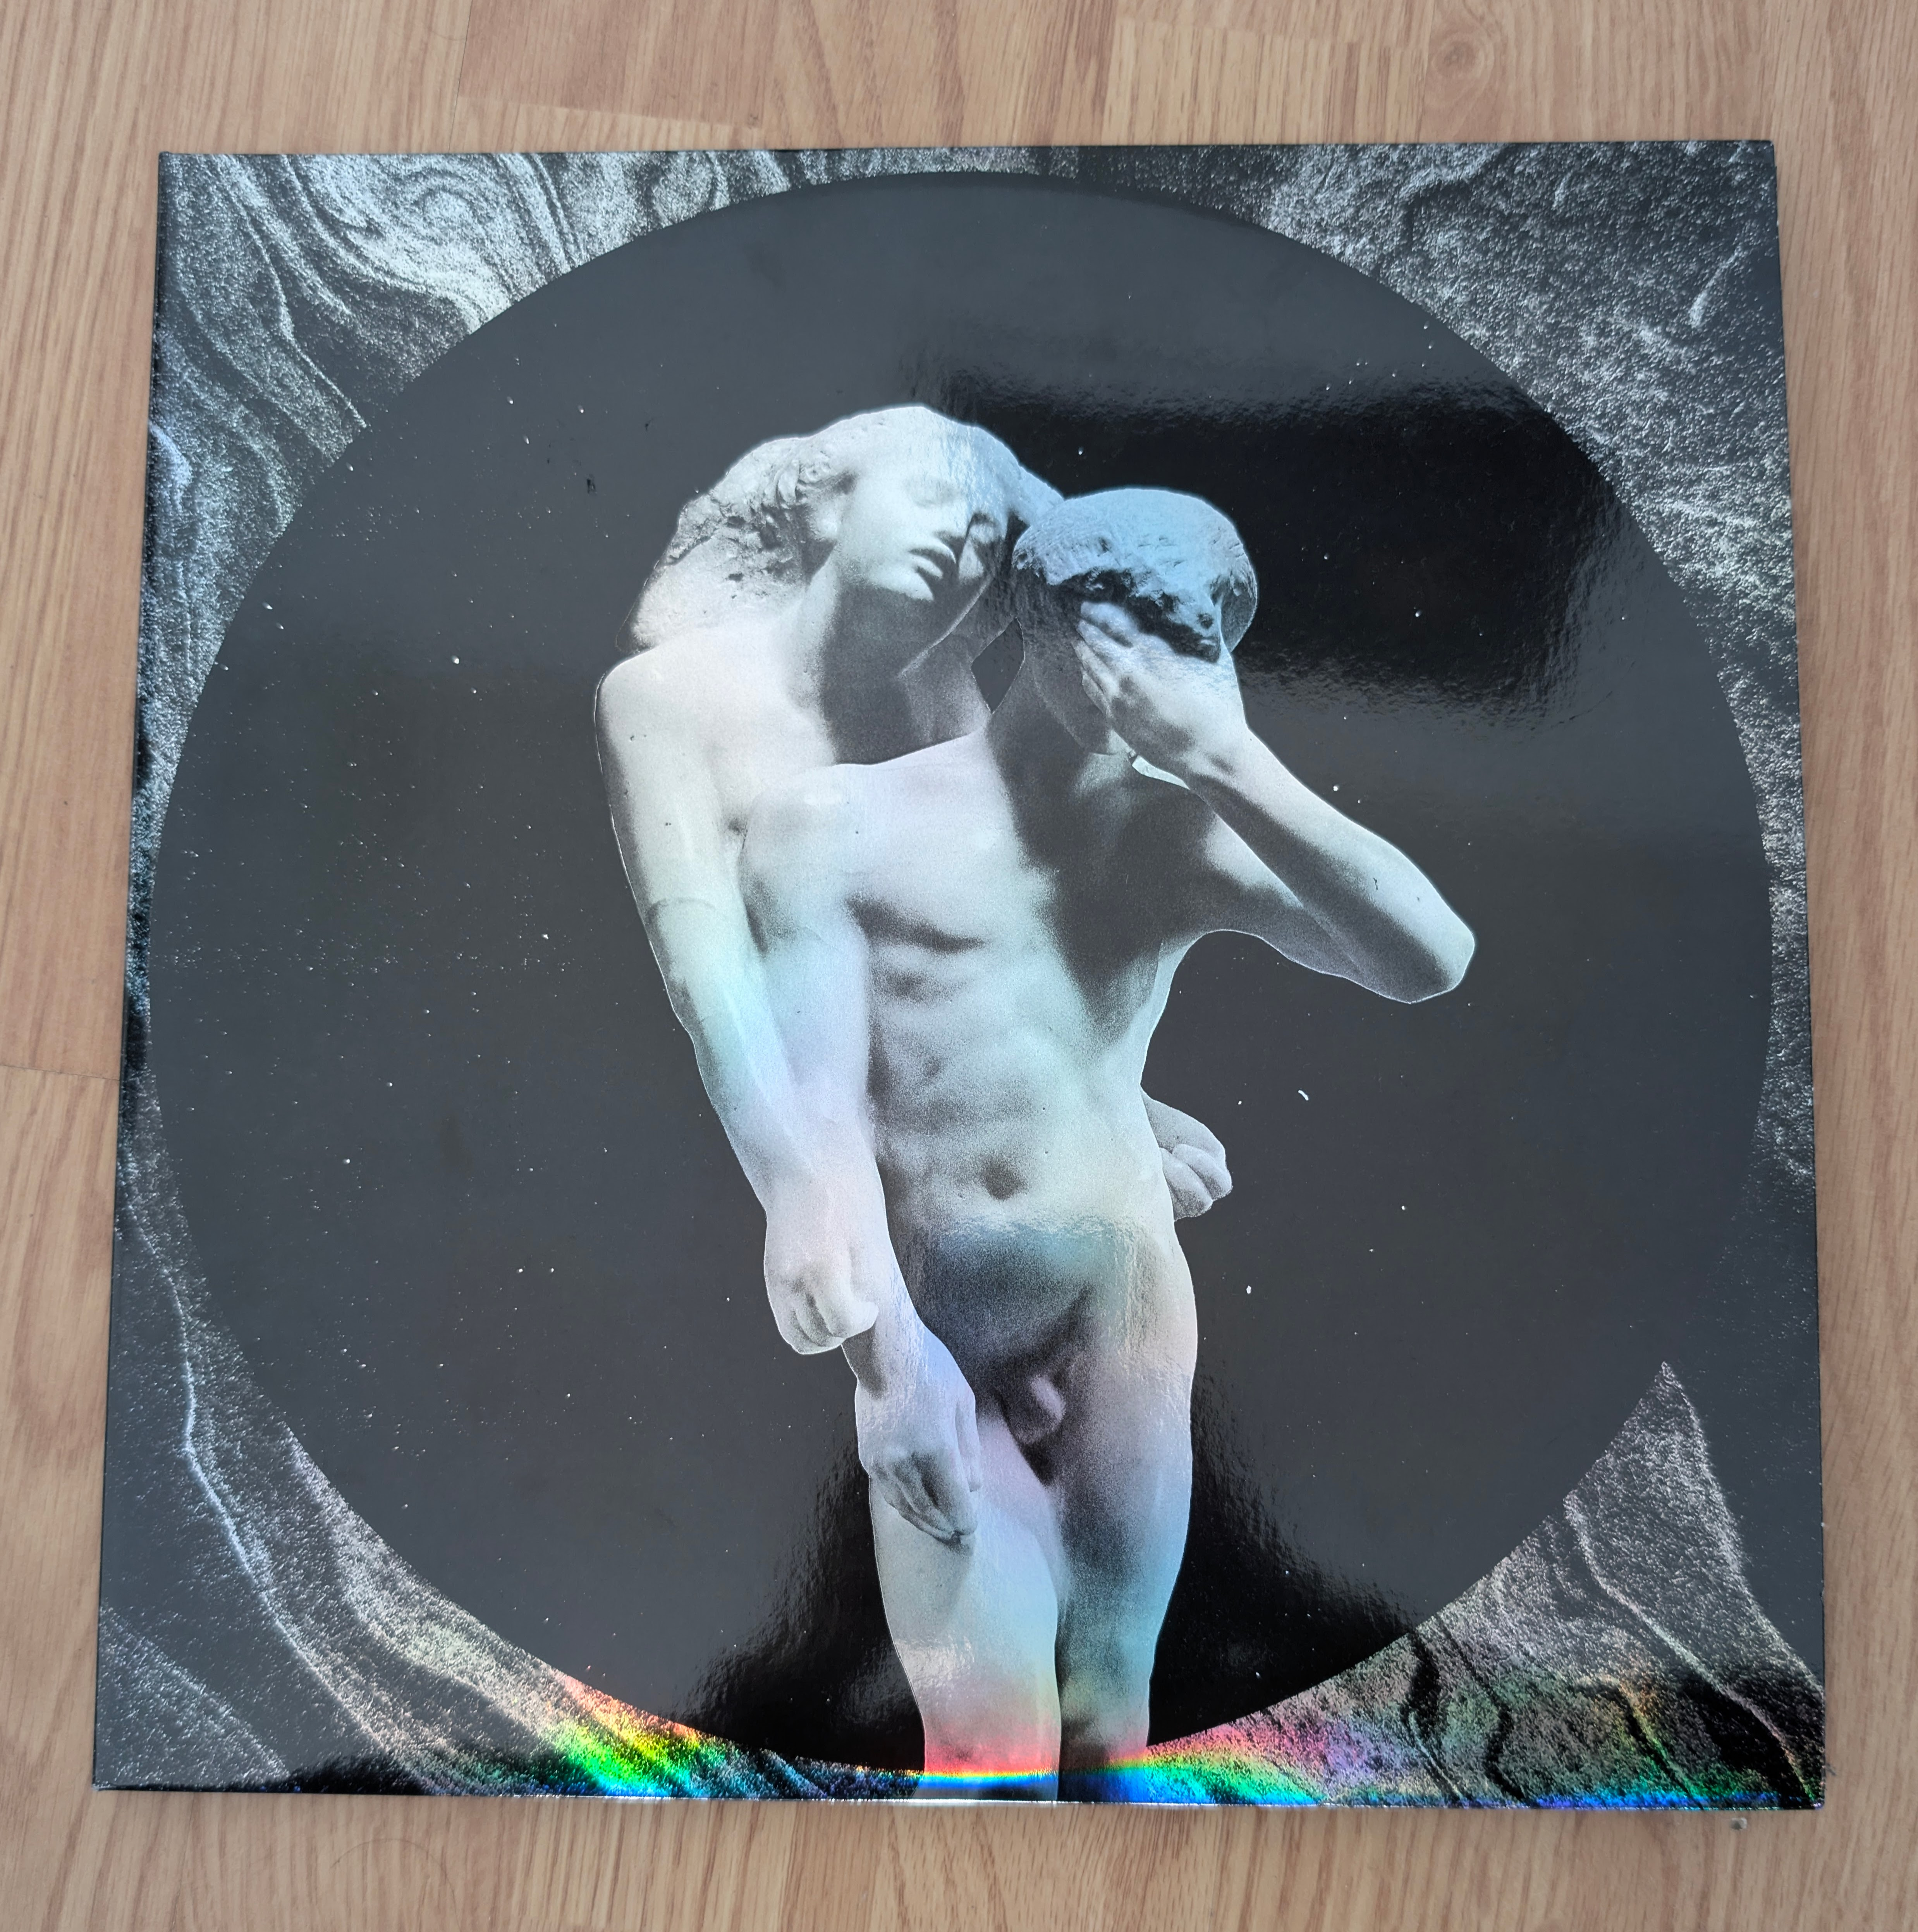
\includegraphics[width=2.5cm]{figures/test_albums/Reflektor.jpg} \\
            \hline
            Rotated $90$\textdegree & 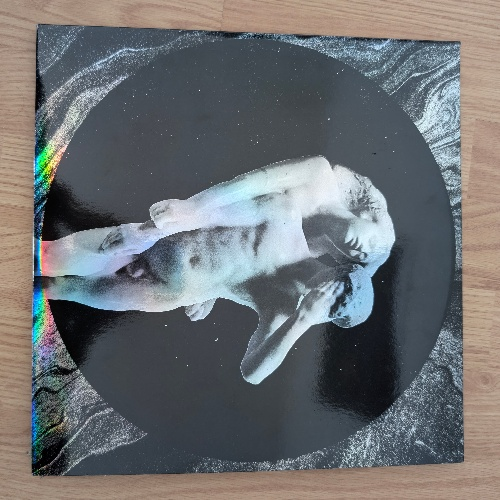
\includegraphics[width=2.5cm]{figures/test_albums/Reflektor_Rotated - 90.jpg} \\
            \hline
            Rotated $180$\textdegree & 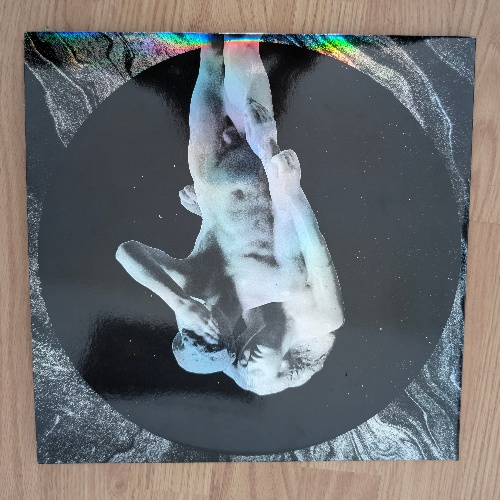
\includegraphics[width=2.5cm]{figures/test_albums/Reflektor_Rotated - 180.jpg} \\
            \hline
        \end{tabular}
    \end{subtable}
    \hfill
    \begin{subtable}{0.48\textwidth}
        \centering
        \begin{tabular}{|m{2.5cm}|m{2.5cm}|}
            \hline
            \textbf{Image Type} & \textbf{Example} \\
            \hline
            Rotated $270$\textdegree & 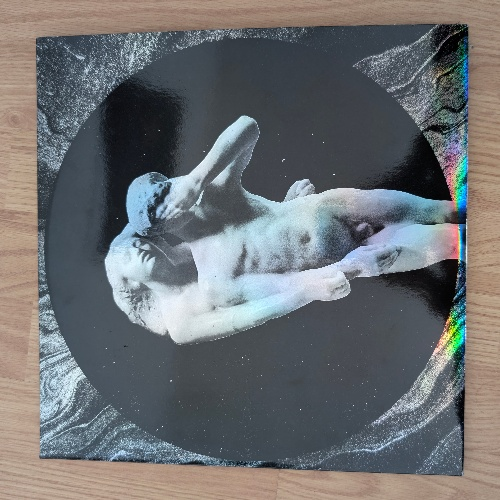
\includegraphics[width=2.5cm]{figures/test_albums/Reflektor_Rotated - 270.jpg} \\
            \hline
            Blurred & 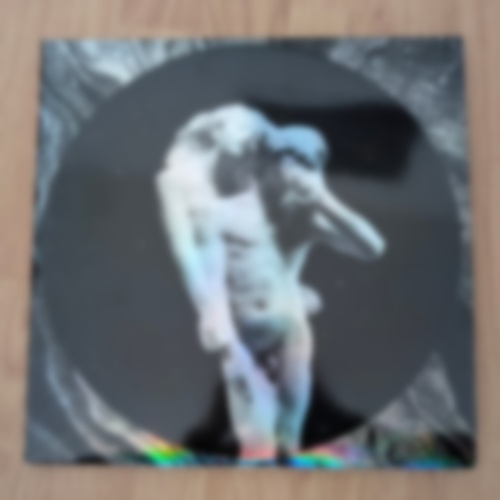
\includegraphics[width=2.5cm]{figures/test_albums/Reflektor_Blurred.jpg} \\
            \hline
            Scaled Down & 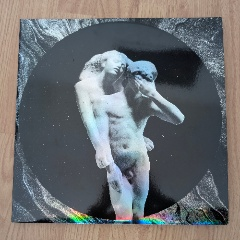
\includegraphics[width=2.5cm]{figures/test_albums/Reflektor_Scaled.jpg} \\
            \hline
        \end{tabular}
    \end{subtable}

    \caption{Example images used in the evaluation}
    \label{tab:image-evaluation-examples}
\end{table}

Self-taken images were preferred to ensure that the test cases were more representative of authentic user-uploaded images. This is opposed to using images already present on the Internet, which could be pre-indexed by search engines.

The criteria for a pass were defined as follows:
\begin{itemize}
    \item For reverse image search, a result was considered correct if the exact album name appeared in the returned results.
    \item For the Spotify search, a result was deemed correct if the correct album was returned.
\end{itemize}

\subsubsection{Results}
The results are split into two sets:
\begin{itemize}
    \item Reverse Image Search Accuracy – Displayed in Figure~\ref{fig:album-scanning-results-ris}, this dataset evaluates the accuracy of the Google Reverse Image Search API. While this API functions as a black box, as the application cannot affect its inner workings, evaluating its accuracy in practice is still valuable.
    \item Spotify Search Accuracy – Displayed in Figure~\ref{fig:album-scanning-results-spotify}, this dataset evaluates the accuracy of the Spotify Search API, considering only cases where the reverse image search correctly identified the album so the accuracy of the Spotify search could be isolated from the accuracy of the reverse image search.
\end{itemize}

\begin{figure} [H]
    \centering
    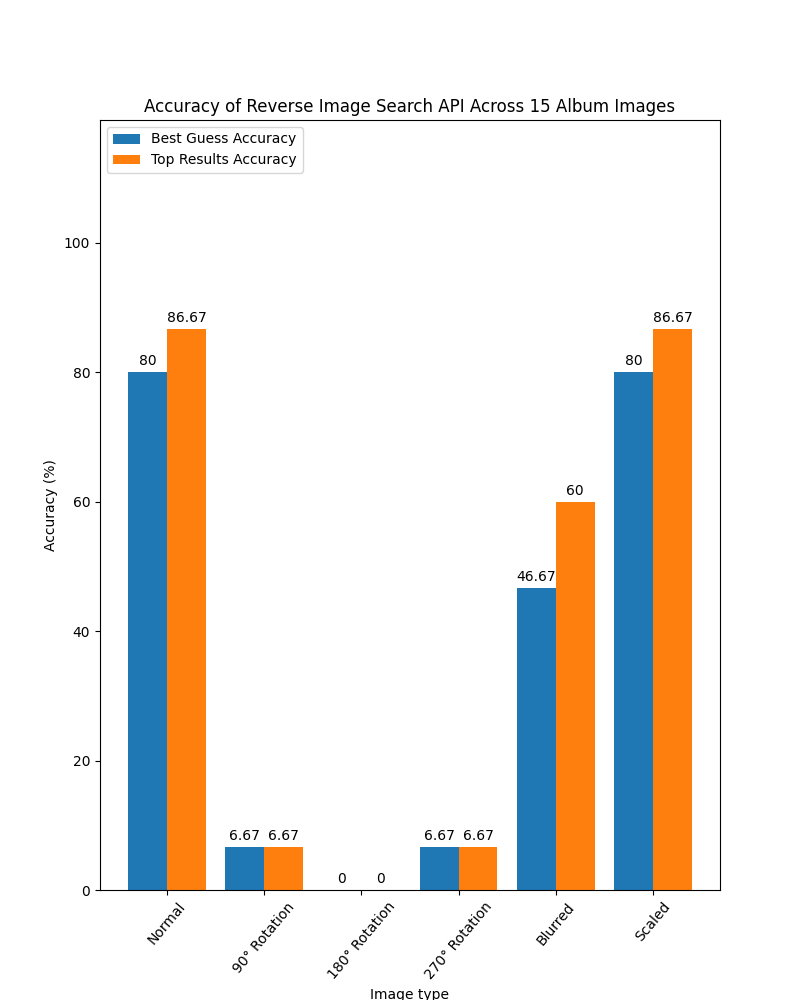
\includegraphics[width=0.65\textwidth]{figures/evaluation_graphs_ris.png}
    \caption{Accuracy of Reverse Image Search}
    \label{fig:album-scanning-results-ris}
\end{figure}

The results from the reverse image search did not meet expectations. While an accuracy of $95\%$ was targeted, the measured accuracy for images with no modification was significantly lower:
\begin{itemize}
    \item $80\%$ ($12$ out of $15$) accuracy when using the best guess from the reverse image search results.
    \item $86.67\%$ ($13$ out of $15$) accuracy when using website titles extracted from the search results.
\end{itemize}

Performance was particularly poor for rotated images, with only albums that had rotated artwork being correctly identified. The two examples of this in the test dataset are shown in Figures~\ref{fig:sos_rotated_90} and~\ref{fig:tih_rotated_270}.

\begin{figure} [H]
    \captionsetup{justification=centering}
    \centering
    \begin{subfigure}[t]{0.45\textwidth}
        \centering
        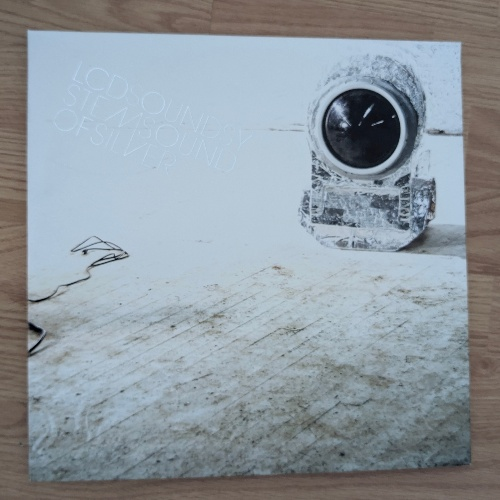
\includegraphics[width=0.45\textwidth]{figures/test_albums/Sound_Of_Silver_Rotated - 90.jpg}
        \caption{The only correct result for 90° rotation}
        \label{fig:sos_rotated_90}
    \end{subfigure}
    \begin{subfigure}[t]{0.45\textwidth}
        \centering
        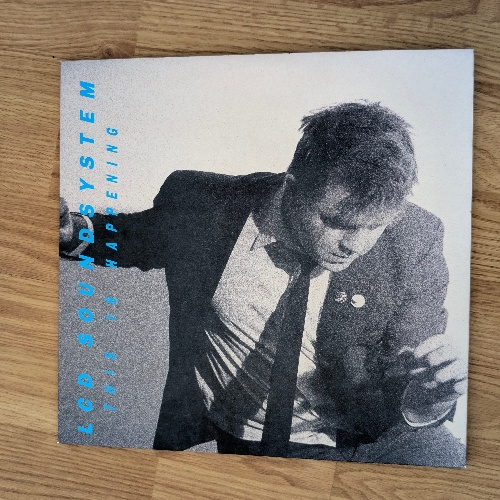
\includegraphics[width=0.45\textwidth]{figures/test_albums/This_Is_Happening_Rotated - 270.jpg}
        \caption{The only correct result for 270° rotation}
        \label{fig:tih_rotated_270}
    \end{subfigure}
\end{figure}

Despite the shortcomings of the reverse image search, the results indicate that the scatter-shot approach, using website titles, was equally or more successful across all categories of images. These results validate including it as it improves the overall chances of identification.

\begin{figure} [H]
    \centering
    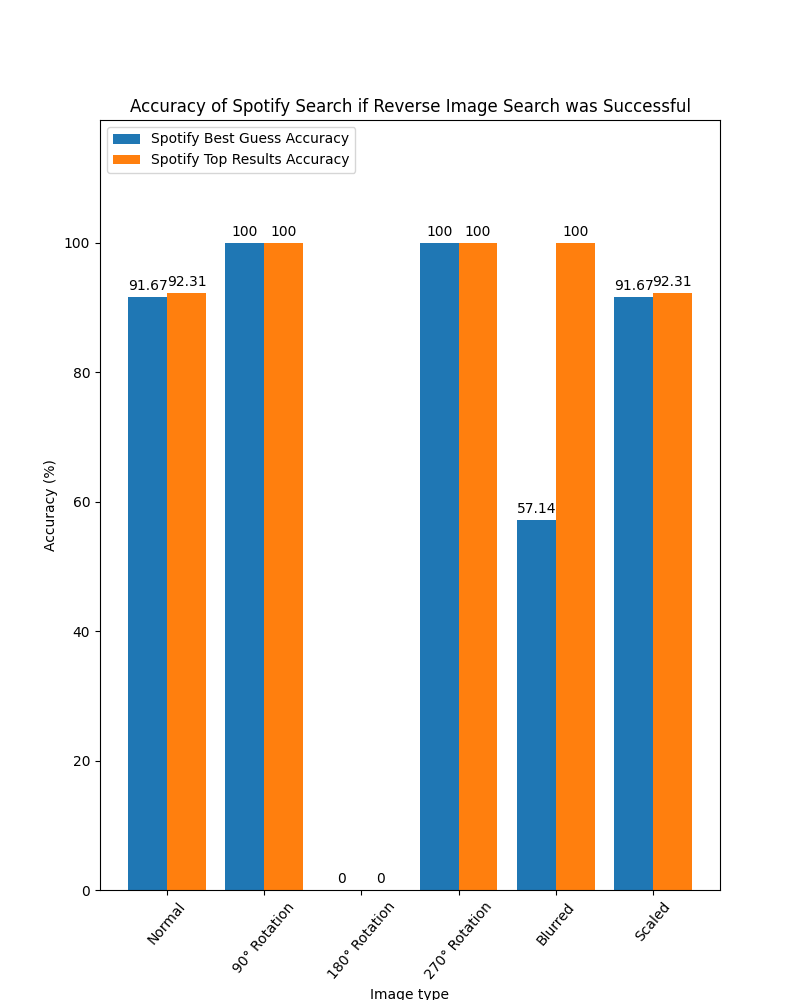
\includegraphics[width=0.65\textwidth]{figures/evaluation_graphs_spotify.png}
    \caption{Accuracy of Spotify Search}
    \label{fig:album-scanning-results-spotify}
\end{figure}

The results from the Spotify search API demonstrated strong performance. When provided with a correct reverse image search result, the Spotify search successfully identified the correct album in:

\begin{itemize}
    \item $91.67\%$ (11 out of 12 cases) for best guess searches.
    \item $92.31\%$ (12 out of 13 cases) for website title-based searches.
\end{itemize}

These results indicate that the chosen method, directly using reverse image search outputs with no processing as inputs for the Spotify search API, was broadly effective, even though it did not achieve the target $95\%$ accuracy.

\subsubsection{Key Takeaways}
The primary limiting factor in the system's accuracy is the reverse image search API's accuracy. Therefore, any changes hoping to improve the accuracy of album identification should focus on enhancing this API's accuracy.

Since the Google reverse image search API is treated as a black box, direct improvements to its internal processing are impossible, leaving only one option to improve its accuracy: input refinement. Two possible approaches include:

\begin{itemize}
    \item Pre-processing the image – Applying pre-processing techniques to remove backgrounds before passing the image to the API, for example, segmentation, where the image's background is removed automatically. %[TODO: Add a reference to segmentation potentially]
    \item User-assisted cropping – Prompting users to crop the image manually, ensuring only the album cover is submitted for identification
\end{itemize}

Though these methods may improve accuracy, the second could introduce additional UI elements, making the system more complex from a user perspective. The first may increase the time required to scan an album. Therefore, any enhancements should be carefully evaluated to balance accuracy improvements with user experience.

It should also be noted that the sample size for testing was relatively small, with only fifteen albums evaluated. As a result, the accuracy figures obtained may not fully represent the system's performance on a more extensive and diverse dataset. For example, less popular albums are likely less likely to be identified, and more popular albums are more likely to be identified. Testing with a broader selection of albums would be necessary to obtain a more comprehensive assessment of the system's accuracy and limitations.

\subsection{Album Playback}
This test aimed to verify that the music playback functionality operated as intended. The most effective approach was to evaluate the application from a user perspective, simulating real-world usage by using it to listen to whole albums, ensuring that playback functioned correctly.
\ifshowappendix
%Testing was conducted using a subset of five albums listed in Appendix~\ref{apd:test_albums}.
\fi

\subsubsection{Results}
The results of this test were entirely positive. All selected albums played from start to finish without issues. Additionally, the music controls, including play, pause, and skip—functioned as expected, and album artwork and track information were displayed correctly throughout playback as the tracks changed.

\section{User Interface}
The survey described in Section~\ref{sec:test-design} was used to evaluate the user interface. In total, seven participants completed the survey. Initially, the first user was given the application and asked to play around with it but based on their feedback the process was adjusted. Instead, users were given a list of objectives to complete to cover all functionality.

\subsection{Results}
\begin{table} [H]
    \centering
    \begin{tabular}{|m{5cm}|m{2cm}|m{2cm}|m{2cm}|}
        \hline
        \textbf{Question} & \textbf{Average} & \textbf{Minimum} & \textbf{Maximum} \\
        \hline
 How easy was the application to use? & $5.71$ & $3$ & $7$ \\
        \hline
 How visually appealing was the application? & $8.29$ & $6$ & $10$ \\
        \hline
 How useful did you find the ability to save albums to your collection? & $7.71$ & $5$ & $10$ \\
        \hline
 How valuable did/would you find the social features? & $5$ & $3$ & $8$ \\
        \hline
    \end{tabular}
    \caption{User Interface Evaluation Results}
    \label{tab:ui-evaluation-results}
\end{table}

The results for the first four questions in the survey are shown in Table~\ref{tab:ui-evaluation-results}.

\paragraph{Question 1: How easy was the application to use?}
In terms of usability, the application did not perform well. The average score was only $5.71$, suggesting most users struggled with the application at some point. This was most likely a result of the design of the interface. Some users added that certain features were hidden from them or not in the place they expected them to be. The example most frequently given was that the share collection buttons were not on the social page where they would make sense to be. One user also found they could not use the web browser of their choice as the application would appear broken. This was missed in testing as the developer only tested in Google Chrome.

\paragraph{Question 2: How visually appealing was the application?}
The visual appeal of the application was rated particularly highly, with an average score of $8.29$, though, as will be discussed in Section~\ref{sec:ui-evaluation-participants}, this could be a result of many participants sharing a view of what a visually appealing looks like.

\paragraph{Questions 3 and 4: How useful did you find the ability to save albums to your collection? \& How valuable did/would you find the social features?}
The two features that were asked about had very different perceptions from users. Having a collection associated with their account was seen as a good feature, with an average score of $7.71$. The social features were not seen as much of a benefit, with an average score of $5$. Users likely did not see the value in social features in such a small application.

\paragraph{Extra Comments From Users}
As part of the evaluation, users could add extra comments. Most were about UI design choices. Many users found the application different from what they would expect, and some struggled to figure out what to do on specific screens. This was particularly a problem on the landing screen, where users did not feel prompted to log in to continue.

Other users found minor visual bugs that were not picked up in testing. Variation in screen sizes was the most common cause of these bugs. During development, the developer focused on a single screen size and resolution (16:9 aspect ratio). This also limited the application's usability, with one user commenting that the application might be more useful on a phone.

\subsection{Participants}~\label{sec:ui-evaluation-participants}
Ideally, the user interface evaluation would have been conducted with a large and diverse user base to gather feedback from individuals with varying levels of technical expertise. However, this was beyond the scope of the current evaluation, so a smaller sample group was used instead.

It is important to acknowledge the potential biases in the participant selection. The sample group consisted primarily of friends and family, many of whom were computer science students. As a result, the participants may have been more familiar with the technology than the average user. They could also have been predisposed to providing more favourable reviews as to not disappoint the application's developer. Because of this, while the survey provides valuable insights, the findings may not fully represent a broader user base.

\section{Development Practices}
The development practices were evaluated based on the tests in Section~\ref{sec:test-design}. A pass was defined as meeting the verification specified.

\subsection{Testing And Test Coverage}
All tests defined in all test cases were executed and passed, as expected, as automated actions enforced this before code could be merged into the main branch of the repository.

Test coverage was measured using pytest-cov for the backend and Vitest for the frontend. The target was set at $95\%$ line and branch coverage for both the frontend and backend. The results are shown in Table~\ref{tab:test-coverage-results}.
\begin{table} [H]
    \centering
    \begin{tabular}{|m{3cm}|m{3cm}|}
        \hline
        \textbf{Component} & \textbf{Coverage} \\
        \hline
        Backend & $100\%$ \\
        \hline
        Frontend & $95\%$ \\
        \hline
    \end{tabular}
    \caption{Test Coverage Results}
    \label{tab:test-coverage-results}
\end{table}

The backend achieved full coverage with all lines and branches tested. The frontend achieved $95\%$ coverage, which whilst meeting the target, the fact it was below $100\%$ is likely a result of the inexperience of the developer in frontend development with many changes needed even after the tests were originally defined.

However, as was seen in the user evaluation of the interface, the tests did not manage to catch all minor issues suggesting the automated tests were either not comprehensive enough or secondary measures needed to be taken to ensure the application was fully functional.

In terms of the initial criteria set out in Section~\ref{sec:test-design}, the result was a success. But in terms of producing a fully functional, bug free application, the tests alone were not enough suggesting the initial criteria were not stringent enough.

\ifshowappendix
%A complete list of the tests can be found in Appendix~\ref{apd:testcases}.
\fi

\subsection{Code Quality}
Using pre-commit hooks successfully achieved the code quality objectives of enforcing formatting and linting. This ensured that all code committed to the repository adhered to established formatting and linting rules.

Though this approach was practical for a single developer, in hindsight, it may not have been ideal for team-based development because pre-commit hooks require each developer to install them manually. A much more robust approach would have been to enforce these rules using GitHub Actions that run on pull requests. This could either format the code itself or reject the pull request if the code did not meet the required standards, forcing the developer to run the formatting and linting tools locally before pushing their changes, achieving the same goal as the pre-commit hooks.

\subsection{Automated Deployment and Dependency Management}
The automated deployment process was successfully implemented. Once configured on Google Cloud Run, the application could be rebuilt and deployed automatically whenever a new tag was pushed to the repository.

Similarly, automated dependency management was effectively set up using Dependabot, with weekly checks for updates. Throughout development, $110$ pull requests were generated for dependency updates, with only three requiring manual intervention, primarily due to breaking changes. It is of note that none of the changes that passed all tests resulted in breaking changes to the application, suggesting that the testing system in place was effective in verifying functionality after each update.

\chapter{Conclusions}~\label{cha:conclusion}

\section{Conclusions}
This project focused on developing and deploying a web application that functions like a traditional turntable. In this sense, it should be considered a success, as in most cases, it succeeds based on the criteria set out that it should use a representation of the physical album as input to play the whole album. However, the system's inaccuracy in identifying albums could be considered a failure, especially considering it is the only way to listen to music using the application.

In terms of planning, the project closely followed what was set out in Section~\ref{sec:plan}, and the agile methodology proved to be a good fit for the project. The Kanban board was a good way to manage tasks and was effective when issues arose that had to be added to the board. The architectural decisions in the design phase proved well-thought-out as no issues arose during development that required a rethink of the architecture. The backend structure needed no changes to the initial design other than the change to a different DBMS, which was quickly done due to the choice of SQLAlchemy as an ORM. The frontend, though having some issues, was technically well implemented and the design included all features.

The intention to keep to good software development practices proved very successful. Automated test coverage gave high confidence that the application was working as intended, with the only exception being minor visual bugs on the frontend. In conjunction with automated dependency management, the project could always use the latest versions of dependencies, ensuring no known vulnerabilities existed. The automated deployment also proved successful, with the application automatically being built and deployed on the cloud whenever a commit was tagged on the repository's main branch.

The evaluation of the project showed that the application was well received by users but also showed the flaws in the application. The UI was not perfect, and some features could have been added. The social features were not used by many users, suggesting a rethink of these features could benefit the application greatly.

\section{Future Work}
The evaluation revealed that the application was not perfect. In terms of improvements to the currently implemented features, future work should focus on improvements to the album identification system, given that it did not perform as well as hoped. The only option for improving the current system would be adding refinement techniques to the input image, hopefully improving the reverse image search API results. An alternative would be to implement new methods alongside the current one, such as OCR or barcode scanning. The user could then switch between methods if the current one fails, improving the chances that the scan will be successful.
Alternatives could also ditch the `scanning' concept entirely and use different methods. An example was given by a participant in the evaluation of using audio fingerprinting to identify albums from their audio~\cite{Cano2005}. An ultimate fail-safe could be to allow the user to search for the album manually.

On a larger scale, the application could be ported to mobile devices as an app. This development would require either a new frontend or a major rework of the current one to work on smaller screens with different aspect ratios from desktop screens.


\bibliography{refs}    % this causes the references to be listed

\bibliographystyle{abbrv}
%% the bibliography style determines the format  in which both citations and references are printed,
%% other possible values are plain and abbrv
%%
%% If you want more control of the format of your citations you might want to take a look at
%% natbib.sty, which should be part of any standard LaTeX installation
%%
%% University regulations simply require that your citation style be consistent, so see what style
%% your supervisor recommends.

\ifshowappendix
% Appendices start here

\appendix
%\chapter{Appendix 1: Testcases} \label{apd:testcases}

\section{Frontend Testcases} \label{sec:frontend_testcases}

\section{Backend Testcases} \label{sec:backend_testcases}

%\chapter{Appendix 2: Frontend components} \label{apd:frontend-components}

%\chapter{Appendix 3: Backend endpoints} \label{apd:backend-endpoints}

\chapter{Appendix 1: Test Albums} \label{apd:test_albums}
% List all images in a big tables
\begin{table}[h]
    \centering
    \renewcommand{\arraystretch}{1.5} % Adjust row height
    \setlength{\tabcolsep}{10pt}      % Adjust column spacing
    \begin{tabular}{|m{4cm}|m{4cm}|m{4cm}|} % Adjust column widths as needed
        \hline
        \textbf{Album Name} & \textbf{Artist} & \textbf{Cover} \\
        \hline
        Animals & Pink Floyd & 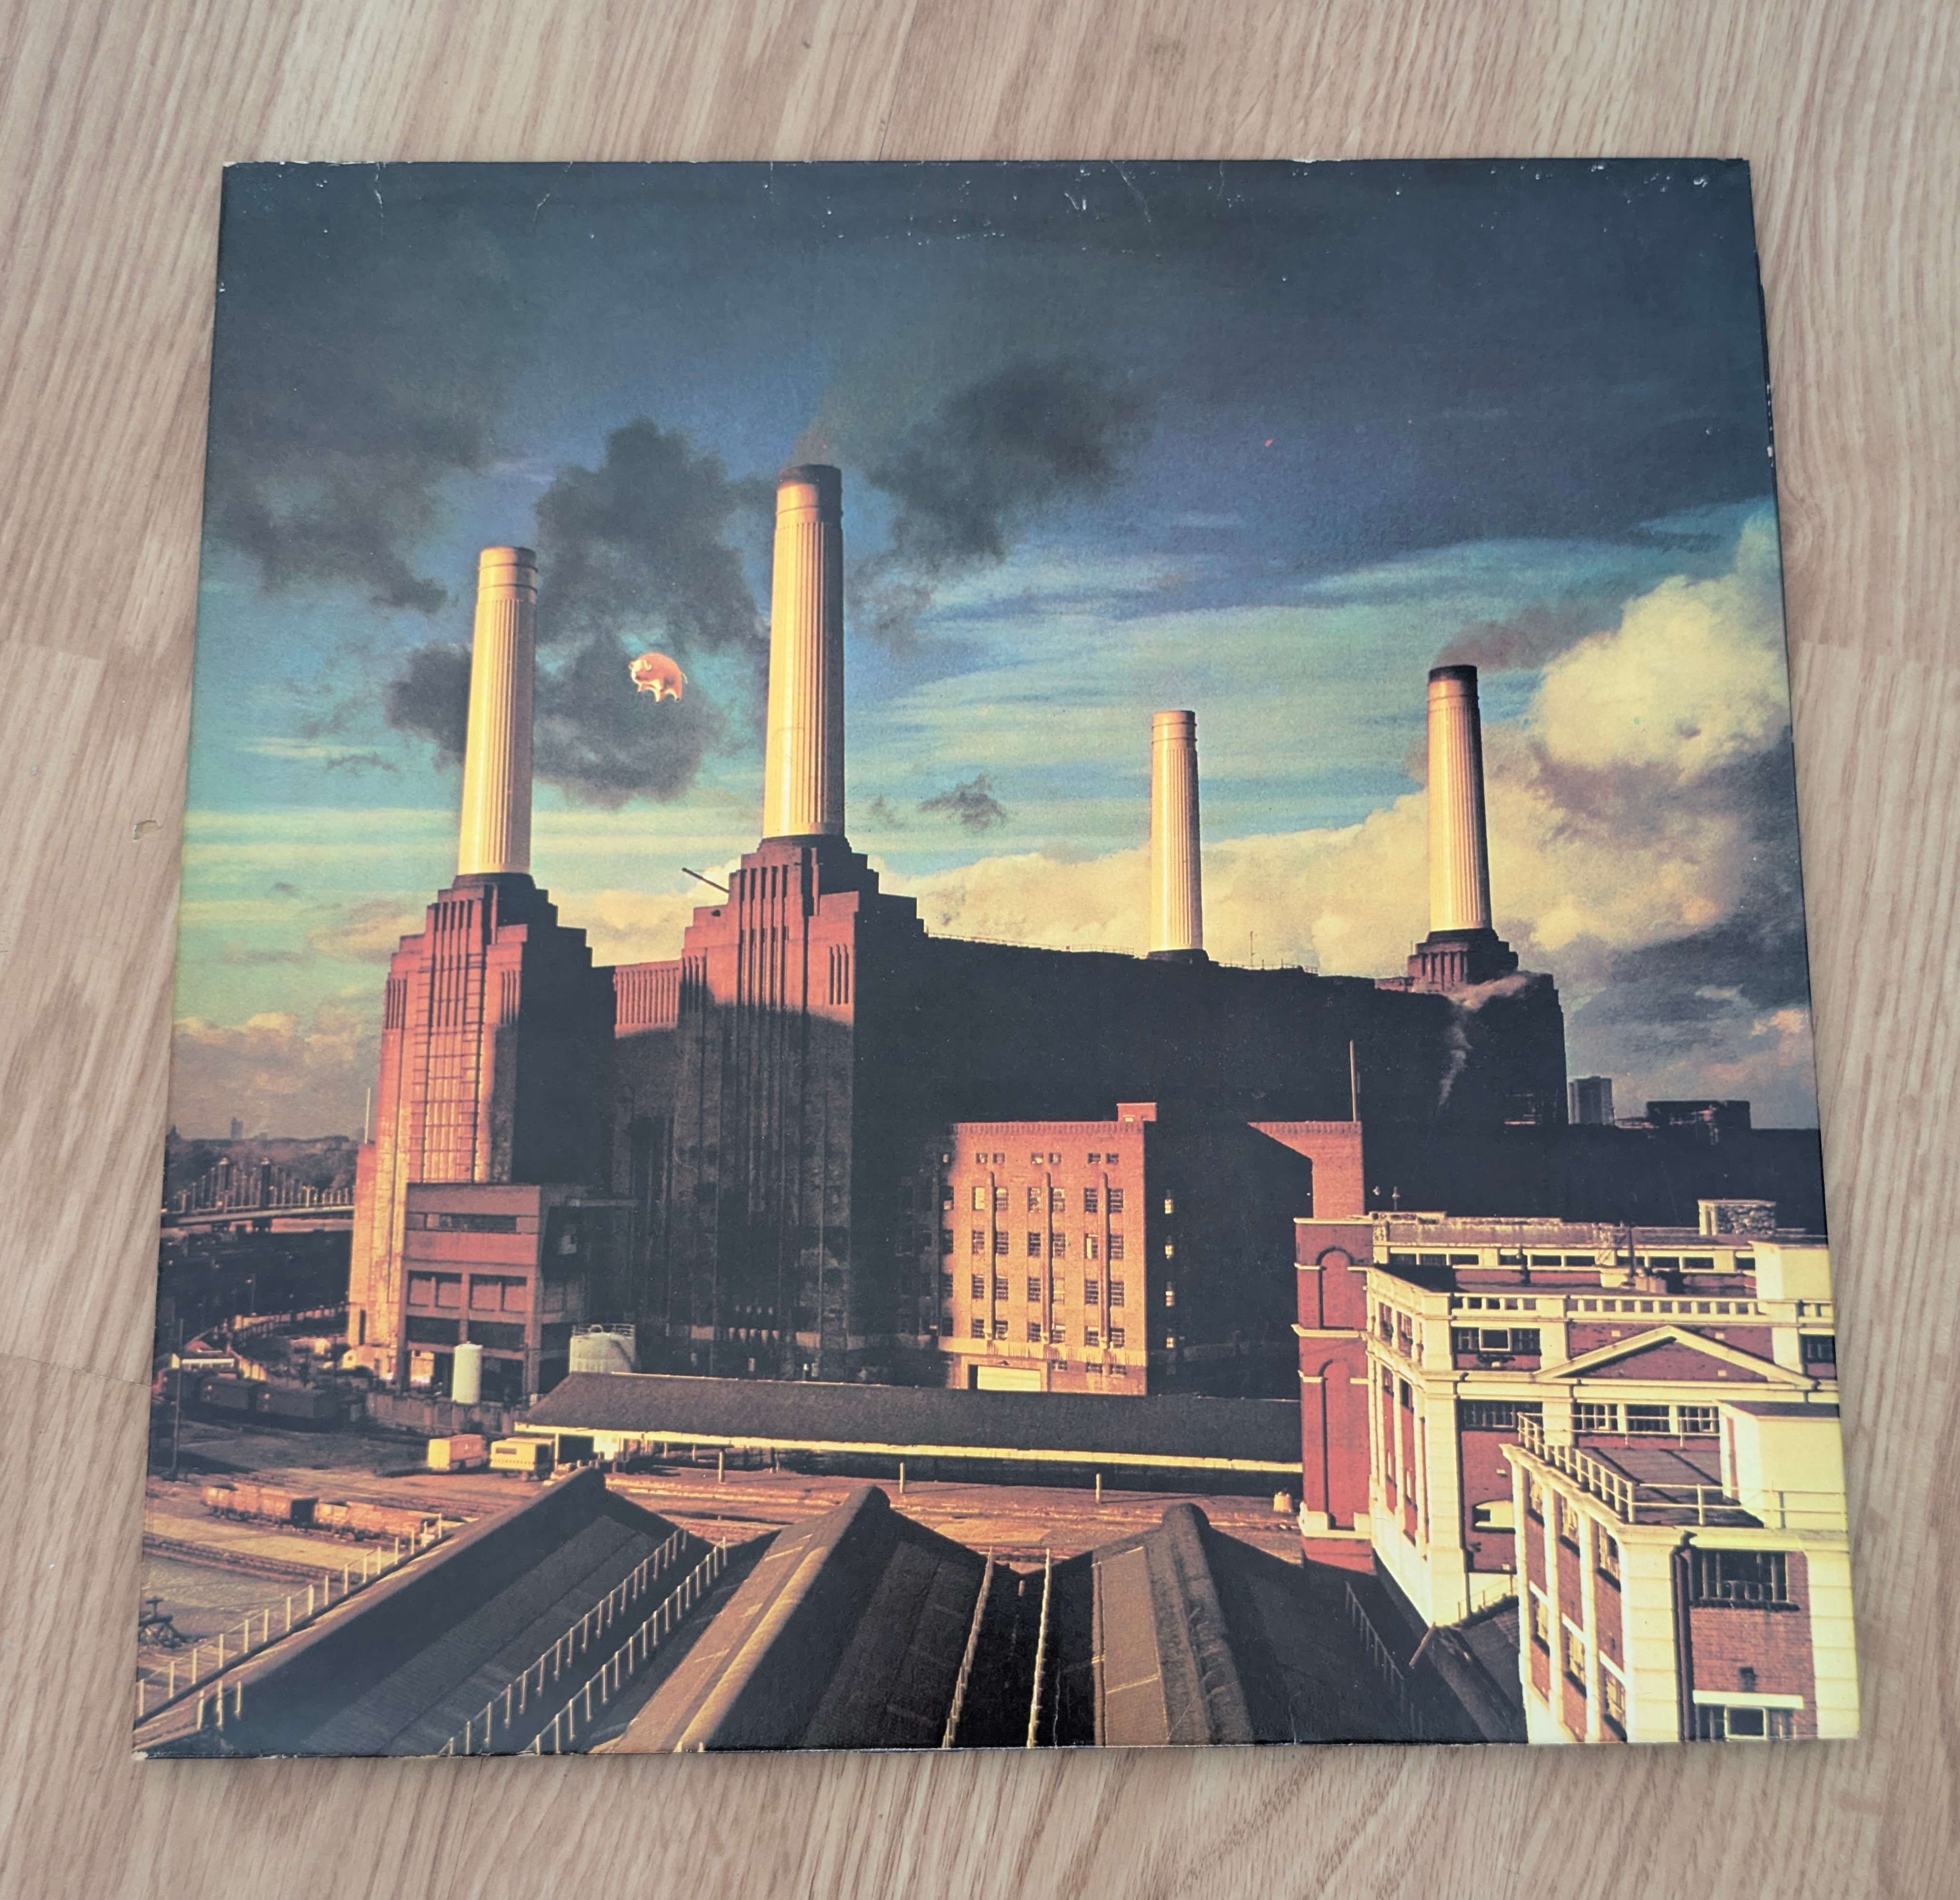
\includegraphics[width=2.5cm]{figures/test_albums/Animals.jpg} \\
        \hline
        Beatles 1962 - 1966 & The Beatles & 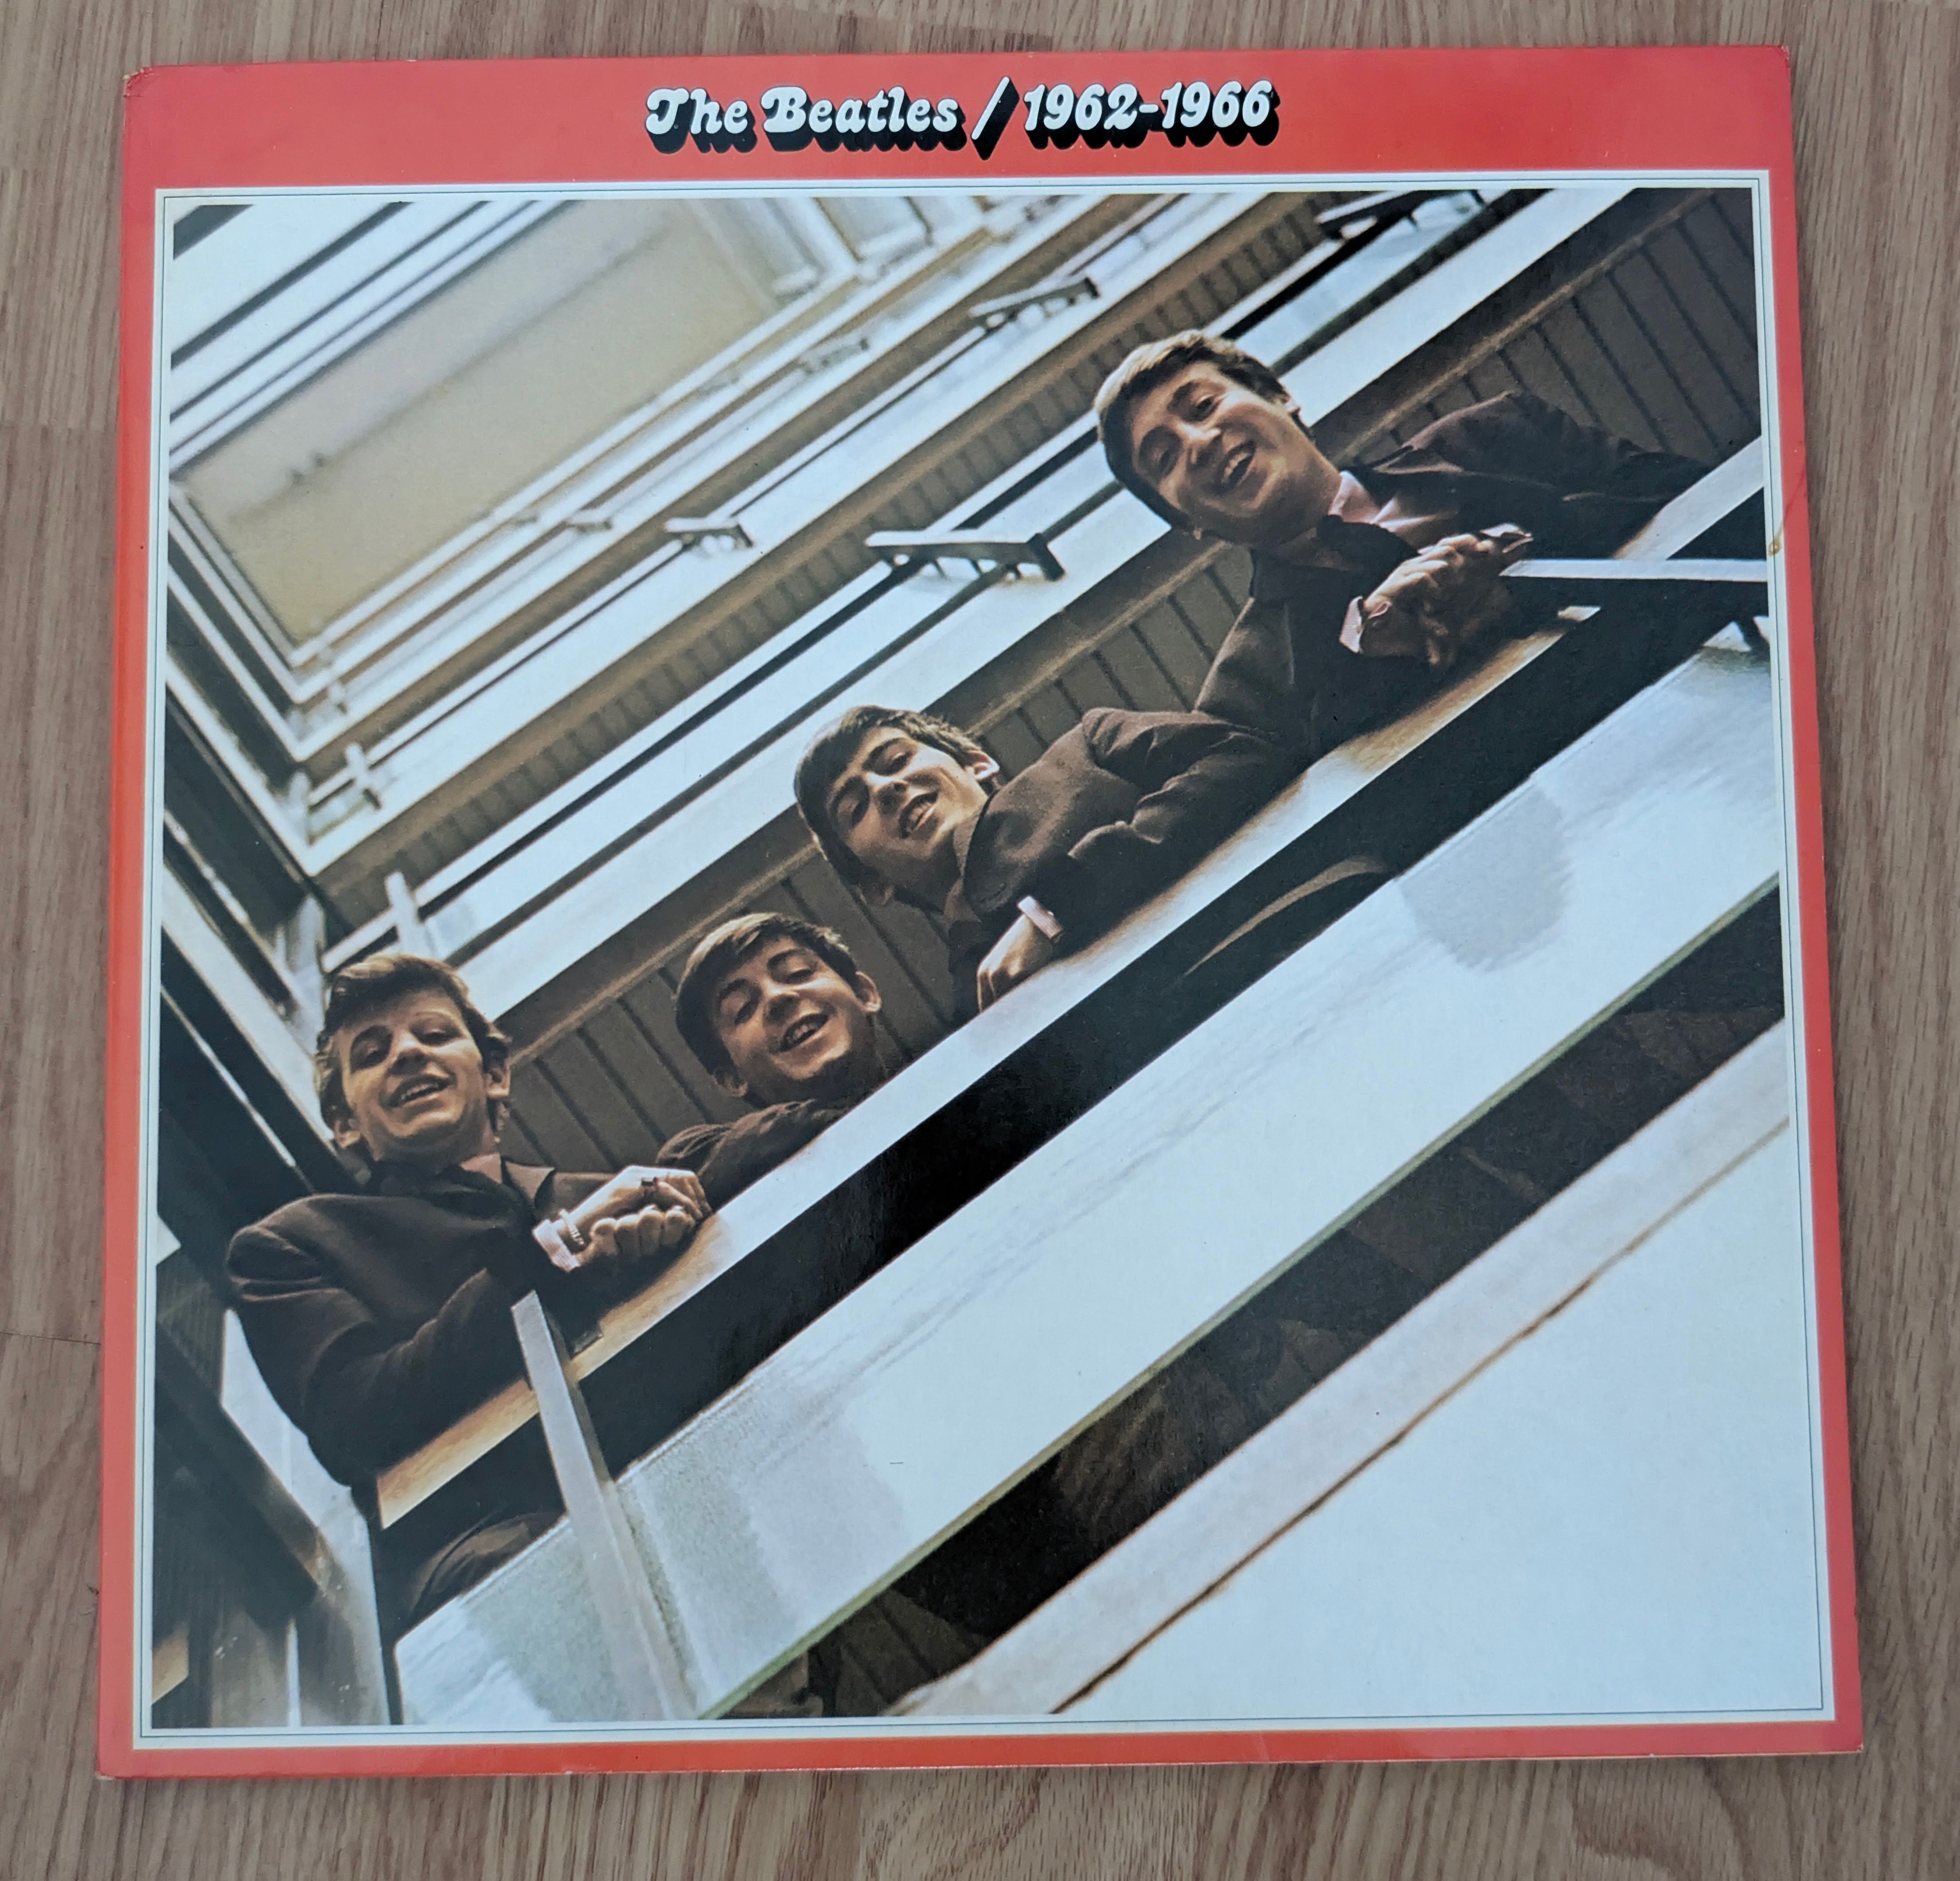
\includegraphics[width=2.5cm]{figures/test_albums/Beatles 62-66.jpg} \\
        \hline
        Beatles 1967 - 1970 & The Beatles & 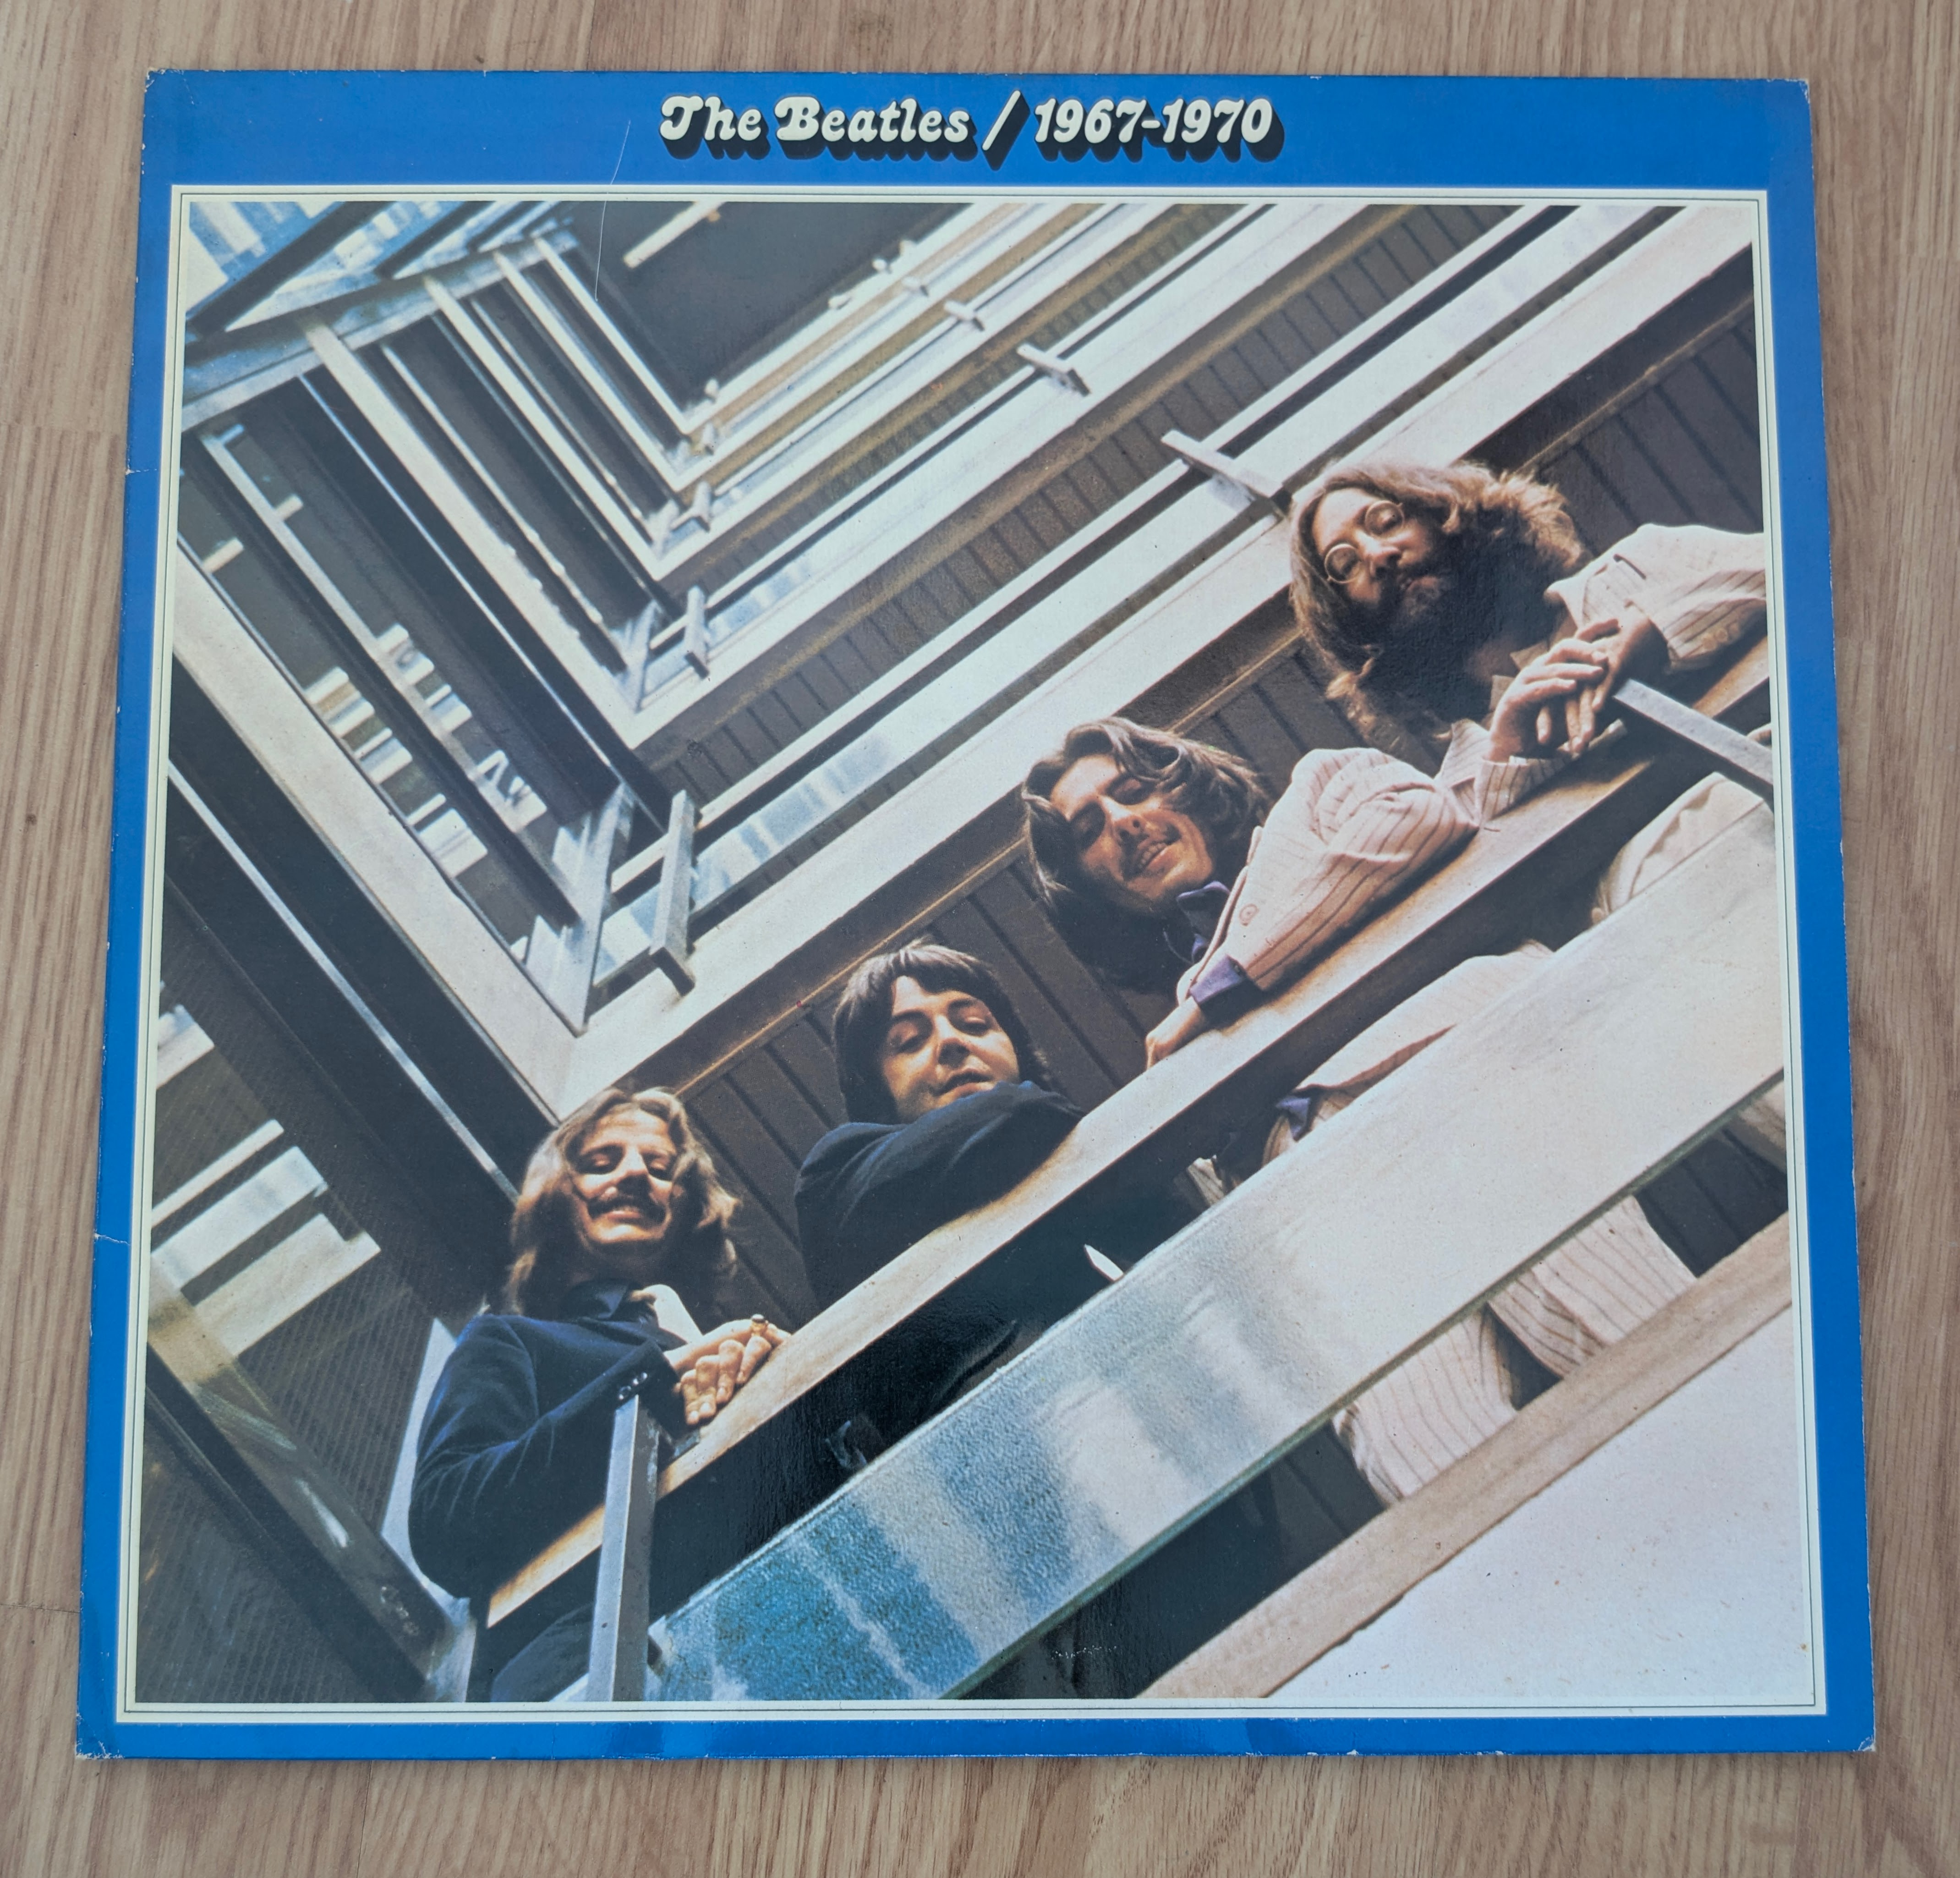
\includegraphics[width=2.5cm]{figures/test_albums/Beatles 67-70.jpg} \\
        \hline
        Being Funny In A Foreign Language & The 1975 & 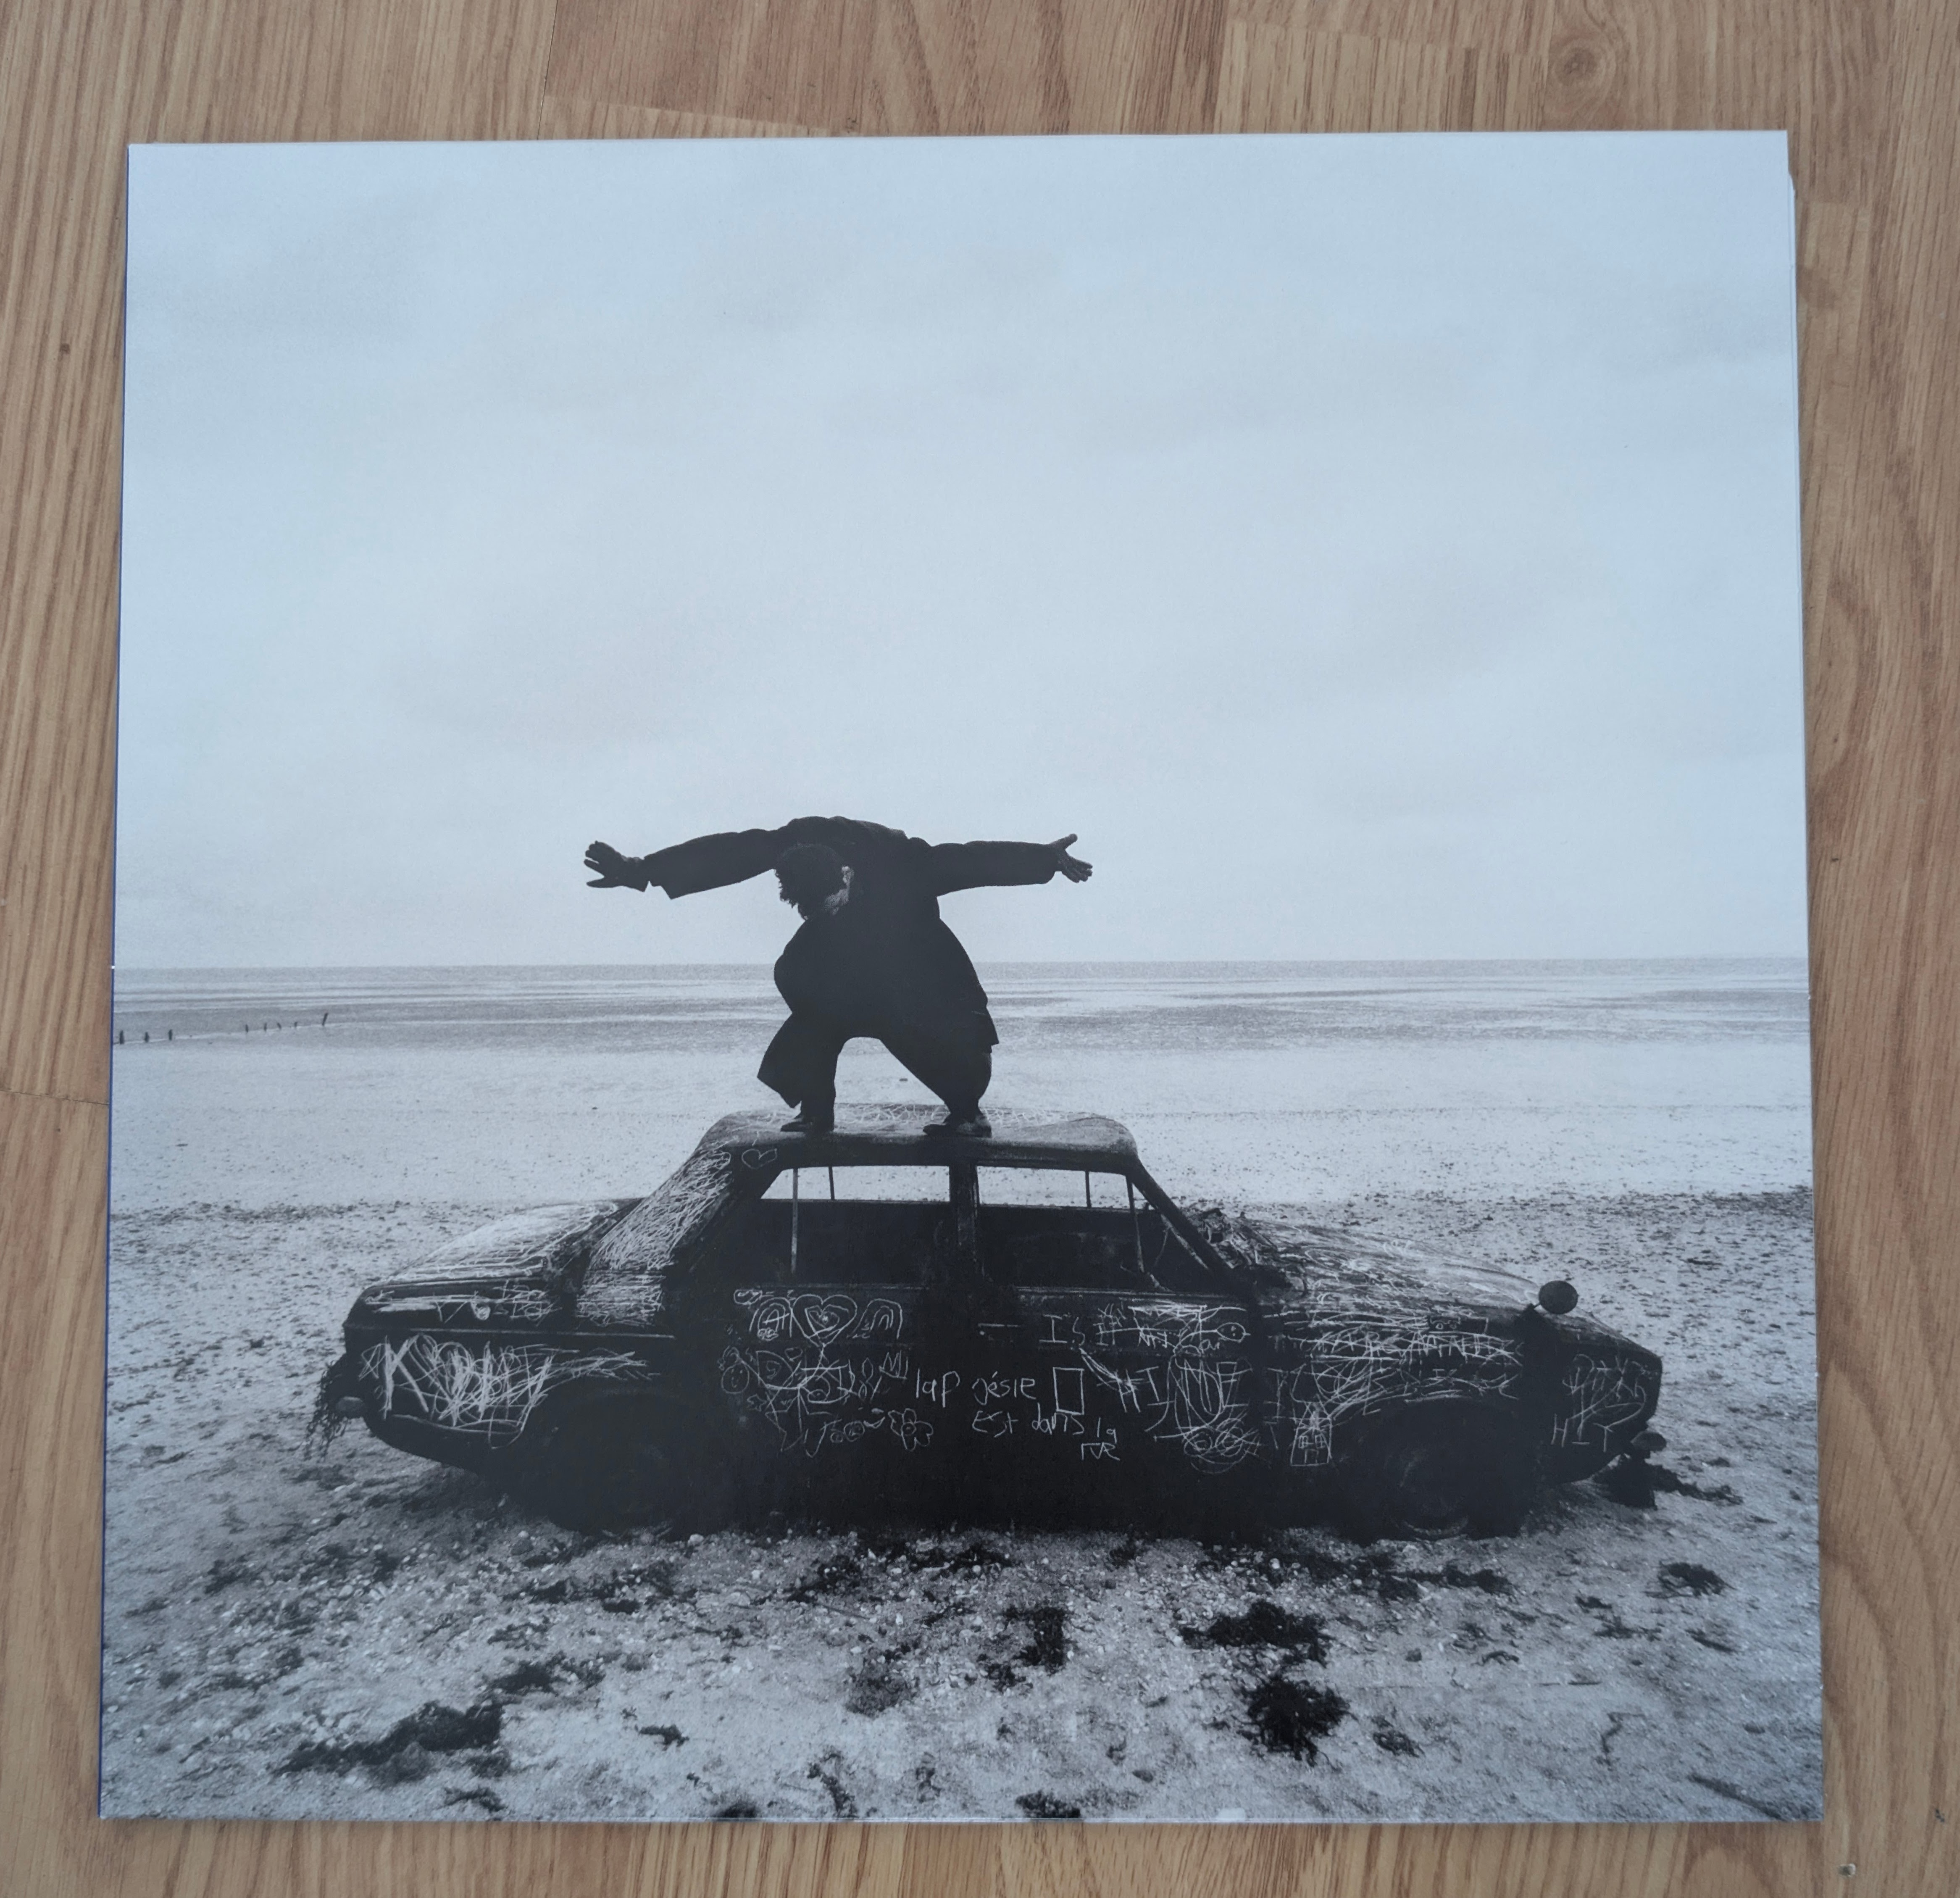
\includegraphics[width=2.5cm]{figures/test_albums/Being Funny In A Foreign Language.jpg} \\
        \hline
    \end{tabular}
    \caption{Album List with Cover Images}
    \label{tab:albums-list1}
\end{table}

\begin{table}[h]
    \centering
    \renewcommand{\arraystretch}{1.5} % Adjust row height
    \setlength{\tabcolsep}{10pt}      % Adjust column spacing
    \begin{tabular}{|m{4cm}|m{4cm}|m{4cm}|} % Adjust column widths as needed
        \hline
        \textbf{Album Name} & \textbf{Artist} & \textbf{Cover} \\
        \hline
        Different Class & Pulp & 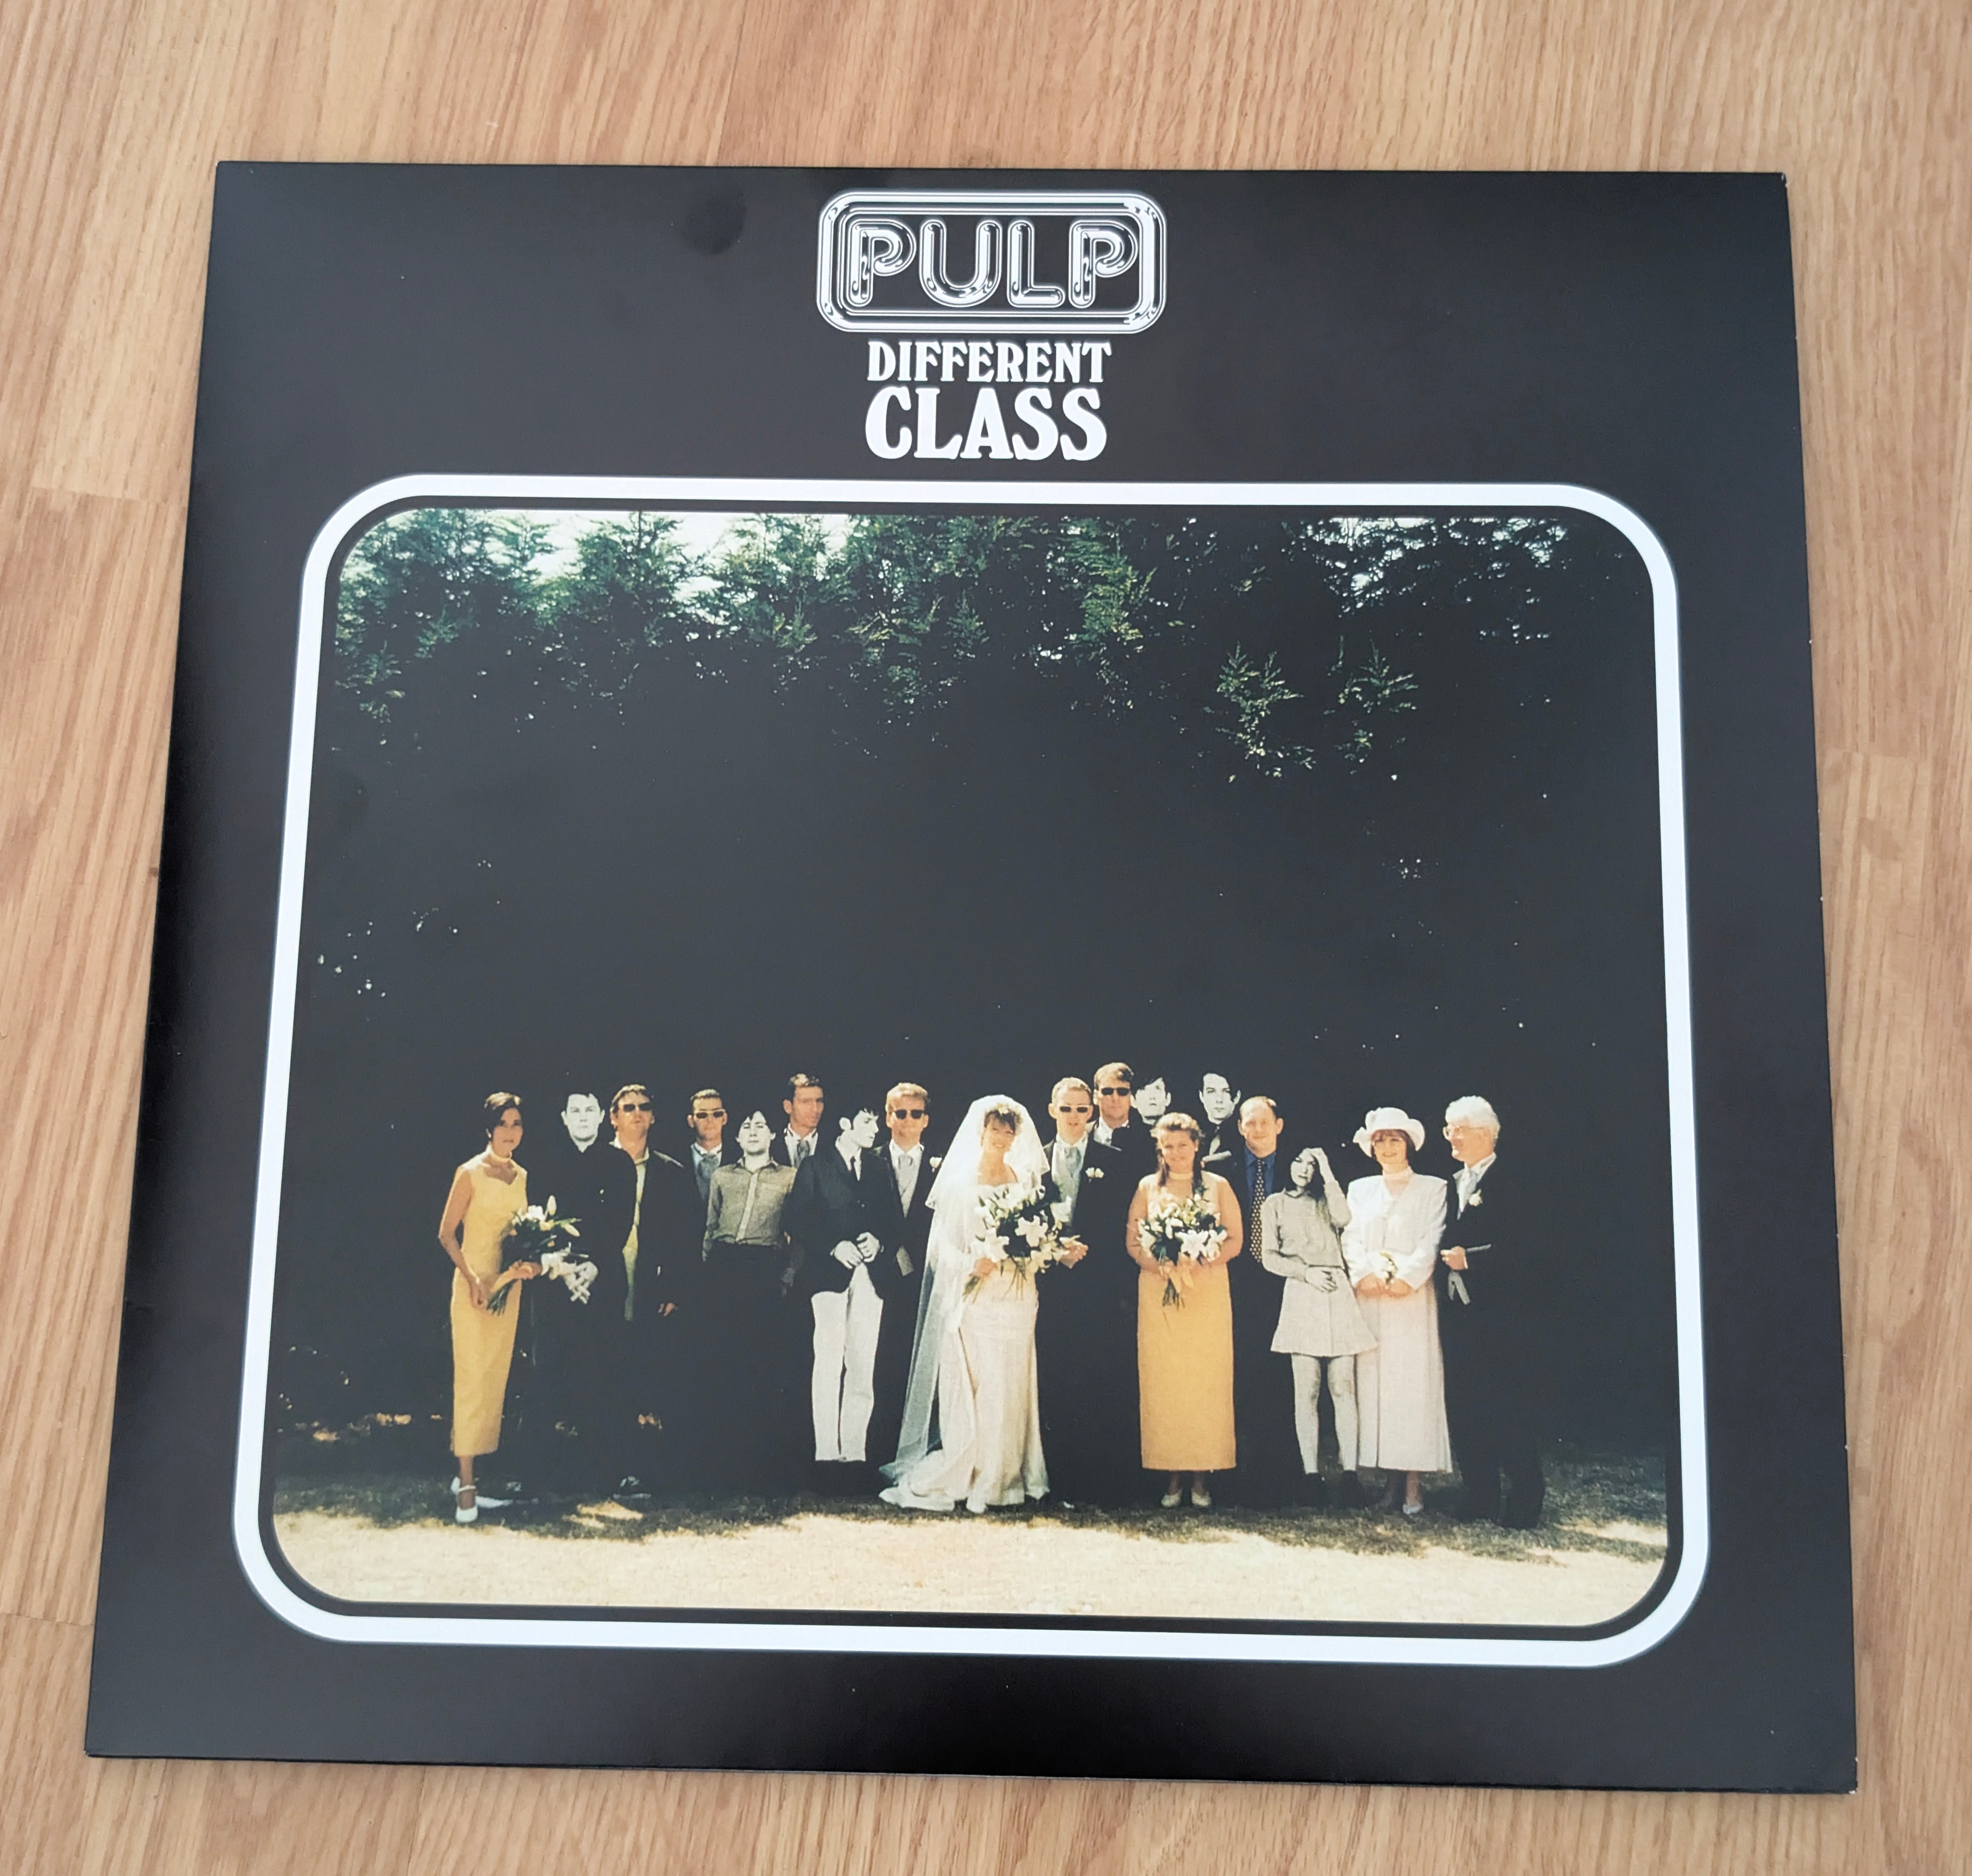
\includegraphics[width=2.5cm]{figures/test_albums/Different Class.jpg} \\
        \hline
        Fix Yourself Not The World & The Wombats & 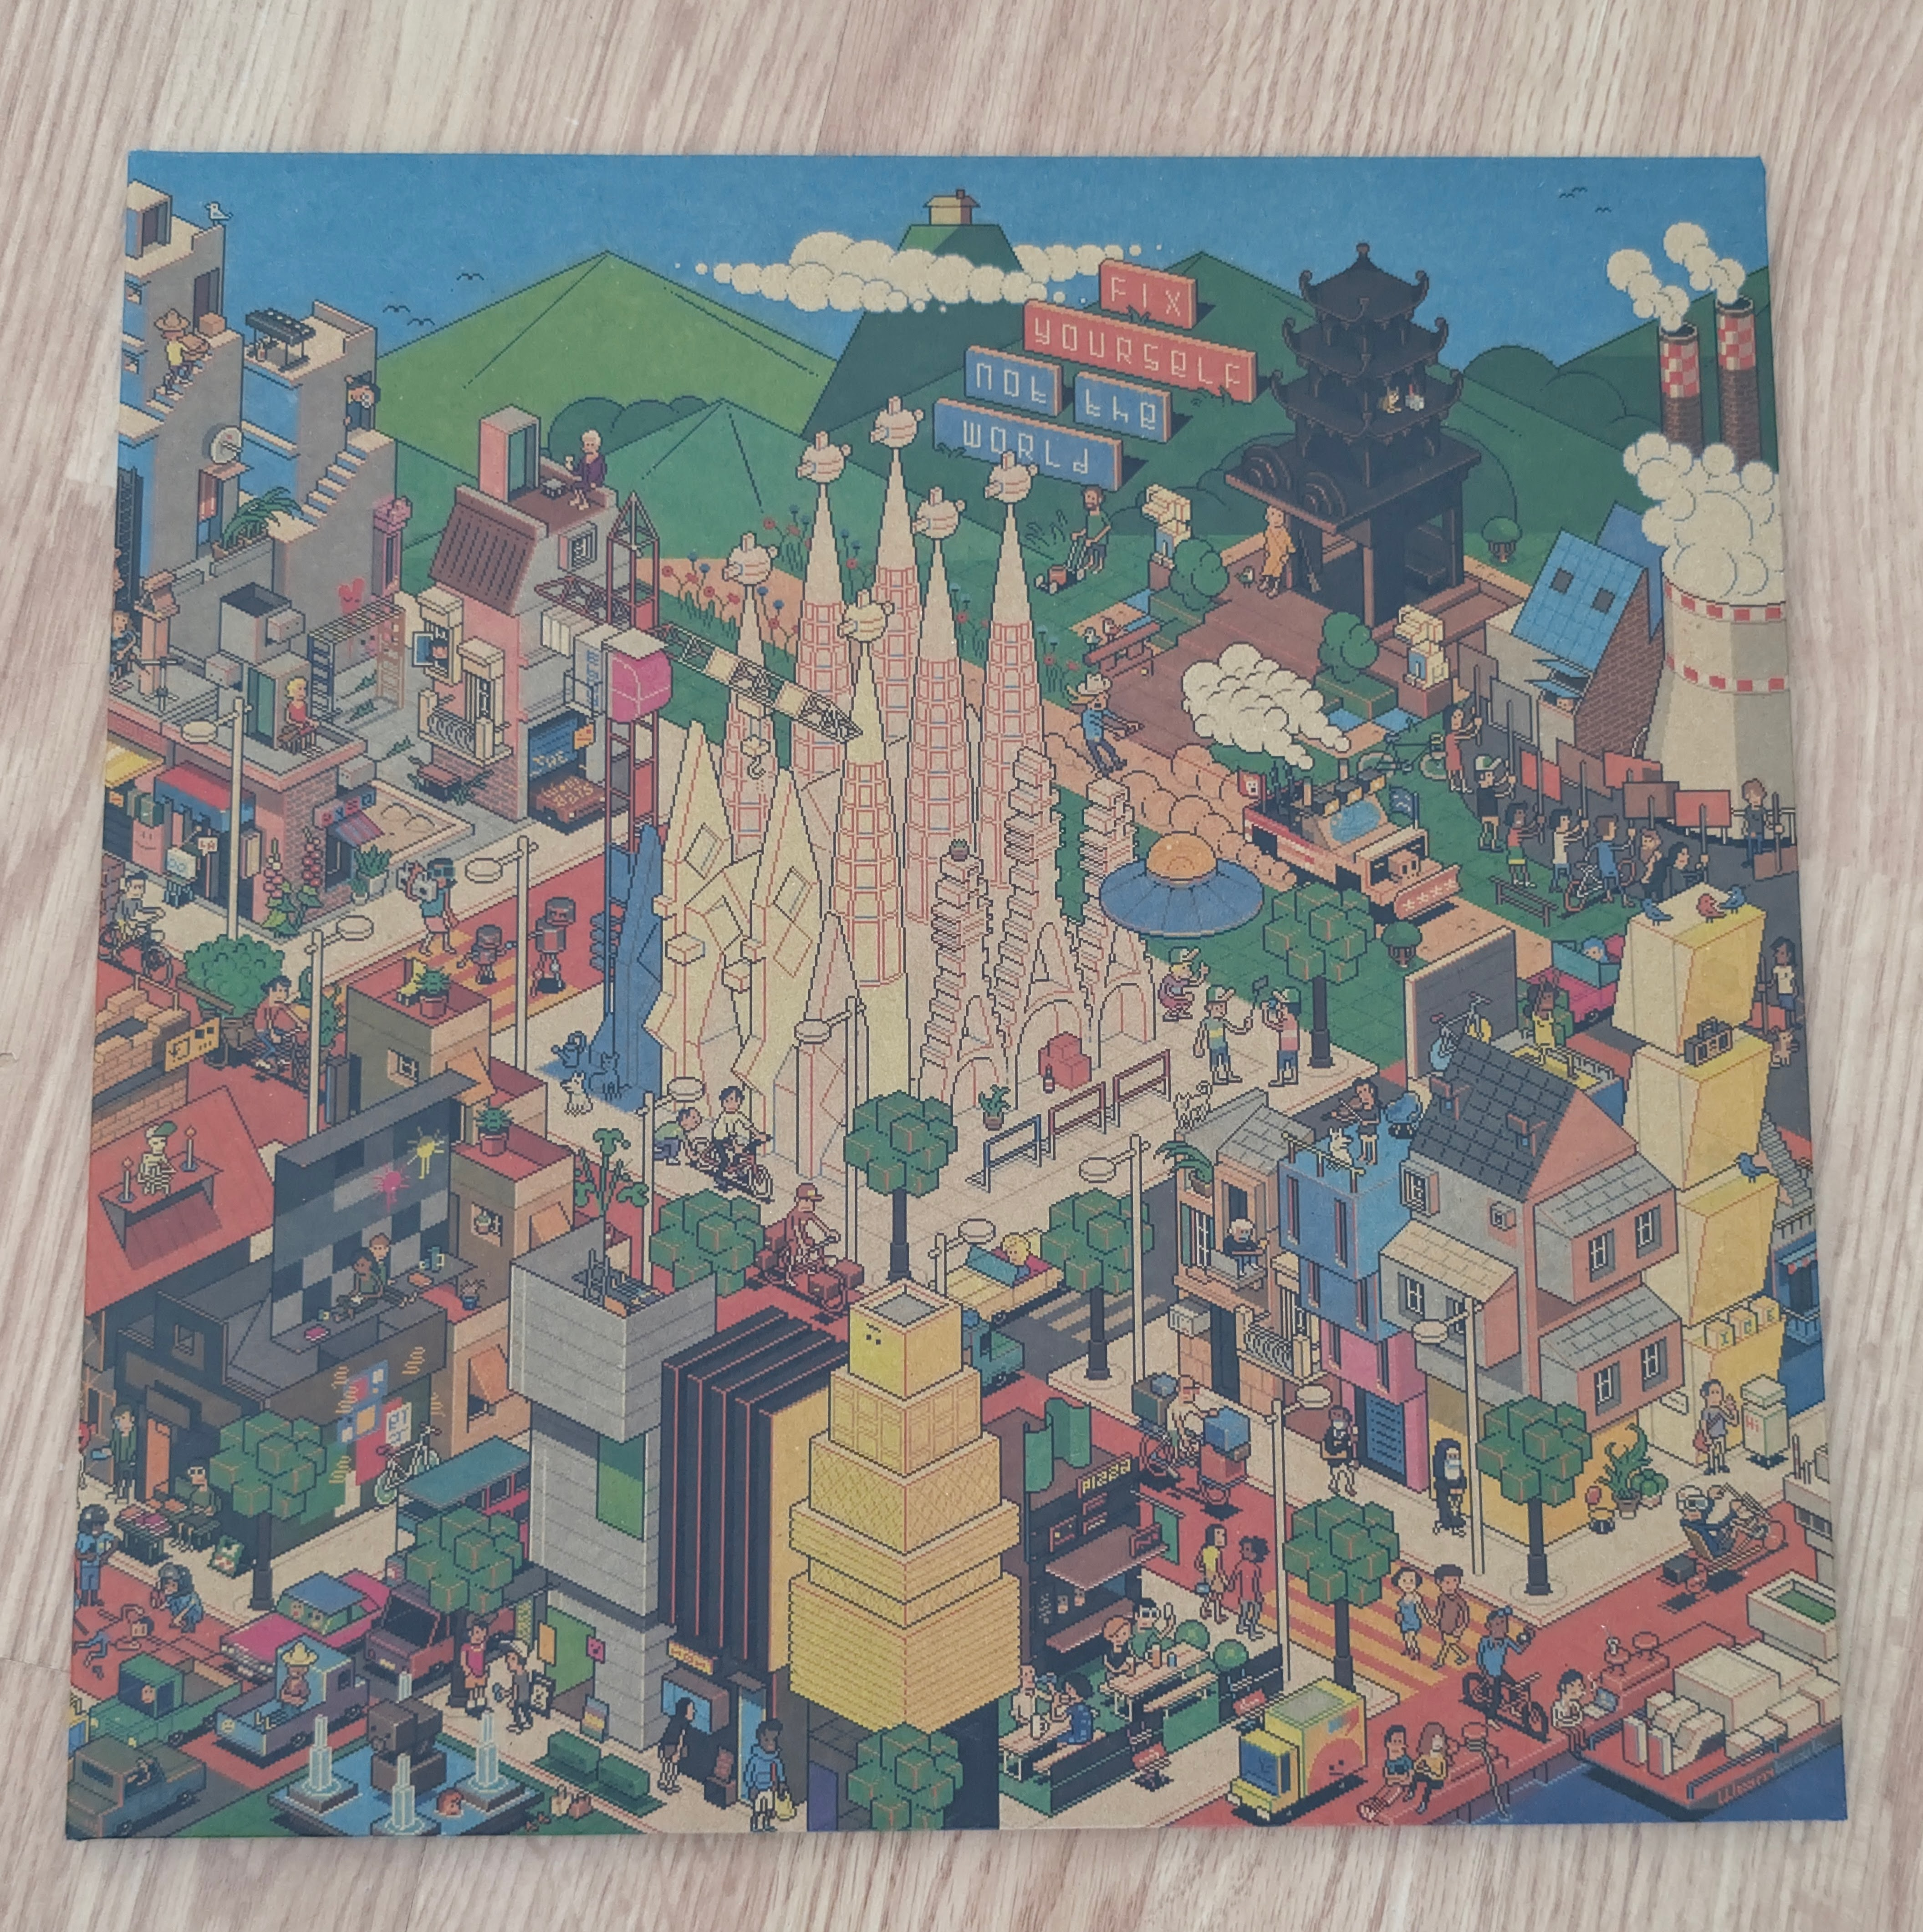
\includegraphics[width=2.5cm]{figures/test_albums/Fix yourself not the world.jpg} \\
        \hline
        Funeral & Arcade Fire & 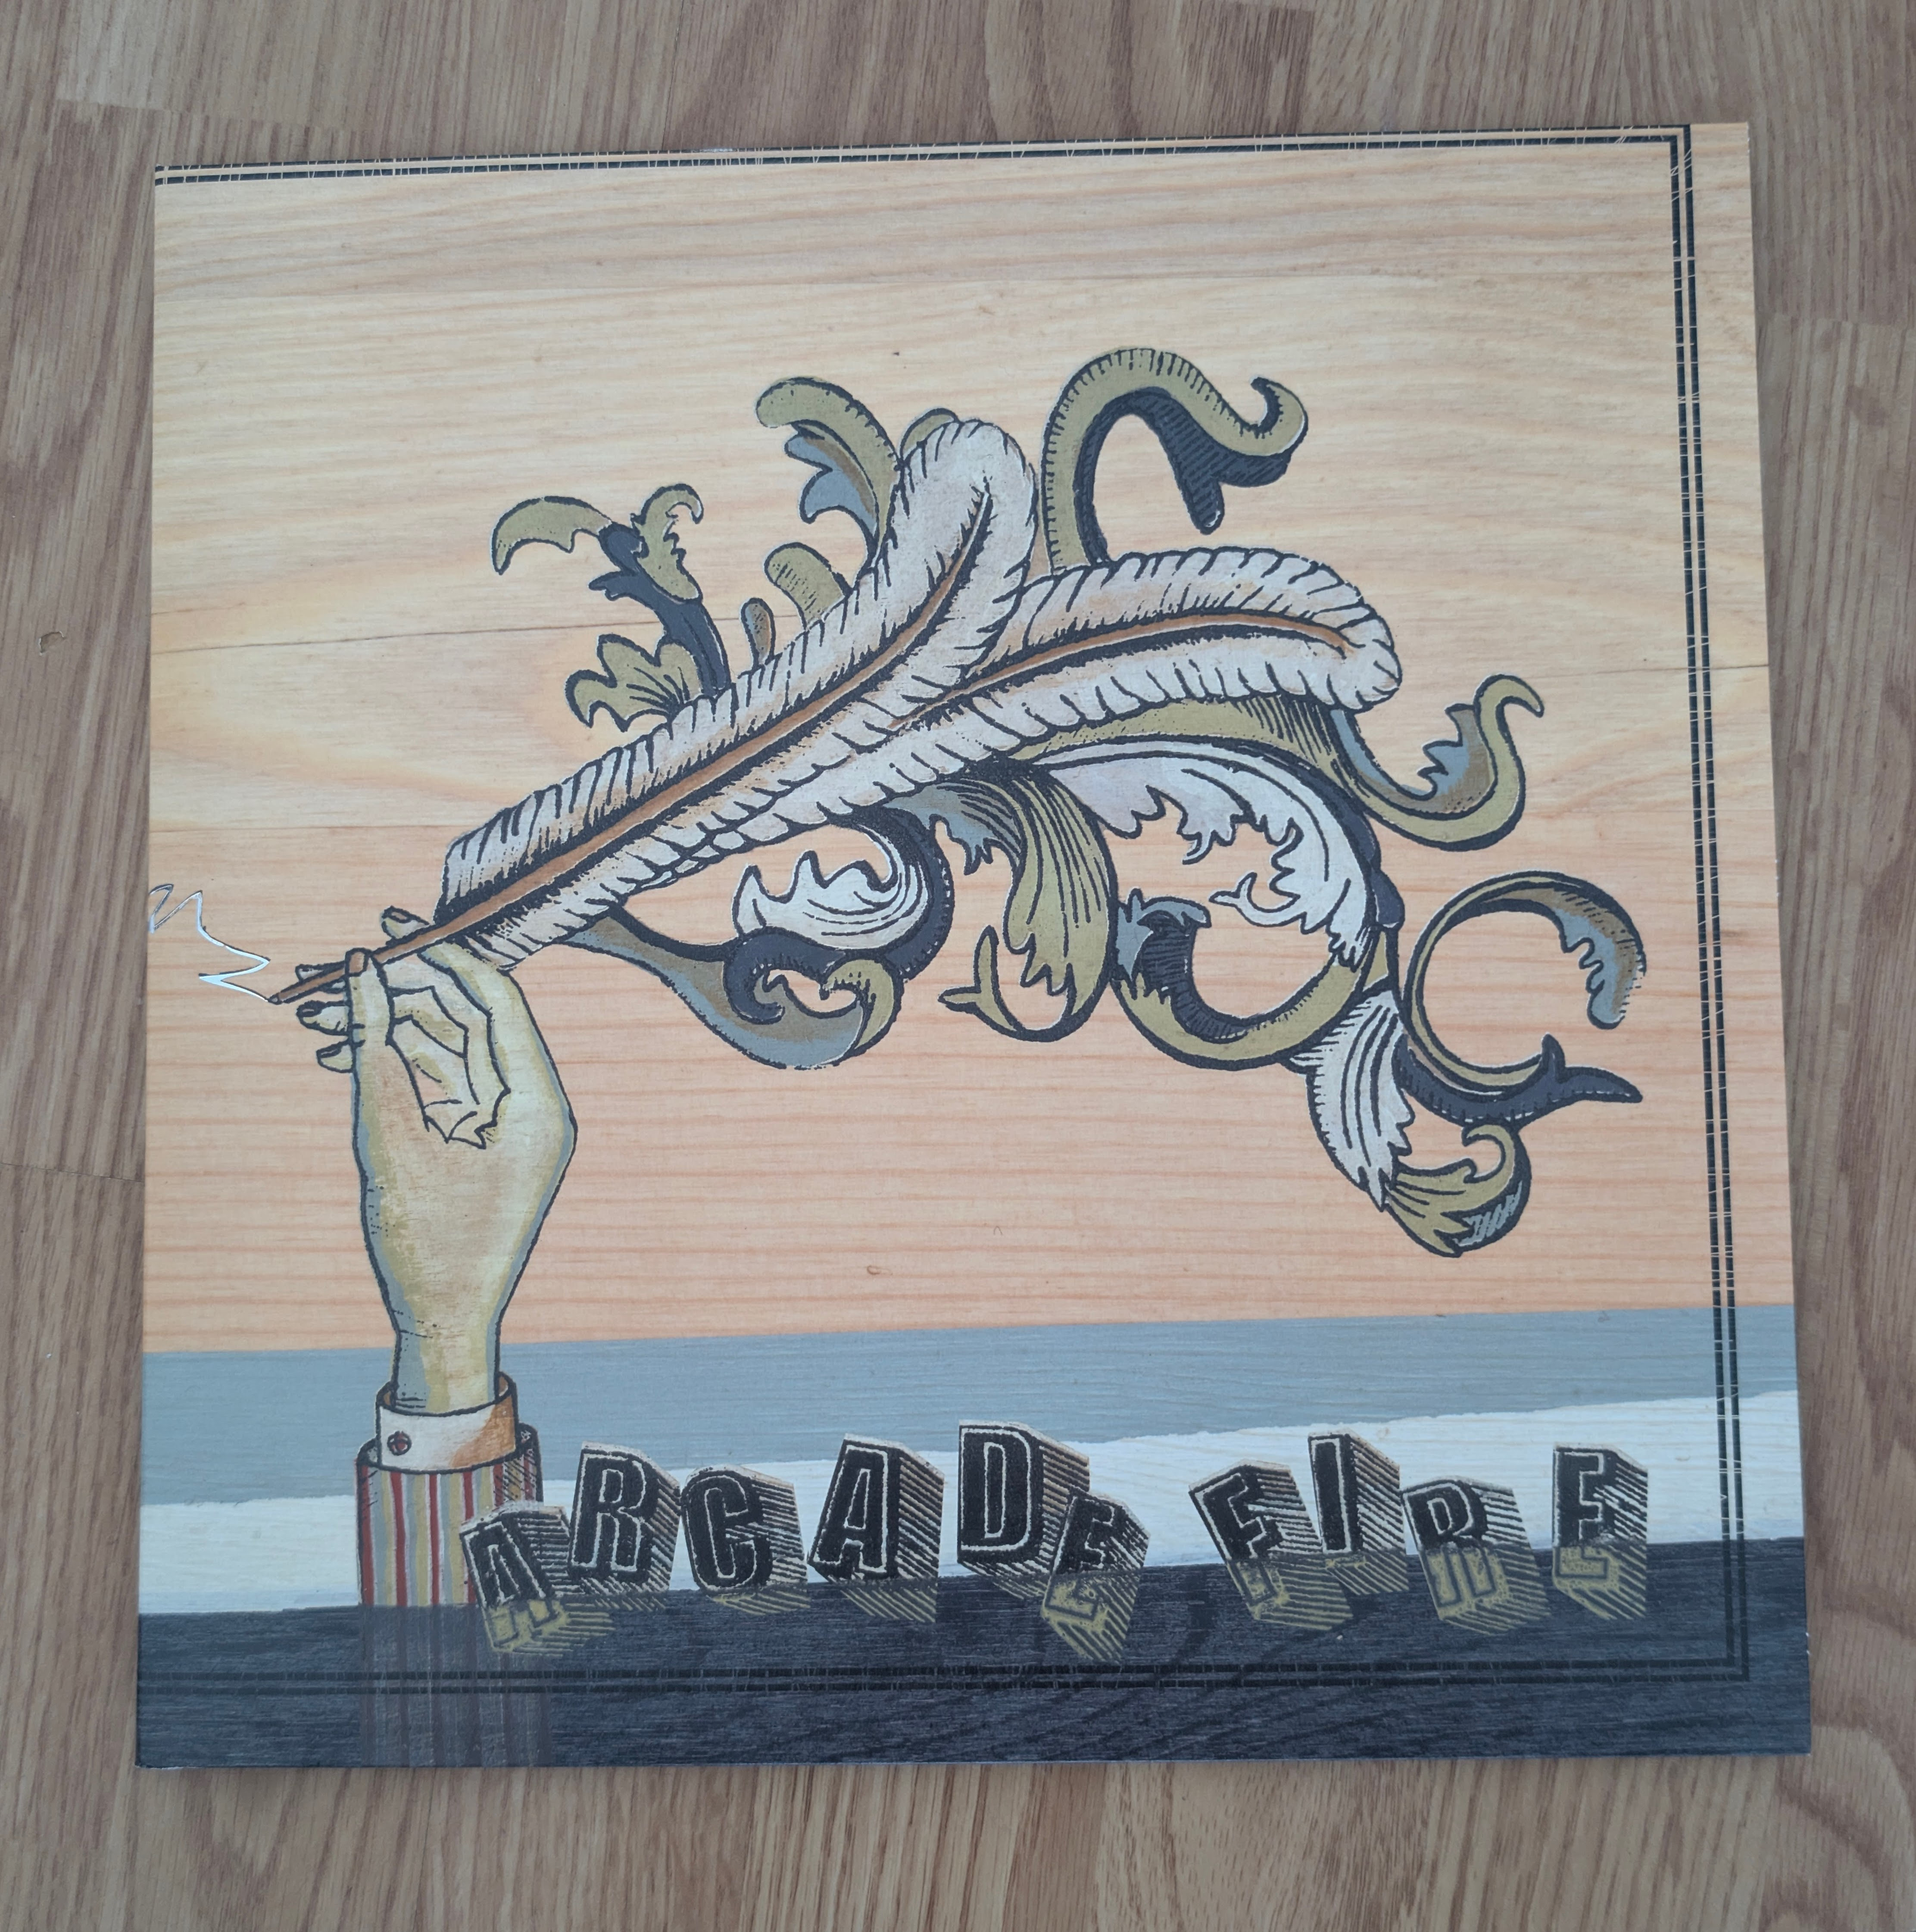
\includegraphics[width=2.5cm]{figures/test_albums/Funeral.jpg} \\
        \hline
        Glitterbug & The Wombats & 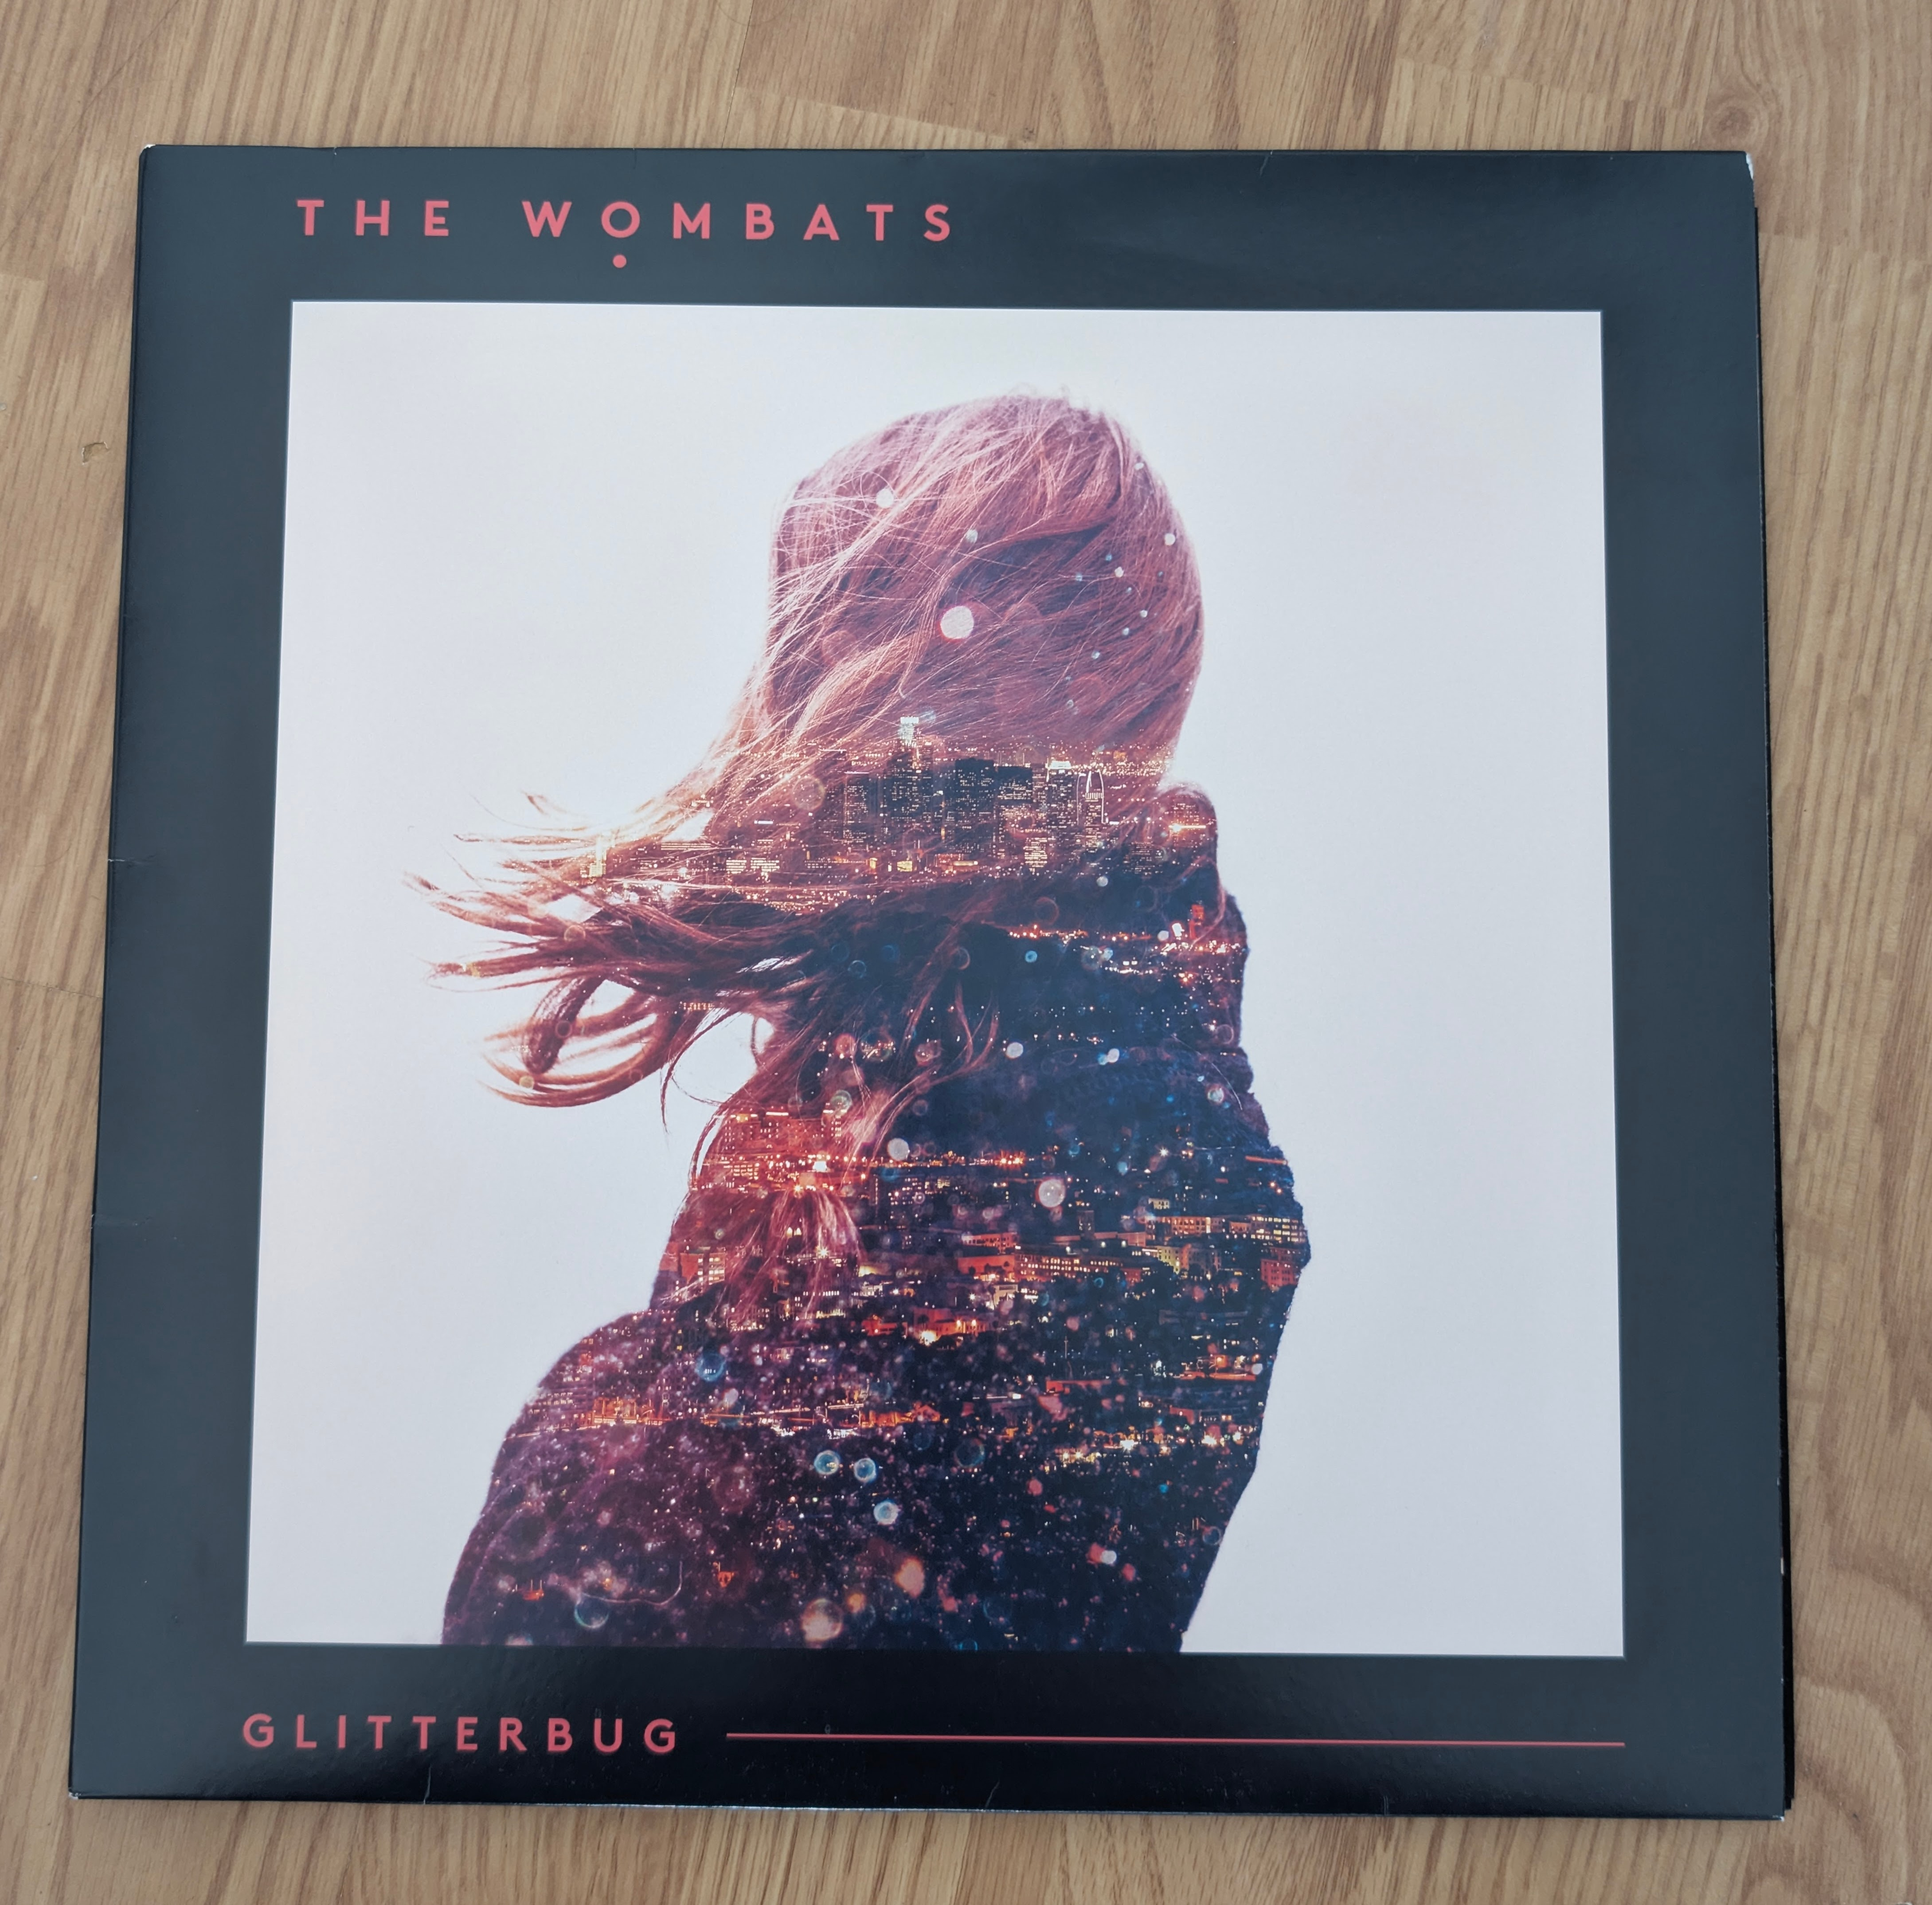
\includegraphics[width=2.5cm]{figures/test_albums/Glitterbug.jpg} \\
        \hline
        Is This What It Feels Like To Feel Like This? & The Wombats & 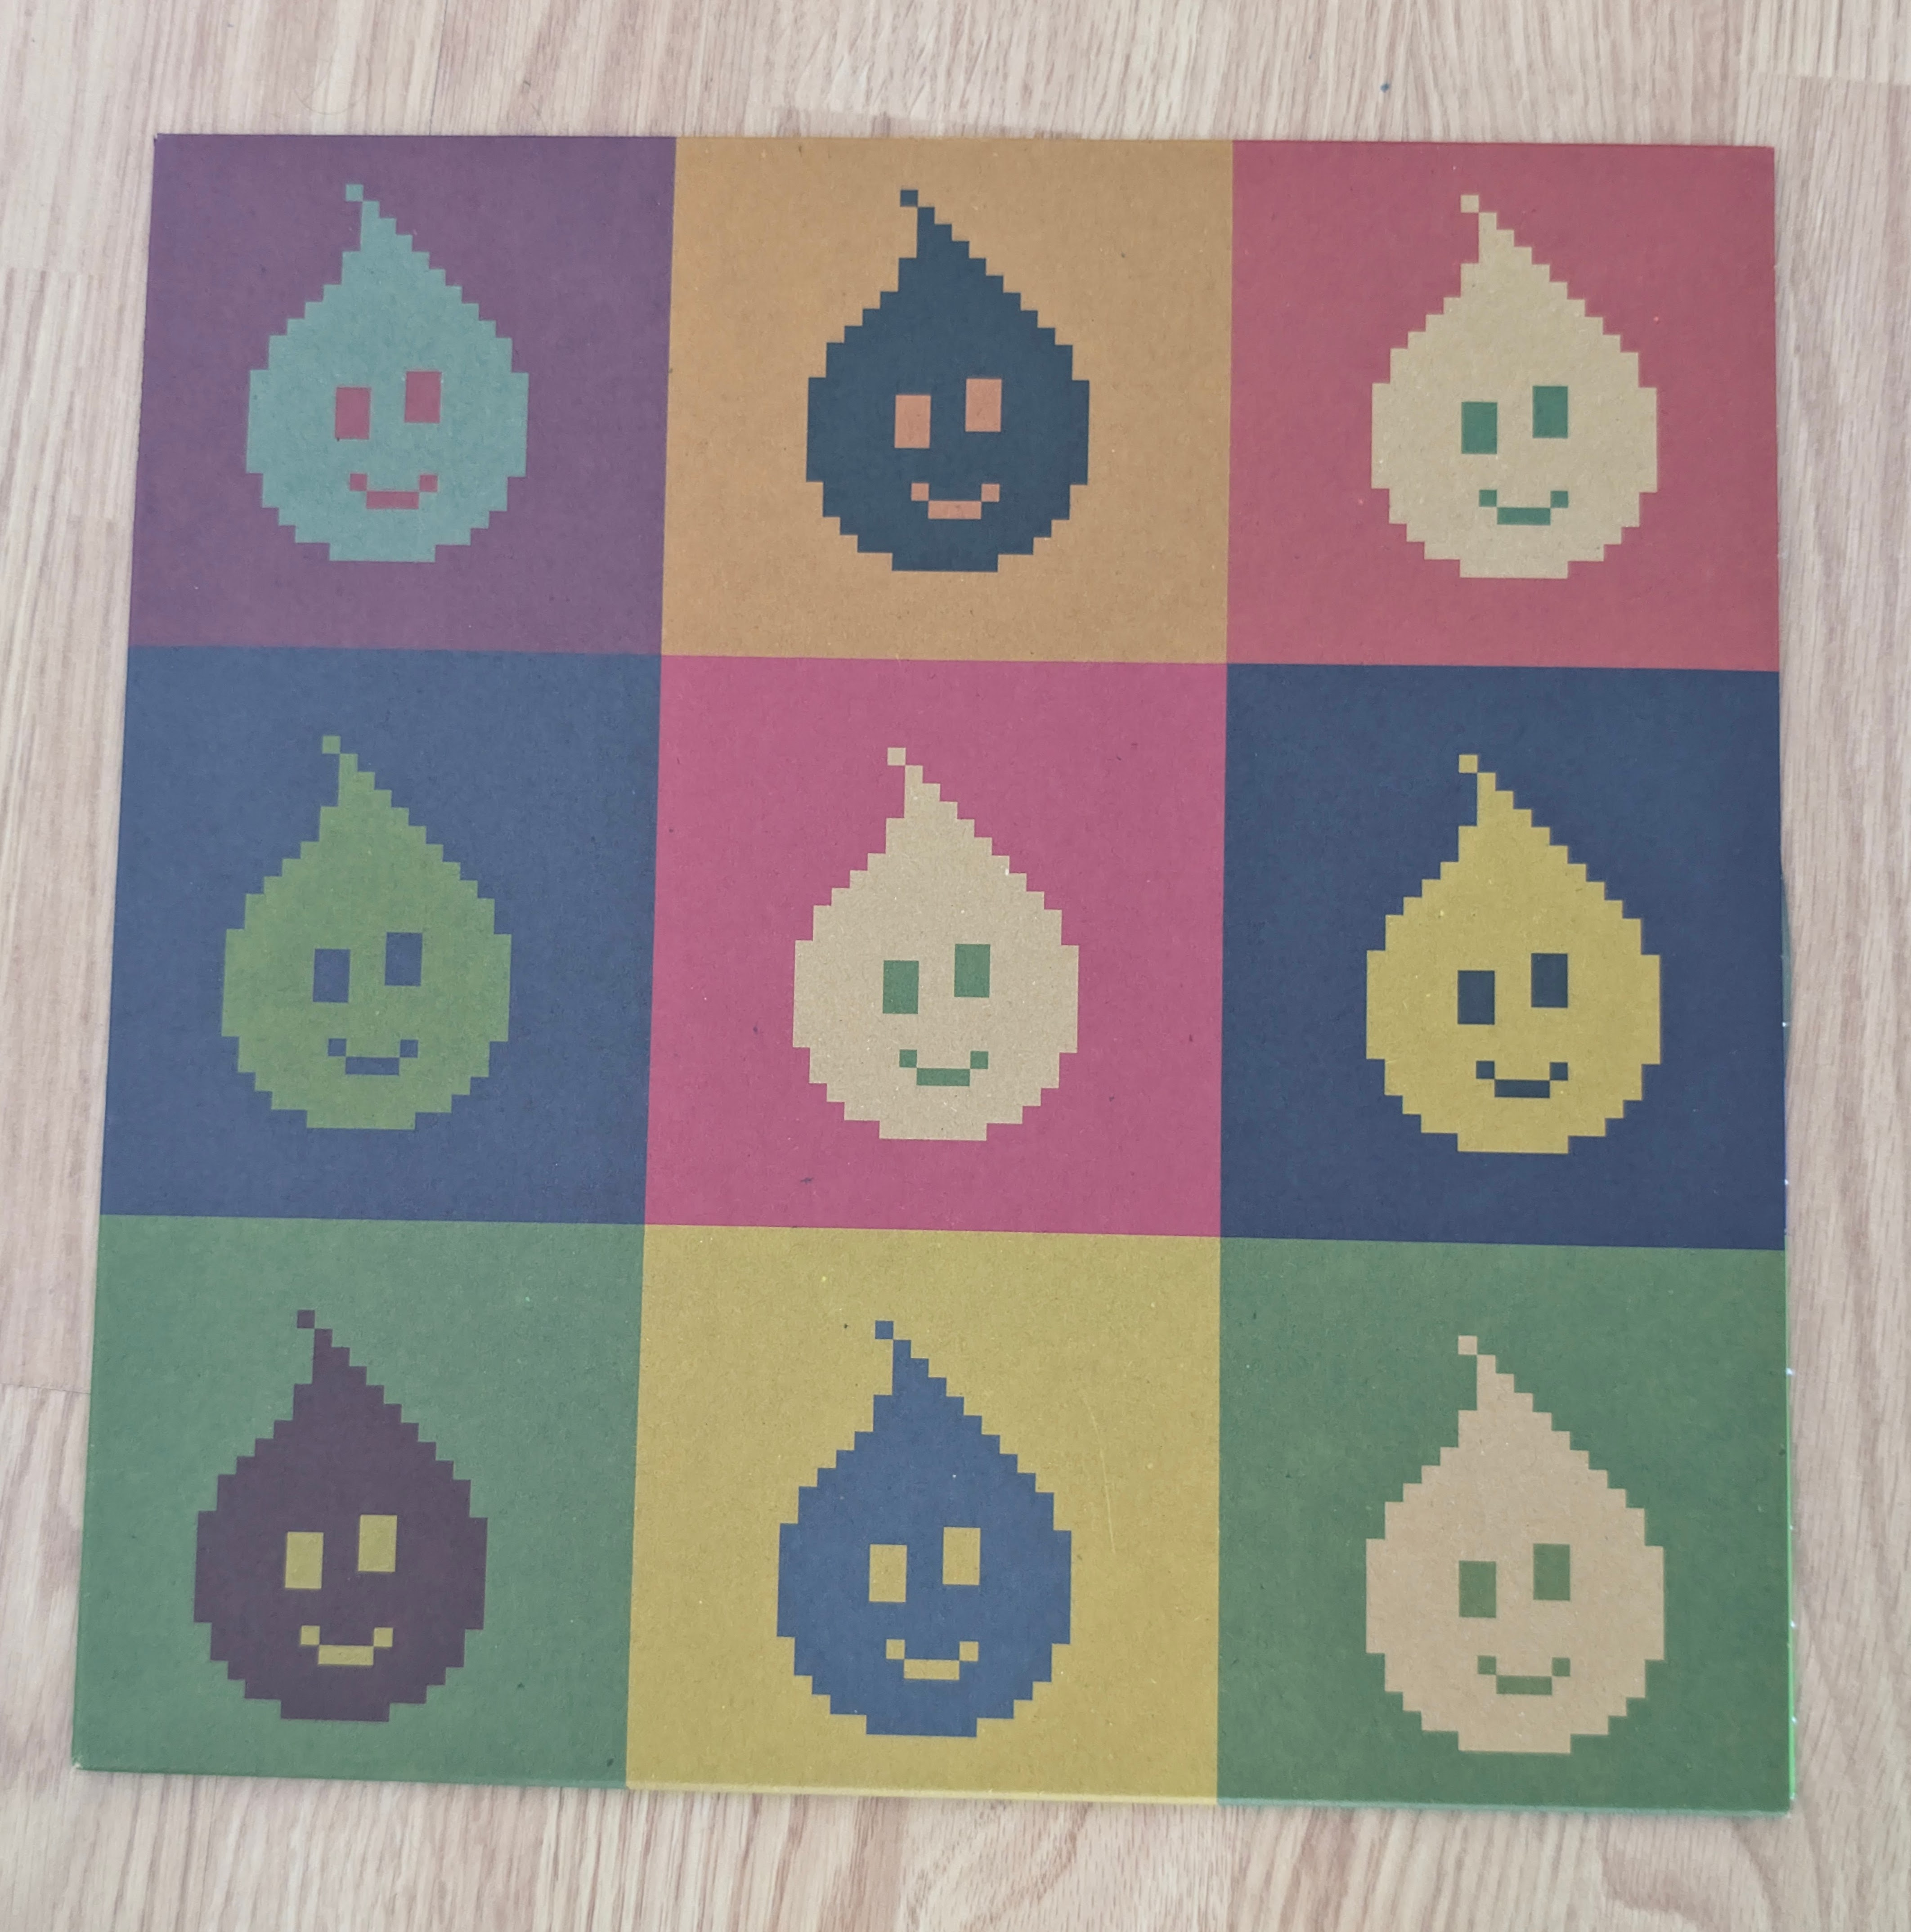
\includegraphics[width=2.5cm]{figures/test_albums/Is This What It Feels Like.jpg} \\
        \hline
        Neon Bible & Arcade Fire & 
\includegraphics[width=2.5cm]{figures/test_albums/Neon Bible.jpg} \\
        \hline
        Reflektor & Arcade Fire & 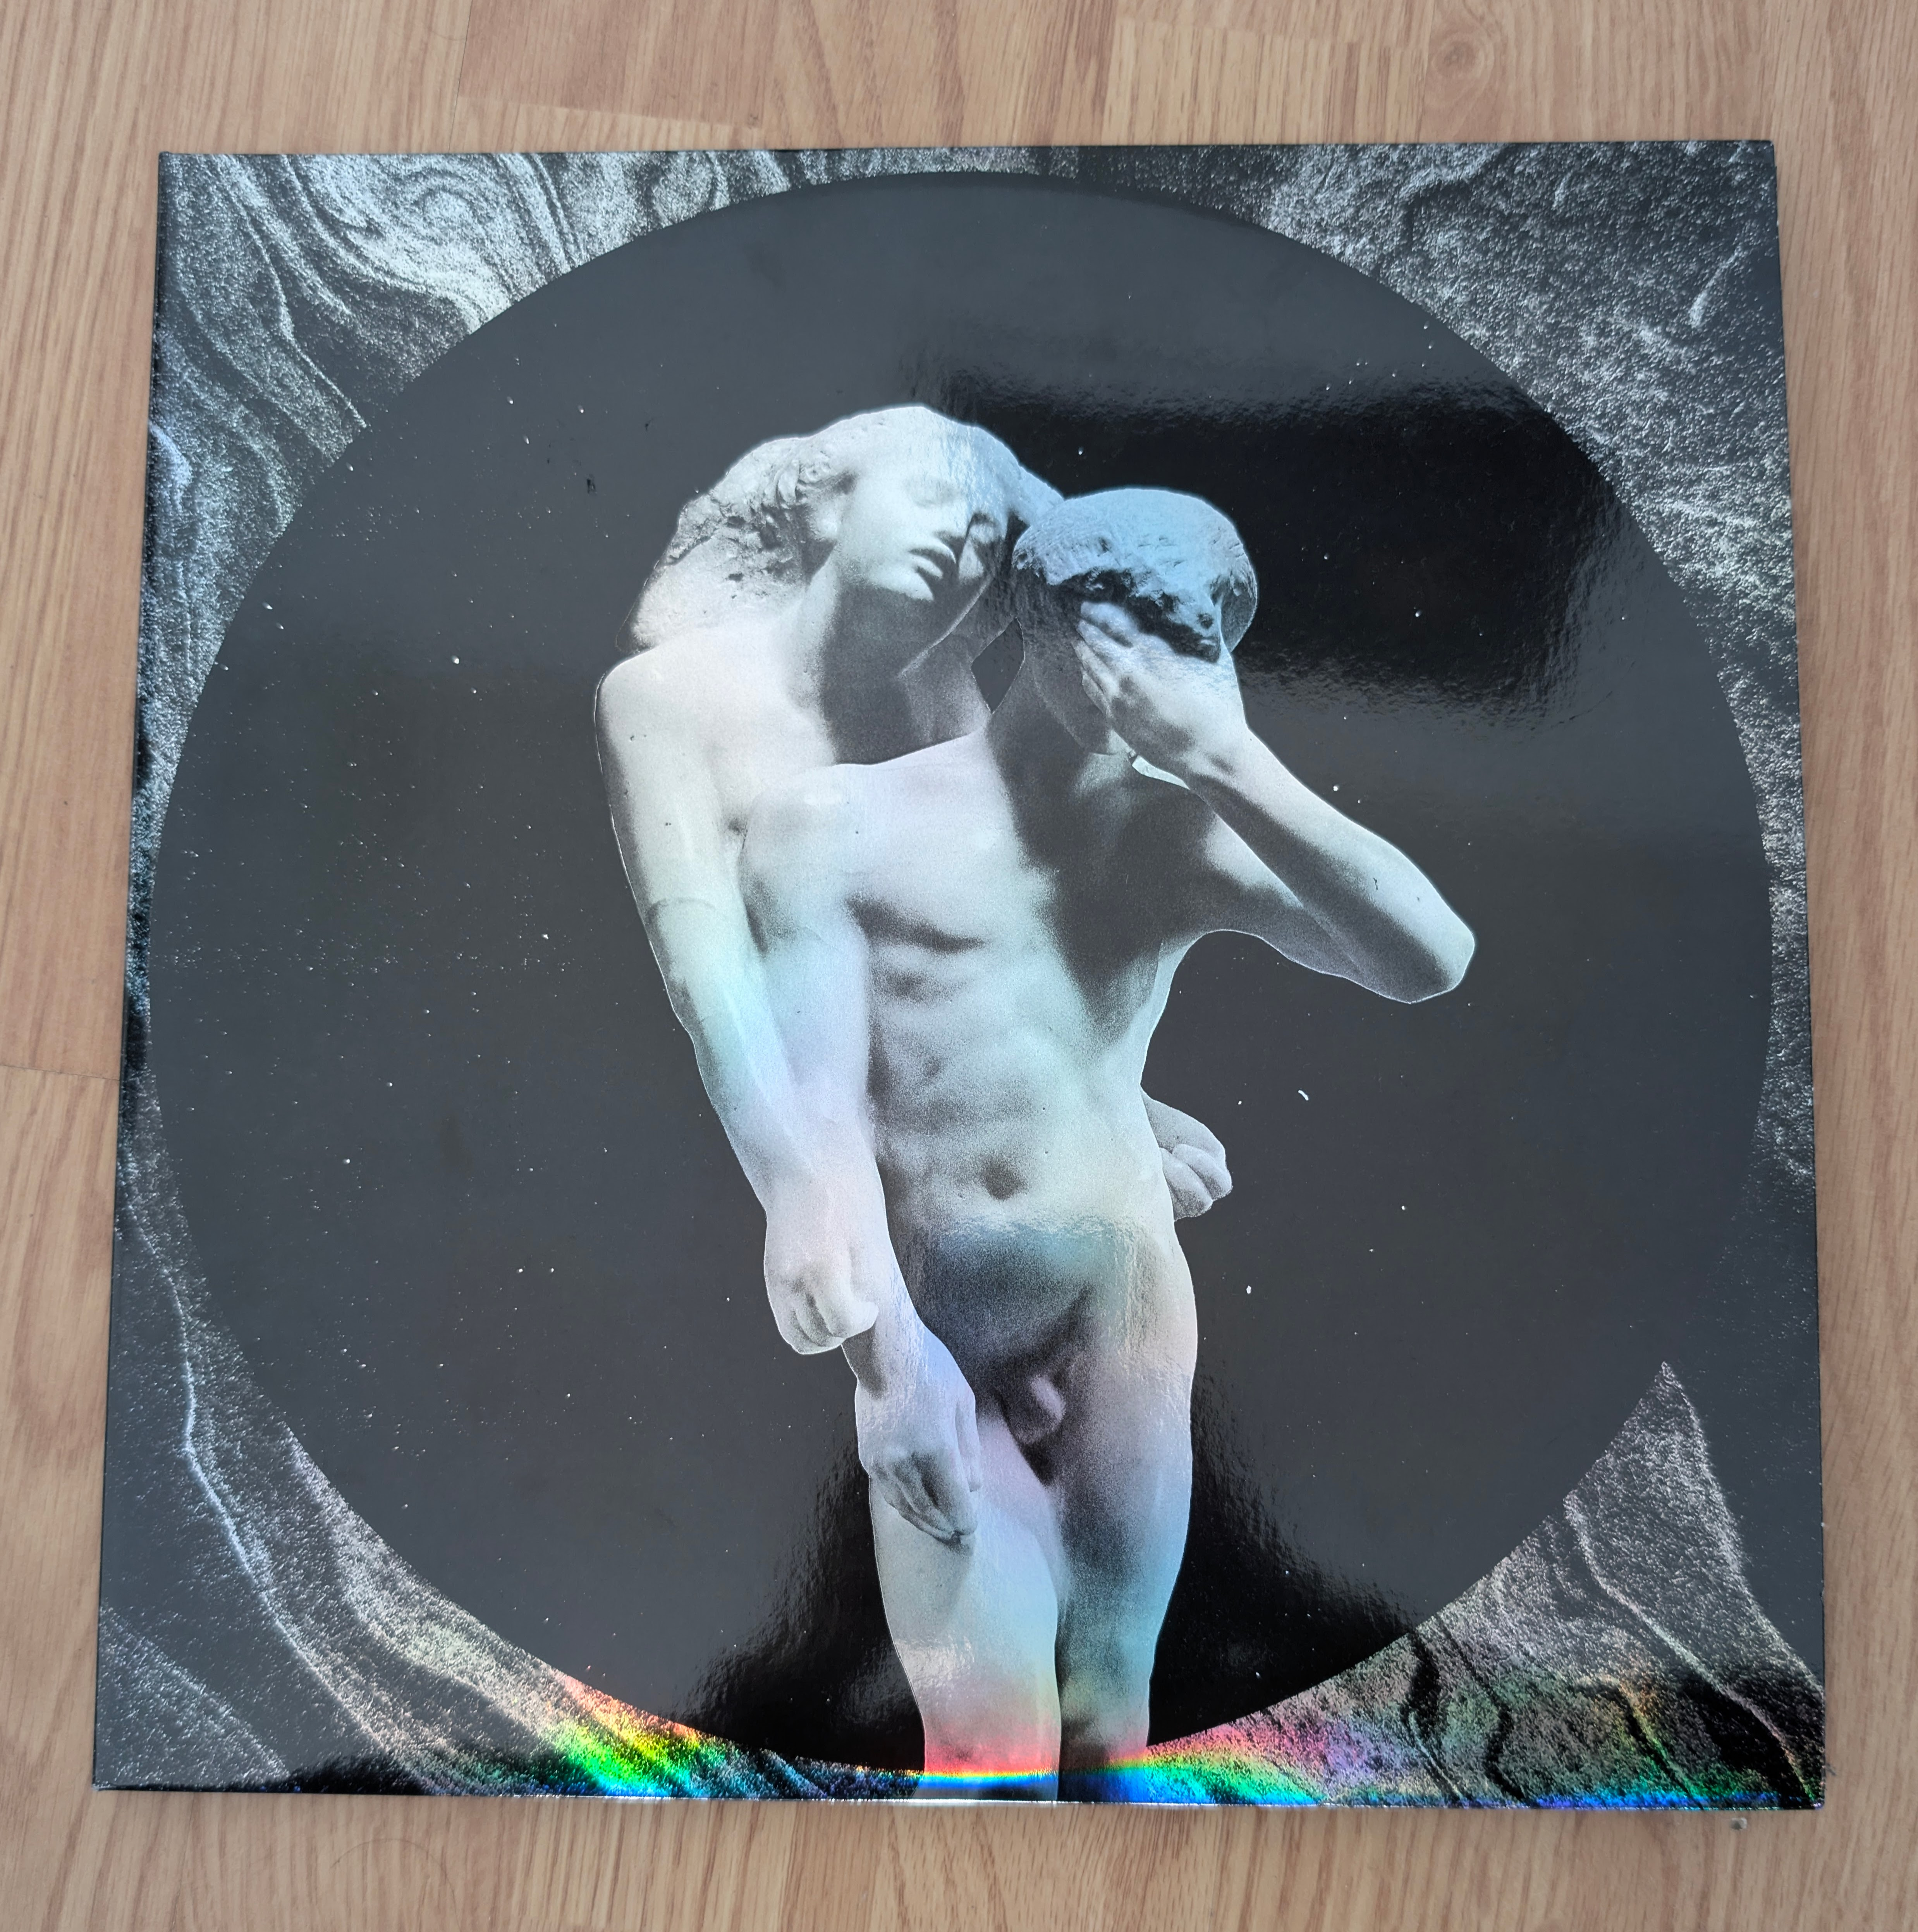
\includegraphics[width=2.5cm]{figures/test_albums/Reflektor.jpg} \\
        \hline
    \end{tabular}
    \caption{Album List continued}
    \label{tab:albums-list2}
\end{table}

\begin{table}[h]
    \centering
    \renewcommand{\arraystretch}{1.5} % Adjust row height
    \setlength{\tabcolsep}{10pt}      % Adjust column spacing
    \begin{tabular}{|m{4cm}|m{4cm}|m{4cm}|} % Adjust column widths as needed
        \hline
        \textbf{Album Name} & \textbf{Artist} & \textbf{Cover} \\
        \hline
        Sound Of Silver & LCD Soundsystem & 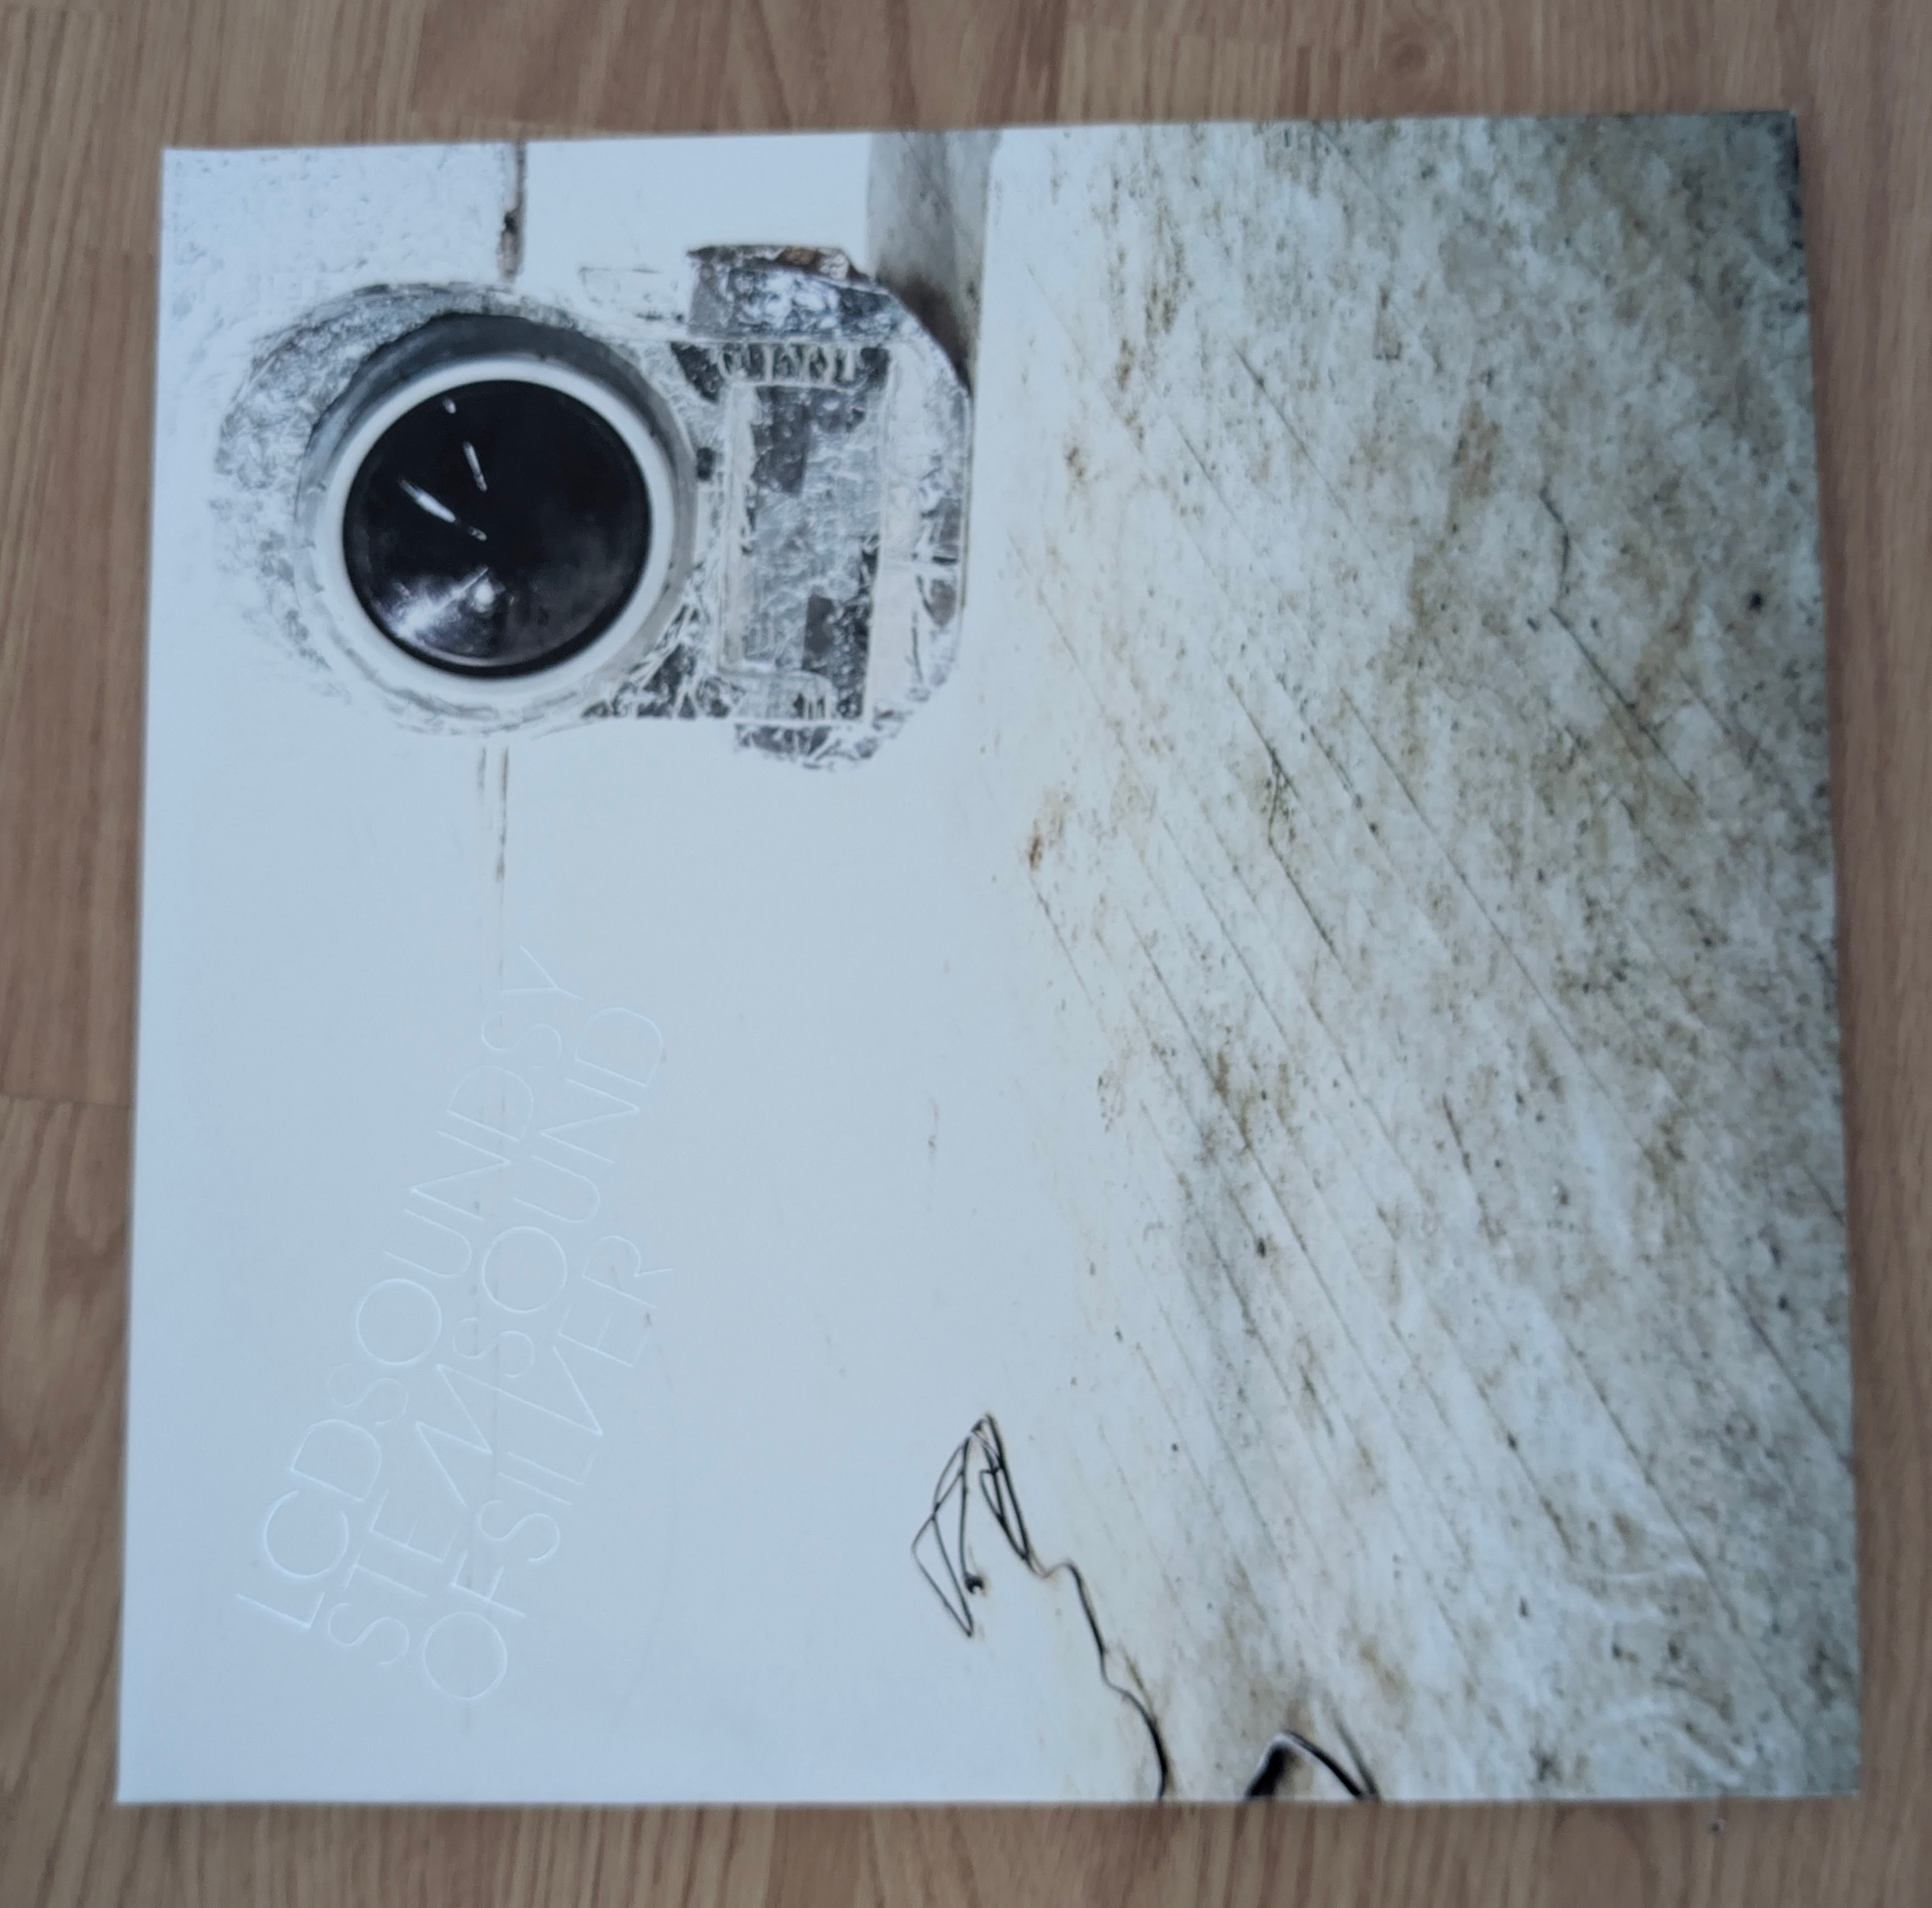
\includegraphics[width=2.5cm]{figures/test_albums/Sound Of Silver.jpg} \\
        \hline
        The Wall & Pink Floyd & 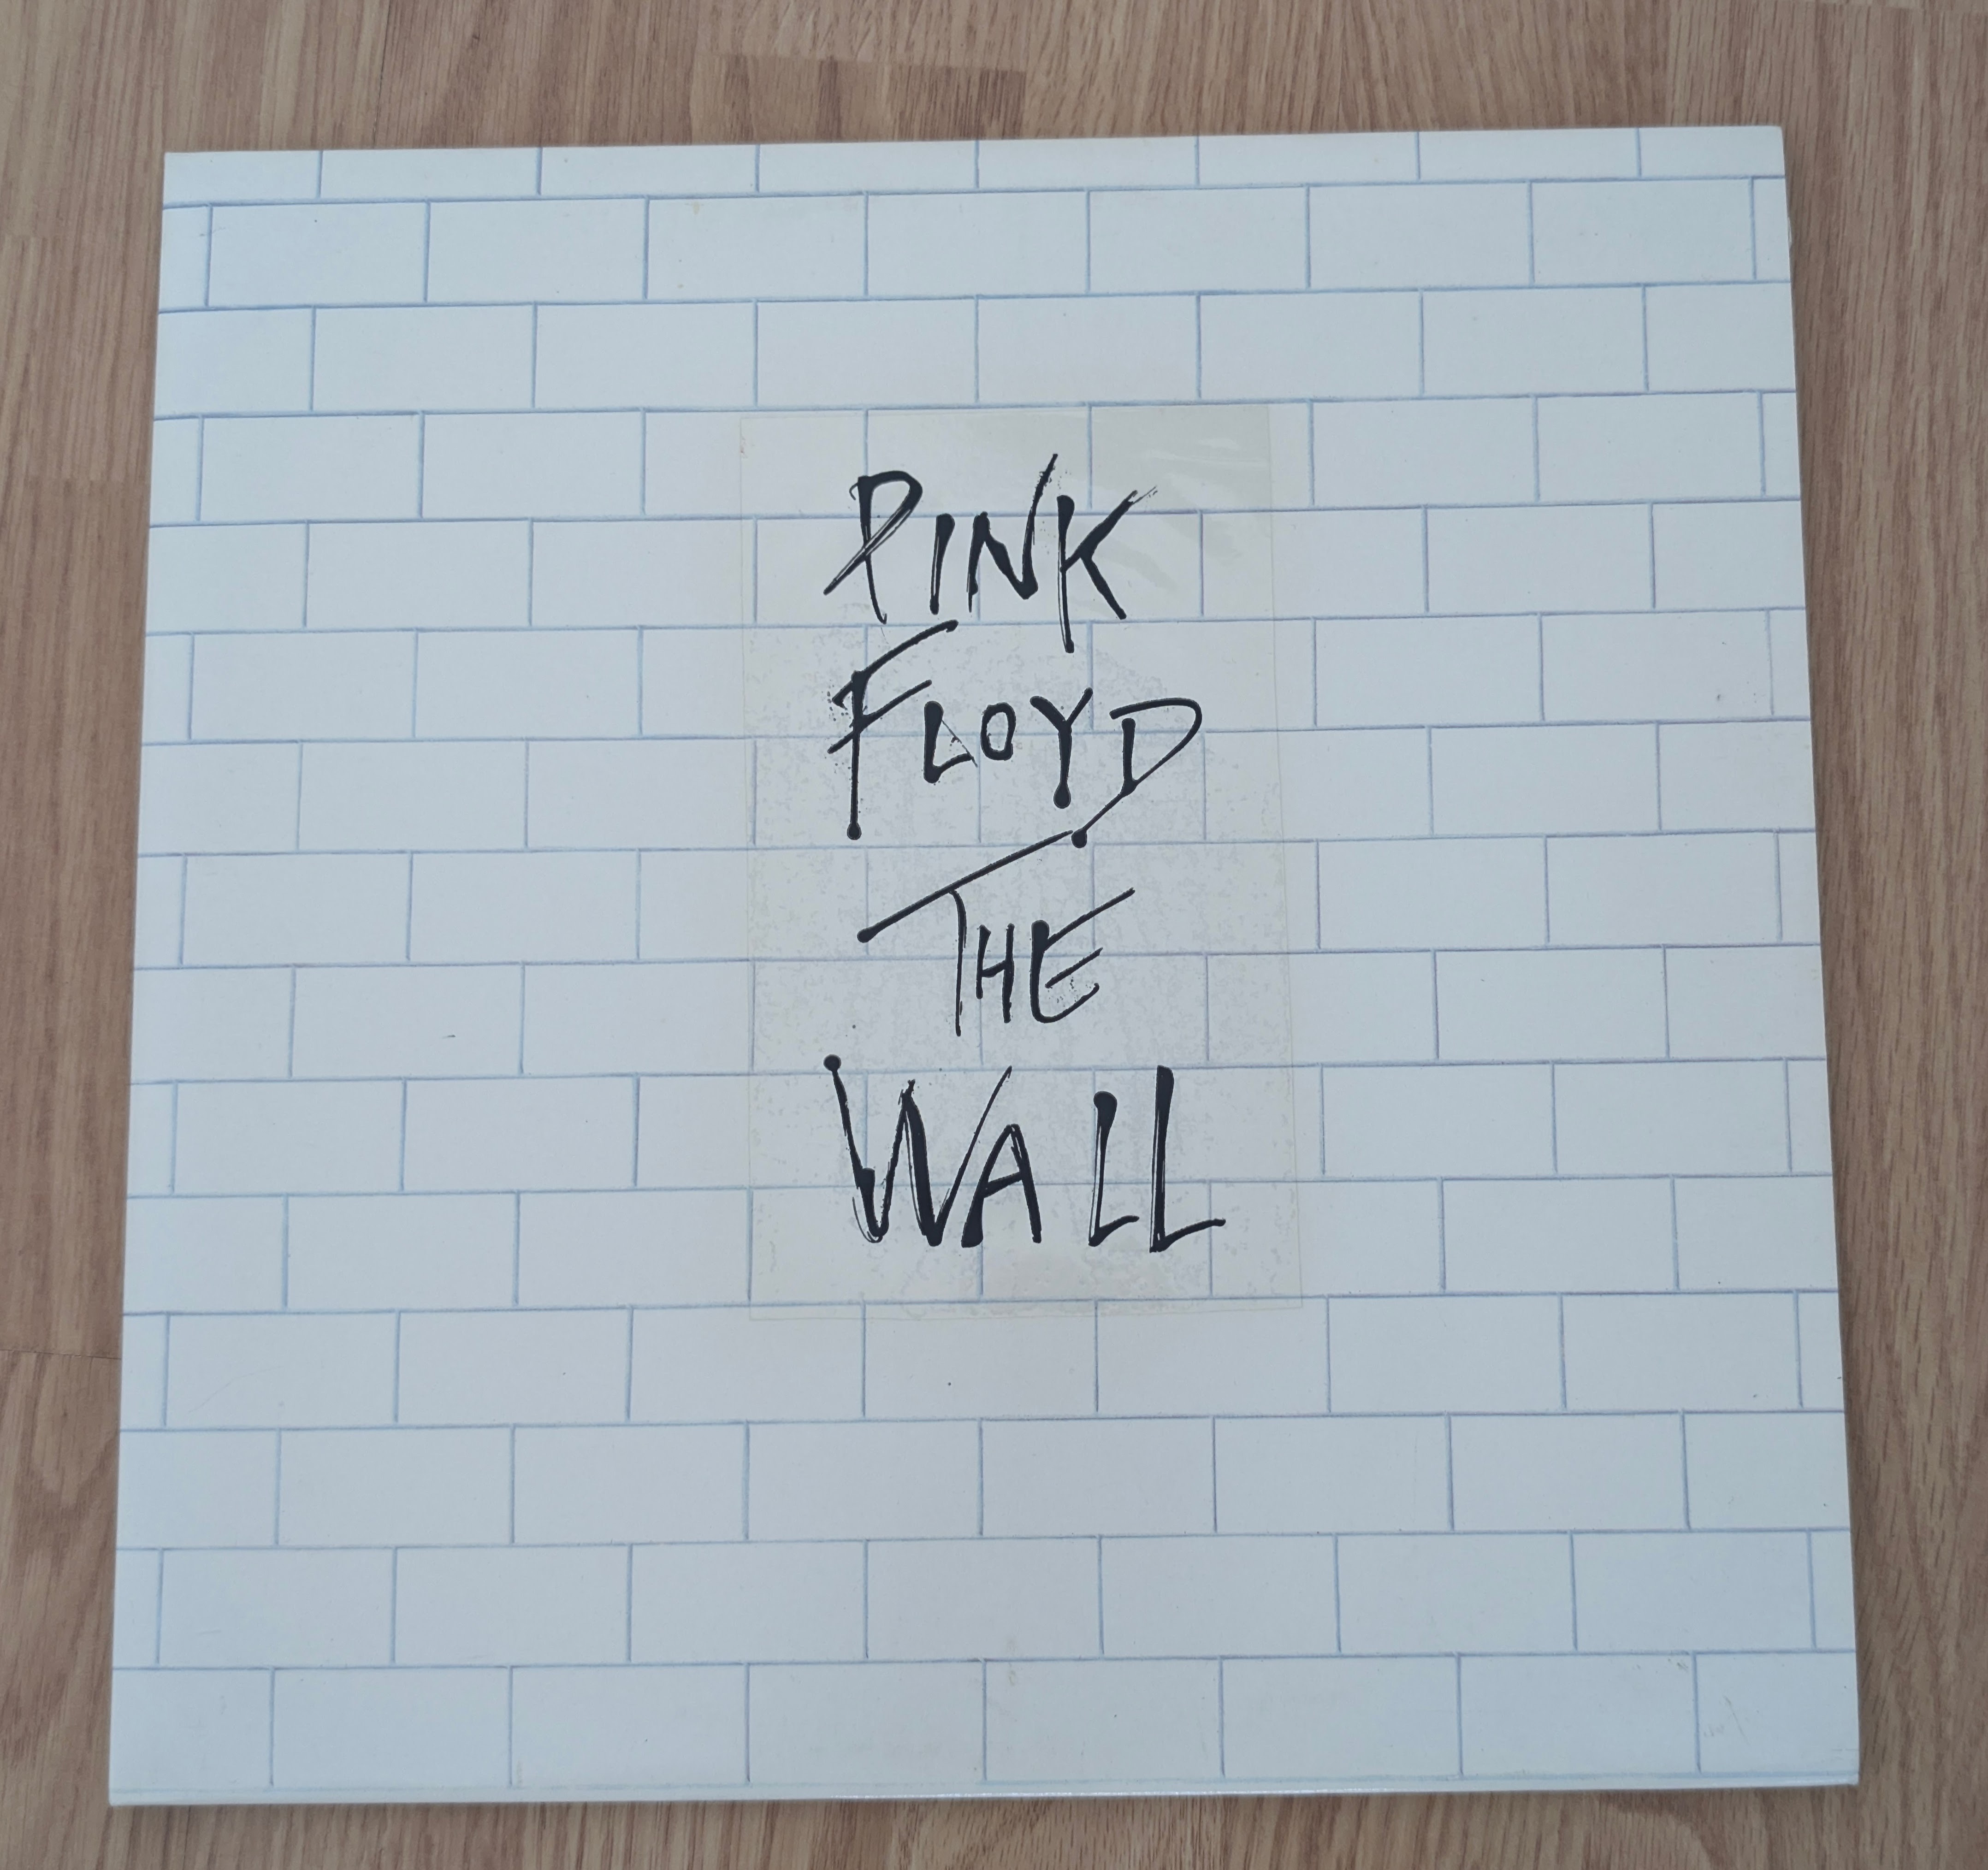
\includegraphics[width=2.5cm]{figures/test_albums/The Wall.jpg} \\
        \hline
        This is Happening & LCD Soundsystem & 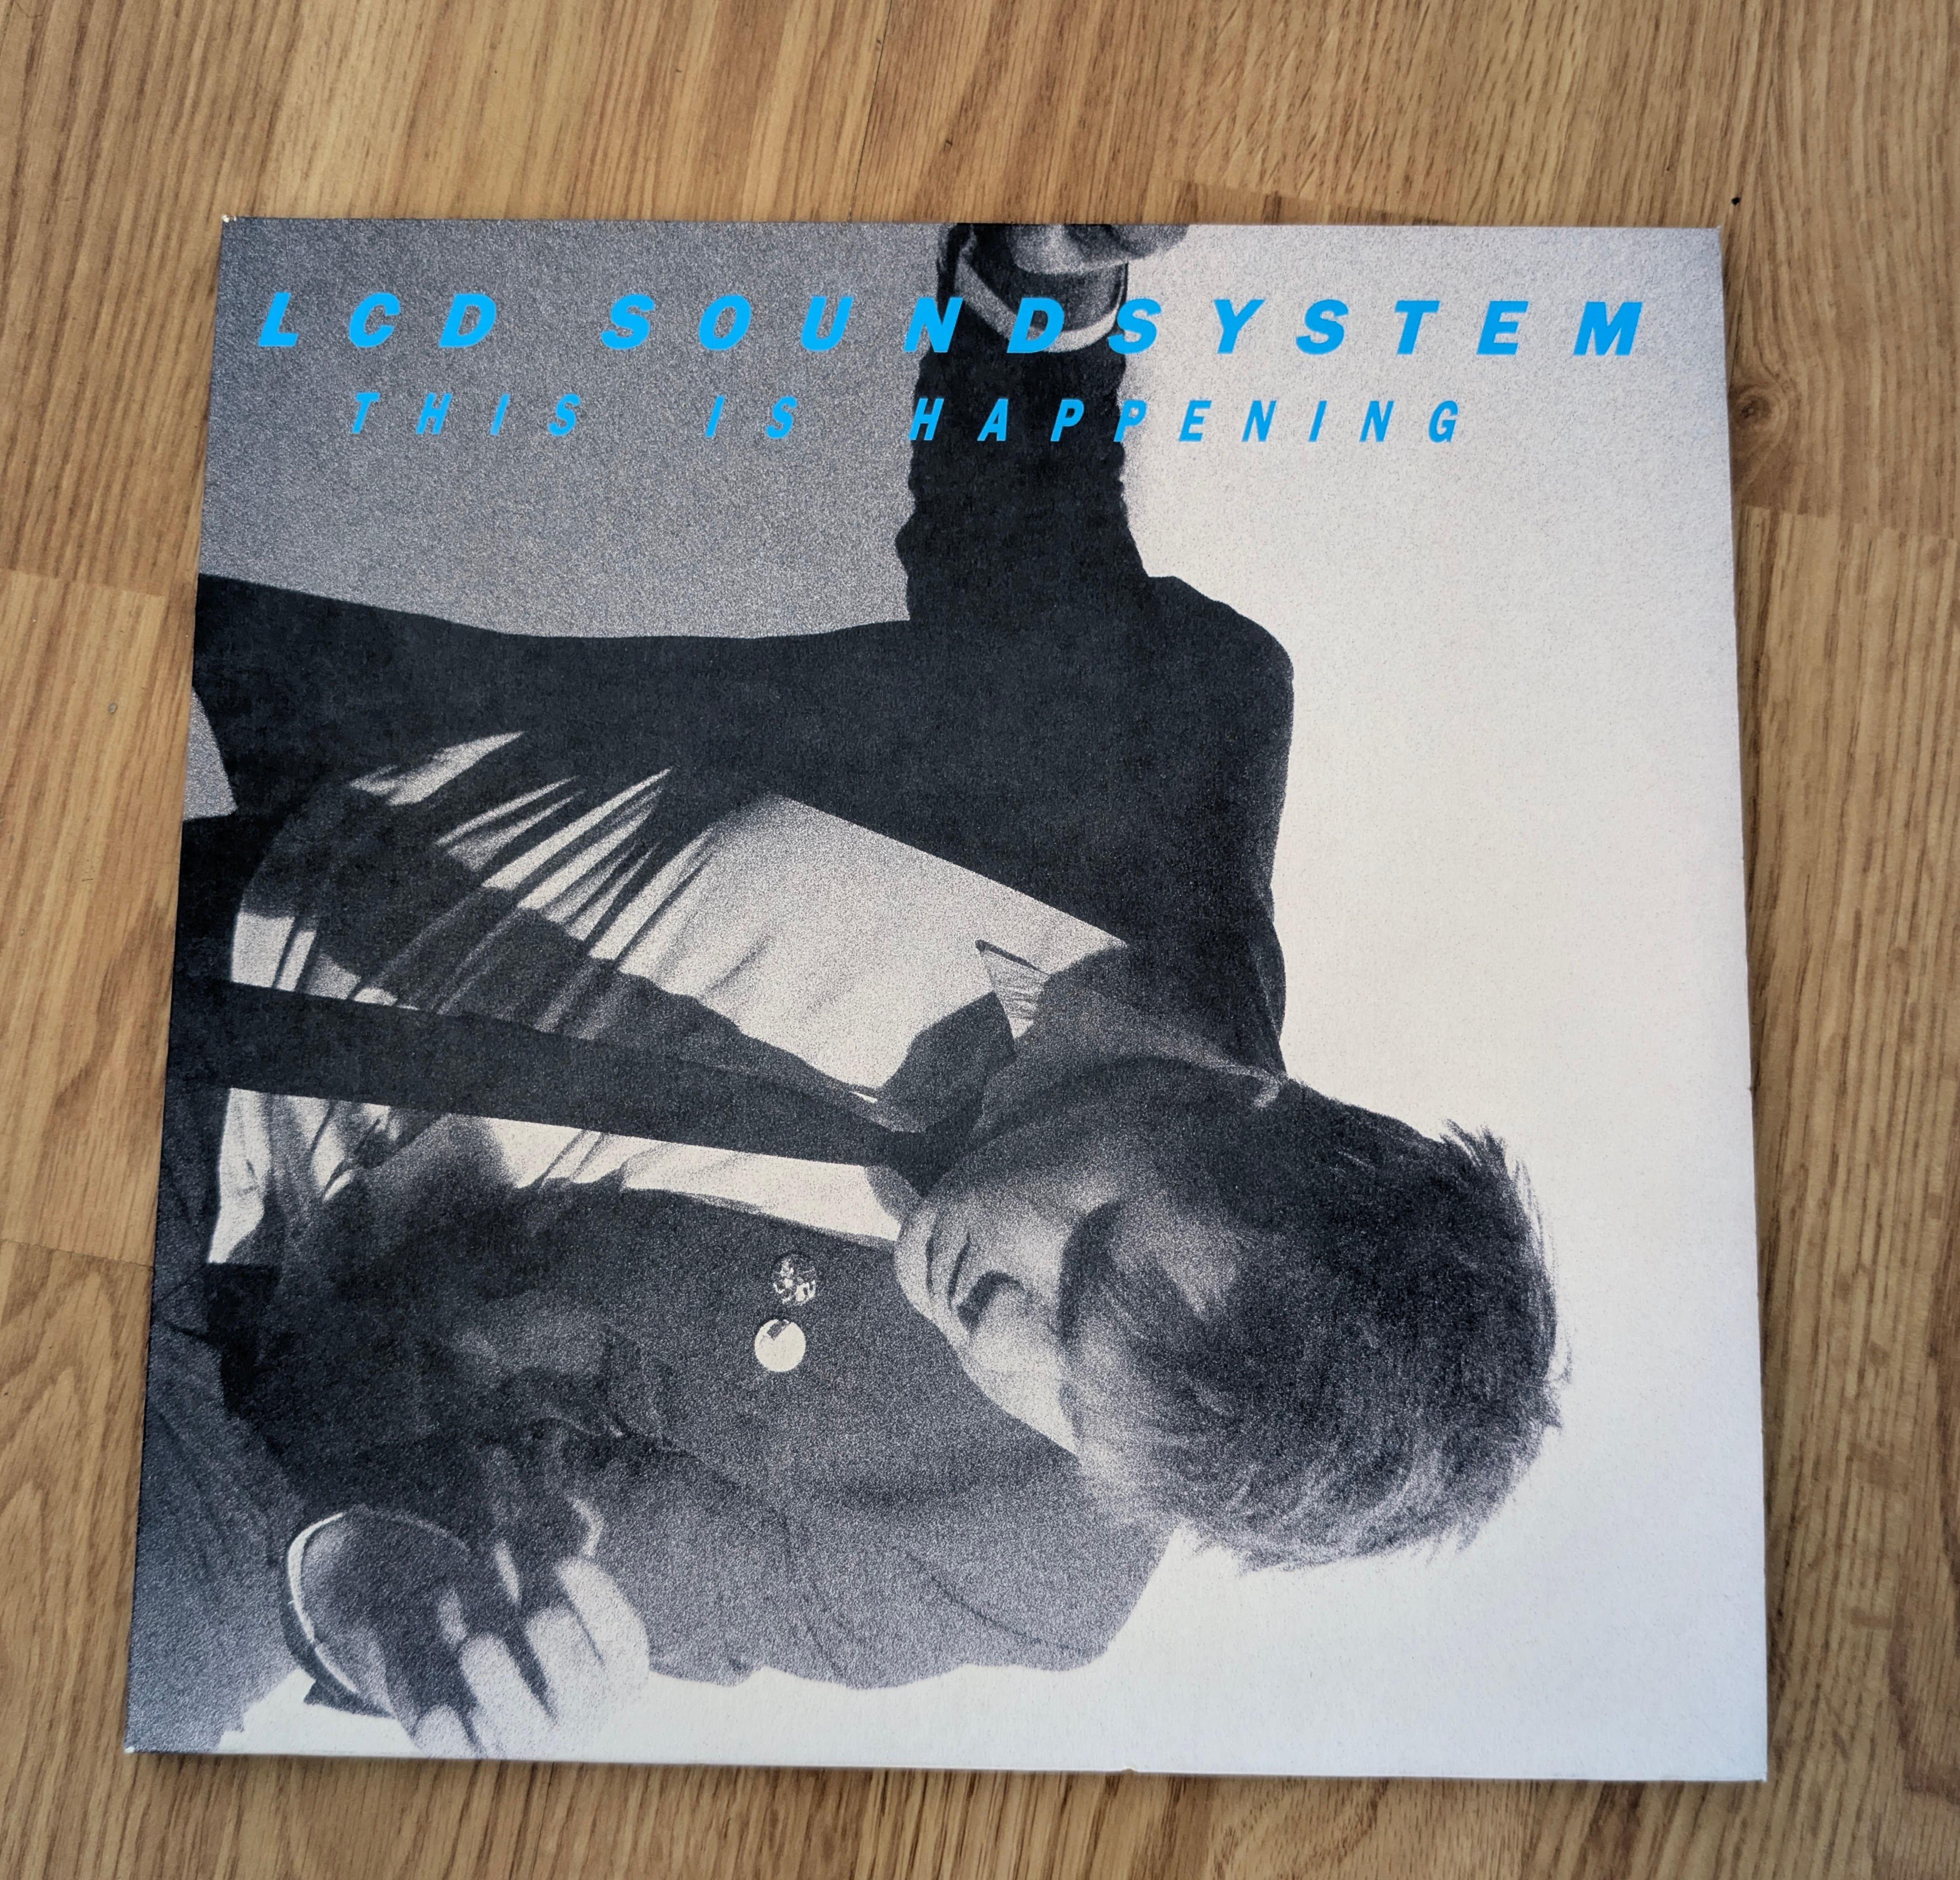
\includegraphics[width=2.5cm]{figures/test_albums/This is Happening.jpg} \\
        \hline
        We & Arcade Fire & 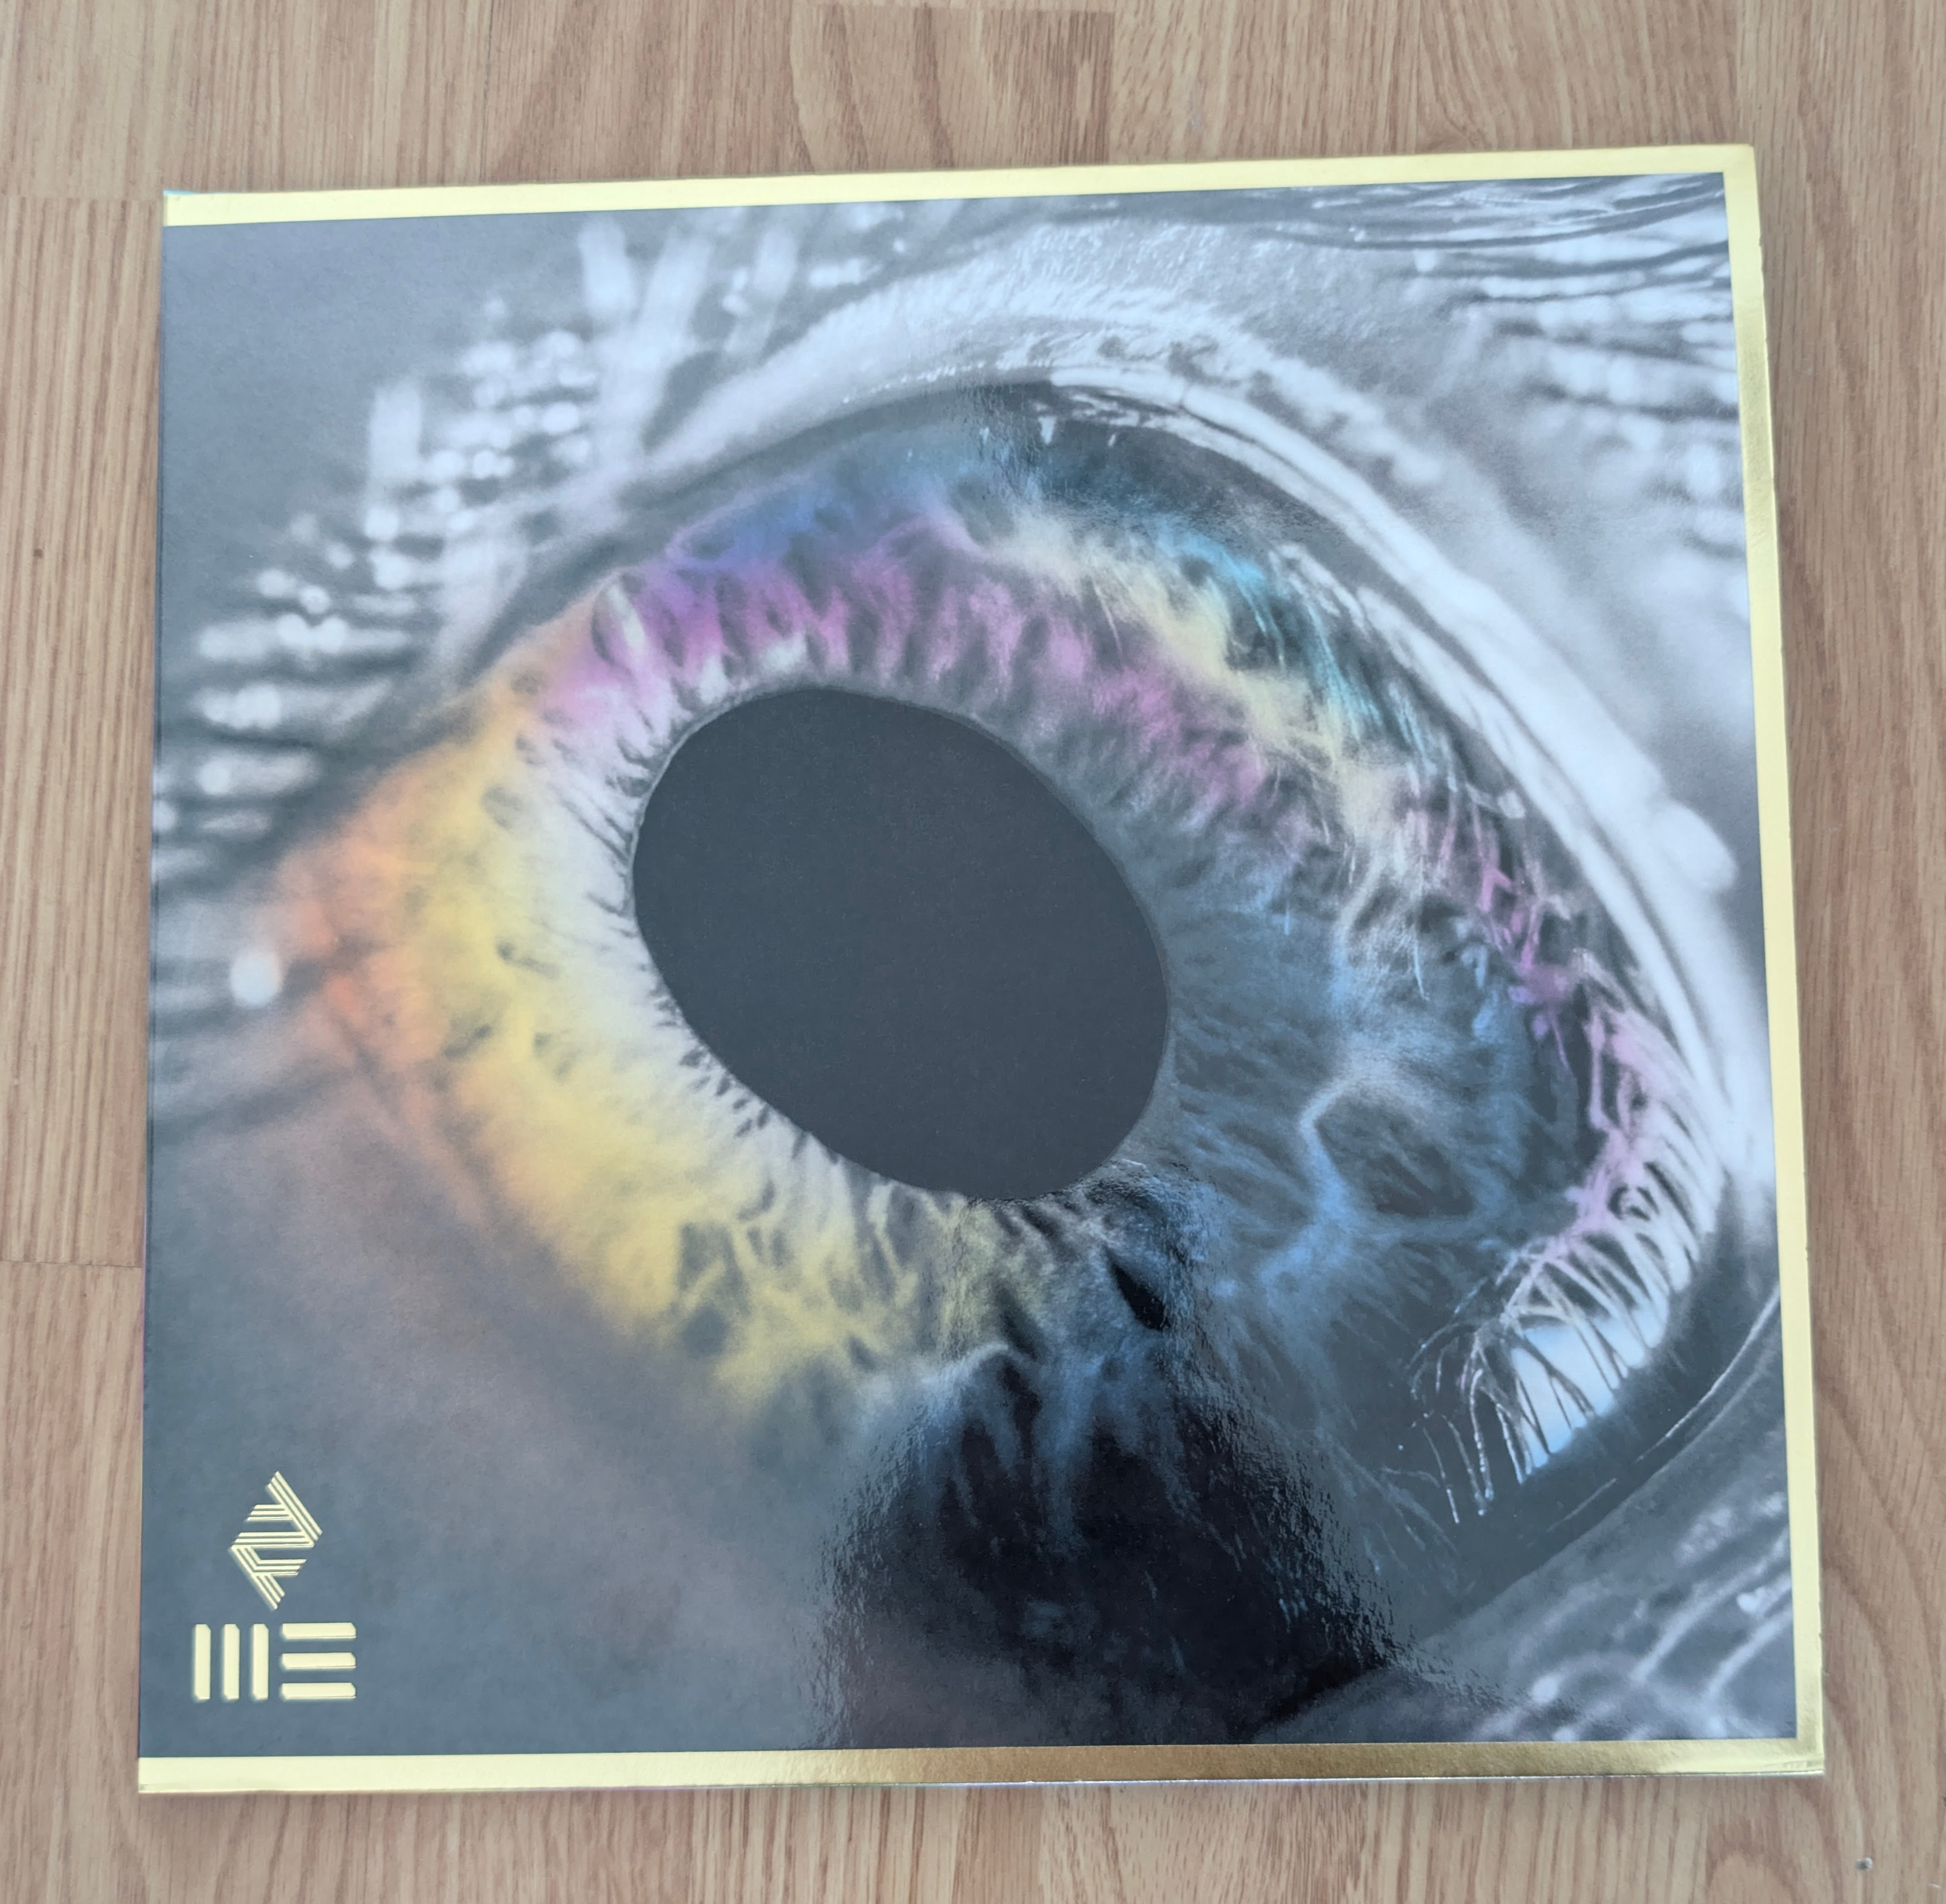
\includegraphics[width=2.5cm]{figures/test_albums/We.jpg} \\
        \hline
    \end{tabular}
    \caption{Album List continued}
    \label{tab:albums-list3}
\end{table}

\fi

\end{document}
